

\chapter{Системная биоинформатика} \label{phys_sbio}

\section{Исторический очерк математических методов в биологии}

%\begin{itemize}
%\item{Алгоритмы выравнивания}
%\end{itemize}
Коротко описывая историю развития математических методов, используемых в алгоритмах биоинформатики, как это представлено на рисунке \ref{img:methods_scheme}, следует, во-первых, отделить методы линейной алгебры и теории обыкновенных дифференциальных уравнений, которые относятся к традиционному курсу высшей математики, изучаемому в большинстве высших учебных заведений. Истоки используемых в биоинформатике методов комбинаторики, теории графов и статистики, лежат в более узких и частных, но давно разрабатываемых разделах традиционной математики. Впрочем, работы Р.Фишера (1890-1962) по классической статистике были выполнены для решения прикладных задач математической экологии, как они были поставлены в 30-х годах прошлого века, и потому применение методов статистики в вычислительной биологии имеет давнюю историю.

С именами А.А. Маркова (1856-1922), А.П. Колмогорова (1903-1987) связаны некоторые фундаментальные понятия в методах статистики и комбинаторики, используемых в биоинформатике. Но набор инструментов и подходов, обозначенный на схеме как "Функционал правдоподобия / EM (Expectation Maximization) получил свое развитие с выходом в 1977 году работы \parencite{Dempster_1977}, в которой был описан метод оценки параметров вероятностных моделей, содержащих скрытые переменные. В этой, достаточно универсальной, постановке задачи по подбору параметров математических моделей, алгоритм максимизации функционала правдоподобия оказался применим ко широкому кругу задачам биоинформатики из различных областей. Вероятностные процессы, содержащие скрытые переменные, известны как "цепи Маркова", и потому многие прикладные алгоритмы биоинформатики содержат в своей аббревиатуре или кратком описании упоминание имени А.А. Маркова.


\begin{figure}[H]
  \centering
  \vskip 12pt 
  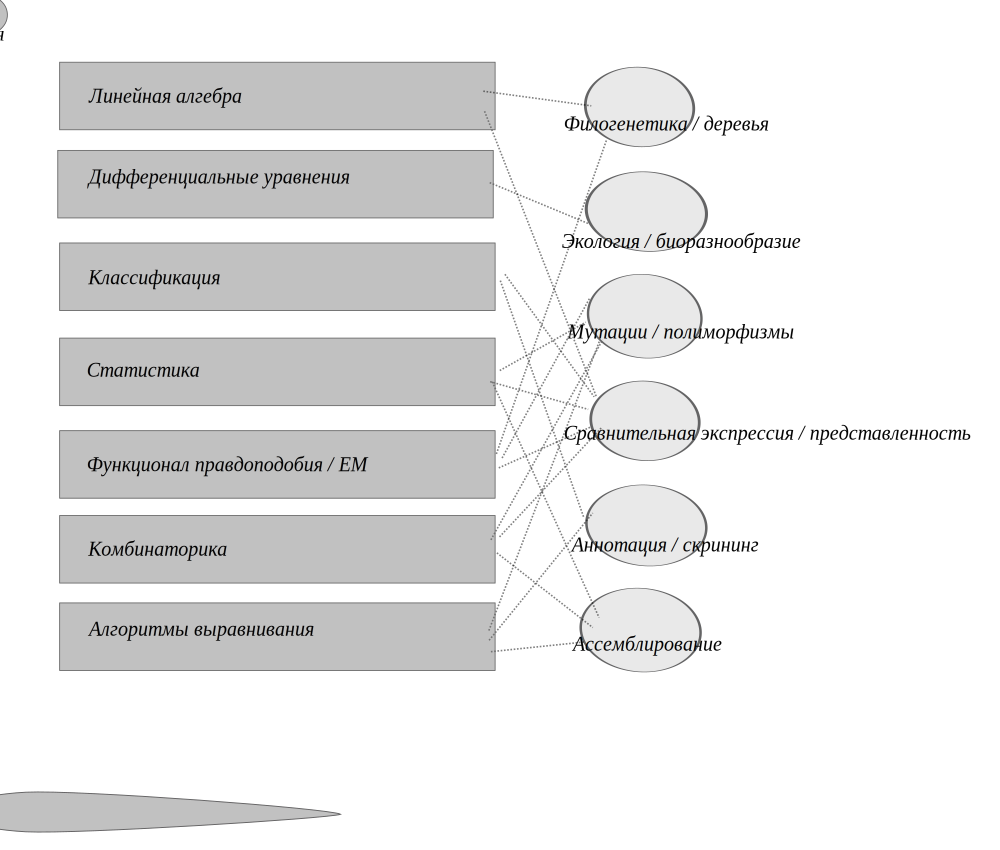
\includegraphics [width=0.8\linewidth]{methods_scheme.png}
  \vskip 12pt
  \caption[m1]{
  \textbf{Иллюстрация связи методов математики и разделов применения системной биоинформатике.}\itshape

  В правой части рисунка показаны темы системной биоинформатики, обсуждаемые в курсе, и используемые в них подходы и методы математики и информатики.
}
 \label{img:methods_scheme}
\end{figure}

Методы решения задач классификации, интенсивно разрабатываемые в современной прикладной информатике и также широко используемые в задачах биоинформатики, также можно сгруппировать на основании подходов, лежащих в их основе. Подходов к решению задач классификации относительно немного; наиболее популярным в последние десятилетия является подход на основе метода опорных векторов, разрабатываемого с 1963 г. В. Вапником с соавторами (см. \parencite{Вапник_1974}).  

Алгоритмы выравнивания биологических последовательностей, отдельно помеченные на схеме \ref{img:methods_scheme}, лежат в основе значительной части прикладных методов биоинформатики. В развитии этих алгоритмов следует упомянуть несколько ключевых идей, появление каждой из которых способствовало значительному прогрессу при решении прикладных задач. Это, во-первых, алгоритм поиска оптимального выравнивания двух последовательностей аминокислот \parencite{Needleman_1970}, реализуемый в рамках алгоритмической теории называемой \textit{динамическим программированием}. Также, использование преобразования Барроуза — Уилера \parencite{Burrows_1994} сделало возможным быстрый и эффективный поиск гомологичных фрагментов в базах последовательностей ДНК, на основании попарного выравнивания с последовательностью-шаблоном.

Среди алгоритмов и идей, оказавшихся важными для прогресса в других разделах биоинформатики, следует также упомянуть алгоритм ассемблирования фрагментов ДНК \parencite{Idury_1995} с использованием понятия \textit{графа де Бройна}, а также алгоритмы для построения филогенетических деревьев, развитие которых началось в конце 1960х \parencite{Fitch_1967,Felsenstein_1981}. Но впрочем, задачи построения филогенетических деревьев, множественного выравнивания последовательностей, быстрого поиска гомологов в базах данных неизбежно требуют введения эмпирических приближений для ускорения времени расчетов, и потому результаты расчетов в таких задачах не всегда являются оптимальными по формальным критериям.  

\begin{figure}[H]
  \centering
  \vskip 12pt 
  \includegraphics [width=0.95\linewidth]{matematicians.png}
  \vskip 12pt
  \caption[m1]{
  \textbf{Некоторые из ученых, работы которых лежат в основании подходов в системной биоинформатике}\itshape

  А.А. Марков (1856-1922), Р. Фишер (1890-1962), Н.В. Тимофеев-Ресовский (1900-1981), А.П. Колмогоров (1903-1987), К. Шеннон (1916-2001), Б. Мандельброт (1924-2010).
} 
 \label{img:matematicians}
\end{figure}

Использование дифференциальных уравнений для описания характерных свойств в поведении экосистем, начатое в 1920х годах (модель "хищник-жертва") и развитое в России в научной школе, основанной Н.В. Тимофеевым-Ресовским, обычно не подразумевает возможности детализации моделей экосистем до молекулярного уровня. Но при неизбежности введения эмпирических упрощений в расчеты основанные на молекулярном представлении сложных биологических объектов, следует подчеркнуть значимость результатов, полученных при таком подходе. И, наконец, в обзоре подходов для анализа биологических систем следует упомянуть теорию фракталов; понятия фрактала и фрактальной размерности, введенные в работах Б.Мандельброта 1960х-1970х годов, являются еще в большей степени универсальным методом описания сложных систем, без возможности проследить связь наблюдаемых эффектов с молекулярным представлением объектов.


%Количественный анализ биологических моделей основывается на использовании законов физики, химии, математического аппарата теории дифференциальных уравнений и статистики. Методы биоинформатики позволяют уточнять свойства объектов биологических систем и связей между ними, таких как химическое сродство между белками, регуляция экспрессии определенного гена, эволюционная близость организмов.

%Формальная сторона такого рода систем подразумевает использование математического аппарата теории графов. Теория графов может быть построена, если задано произвольное множество вершин V и множество ребер как подмножество множества пар вершин V*V. В ряде систем полезным является математическое представление теории категорий, когда задан класс объектов V и для каждой пары объектов задано множество морфизмов V○V с определенными свойствами.

%Математические модели сетей в биологии используют для того,  чтобы описать поведение модельной системы. В некоторых случаях произвести предсказания, которые можно сравнить с экспериментальными наблюдениями. Методы моделирования таких сетей включают использование систем обыкновенных дифференциальных уравнений, а также булевские сети, сети Петри, байесовы сети, стохастические сети и др.


%Системы дифференциальных уравнений в математической биологии могут иметь очень различающиеся особенности и структуру в зависимости от конкретной задачи. Так, при моделировании сетей метаболизма или регуляции генов при помощи обыкновенных дифференциальных уравнений. Такие уравнения в общем случае записываются как dSi/dt=fi(S1..SN), где N — количество элементов в системе, S1,S2,..SN –  концентрации соответствующих веществ. Конкретная форма зависимостей fi  выводится на основе законов химической кинетики и часто представляет из себя полином. Анализируя такие уравнения, можно найти устойчивые состояния системы, где dSi/dt = 0.

%Устойчивые состояния кинетических уравнений, таким образом, соответствуют потенциальным типам клетки, а колебательные решения уравнений — типам клетки которым присущи естественные циклические колебания. Критические точки и раздвоения в уравнениях соответствуют критическим состояниям клетки, в которых небольшое возмущения параметра может переключить систему между одной из нескольких стабильных ветвей дифференцирования. Траектории соответствуют разворачиванию биологических путей, а переходные процессы уравнений - краткосрочным биологическим событиям.


\section{Иерархия объектов в системной биоинформатике} \label{sect1_1}

%Биоинформатика является инструментом биологии и методы биоинформатики применяют при анализе различных биологических систем. Также биоинформатика, как совокупность прикладных компьютерных методов, может быть рассмотрена как информационная система в широком смысле. Информационная система характеризуется данными, программами для их обработки и аппаратным обеспечением. Данные, с которыми оперирует биоинформатика, соответствуют объектам биологических систем.

%Методы биоинформатики, которые позволяют уточнить свойства сетей регуляции генов, включают анализ корреляций в экспериментах по измерению уровня экспрессии генов определяемой по уровню матричной  РНК  гена в клетке, а также анализ экспериментов с использованим метода масс-спектрометрии, которые позволяют определить белки содержащиеся в исследуемом образце. 

%Важное значение для получения информации о взаимодействии белков и генов также имеет автоматический анализ научных текстов. Наконец, информацию о взаимодействии белков с другими белками и прочими молекулами можно получить из моделирования пространственного взаимодействия этих молекул. Также информация о гомологии белков и РНК между различными организмами и внутри одного организма позволяет расширить и обобщить информацию о взаимодействии белков. 

%В биоинформатике  как и в биологии в целом происходит интенсивное накопление знаний о биологических системах. Эти знания также требуют систематизации.  В информационных технологиях и компьютерных науках часто используется представление таких знаний как явная спецификация описаний множества объектов и связей между ними, называемая онтологией.

%Бурное развитие молекулярной биологии и генетики в конце 20-ого – начале 21-ого веков привело к накоплению огромного массива экспериментальных данных, в первую очередь последовательностей ДНК, РНК и белков, цифровых биологических изображений и структур сигнальных сетей, хранение и анализ которых не возможен без применения соответствующего ПО. Хотя и раньше информационные технологии использовались биологами, например, для статистической обработки полученных данных, именно бум молекулярной биологии вызвал у специалистов-биологов потребность в специализированных инструментах для решения конкретных задач по обработке биологической информации. С этим связано возникновение БИ как самостоятельной области науки. Уже сейчас большинство исследователей в области молекулярной биологии и генетики пользуются биоинформационными инструментами на этапе планирования эксперимента и обработки полученных экспериментальных данных. Более того, имеется большое количество опубликованных работ, полностью основанных на применении БИ для решения конкретных биологических проблем. Вполне вероятно, что в перспективе будет возможным компьютерное моделирование биологических систем различной сложности, что позволит вывести биологию на принципиально иной уровень.

При перечислении дисциплин и предметных областей биологии, где используются подходы, которые можно объединить словом "биоинформатика", следует использовать, во-первых, масштабы и уровень детализации изучаемых объектов. Но также, развитие многих прикладных методов и пакетов программ в биоинформатике связано с развитием экспериментальных методов и методик постановки экспериментов. В частности, бурное развитие вычислительных методов, используемых для обработки больших объемов нуклеотидных последовательностей, можно связать с появлением в 2000-2010 гг. так называемых технологий \textit{секвенирования нового поколения} (\textit{высокопроизводительного секвенирования}), позволяющих эффективно "считывать" информацию, содержащуюся в ДНК. 

При появлении этих технологий, развитие получили, в первую очередь, методы изучения живой клетки и систем регуляции в клетке на молекулярном уровне (таблица \ref{tab:methods_hier}). Дополнительными экспериментальными методами при изучении живой клетки стали масс-спектрометрия и технология, использующая гибридизацию фрагментов ДНК в так называемых \textit{микрочипах}. Методы обработки экспериментов по масс-спектрометрии развились в дисциплины, называемые \textit{метаболомикой} и \textit{протеомикой}. 


\renewcommand\theadalign{bc}
\renewcommand\theadfont{\fontsize{14pt}{16pt}\selectfont}

\begin{table}[htbp]
\caption{Уровни детализации в задачах биоинформатики}\label{tab:methods_hier}
\begin{tabular}{|l|l|l|}
\hline
\thead{Уровень детализации}&\thead{Предметная область}&\thead{Дисциплина}\\
\hline
\makecell{Молекулы}&\makecell{Пути метаболизма}&\makecell{Метаболомика,\\Протеомика}\\
\hline
\makecell{Гены}&\makecell{Системы регуляции в клетке}&\makecell{Транскриптомика,\\Геномика}\\
\hline
\makecell{Клетки в организме}&\makecell{Иммунная система,\\нервная система}&\makecell{Математическая иммунология,\\Нейробиология}\\
\hline
\makecell{Организм с точки\\зрения медицины}&\makecell{Обмен веществ,\\циркуляция крови, и.т.п.}&\makecell{Статистическая поддержка\\методов лечения}\\
\hline
\makecell{Взаимодействие\\между организмами}&\makecell{Экологическая система}&\makecell{Метагеномика,\\Математическая экология}\\
\hline
\makecell{Эволюция организмов}&\makecell{Сети переноса генов}&\makecell{Молекулярная филогения}\\
\hline
\end{tabular}
\end{table}

% структурная биоинформатика - 10%, всего за 10 лет - 7 млн.

Но использование экспериментов основанных на методах секвенирования оказалось возможно также на более высоких уровнях детализации (таблица \ref{tab:methods_hier}), в \textit{метагеномике} и \textit{математической филогении}. И, напротив, методы протеомики продолжают развиваться параллельно с появлением все новых приборов и методик постановки экспериментов по масс-спектрометрии, и область применения результатов, полученных в протеомике, остается ограниченной, из-за принципиальных сложностей, возникающих при попытке получить большие объемы достоверной информации о составе молекул в биоматериале на основании измерений массы молекул с помощью масс-спектрометрии.

\begin{figure}[H]
  \centering
  \vskip 12pt 
  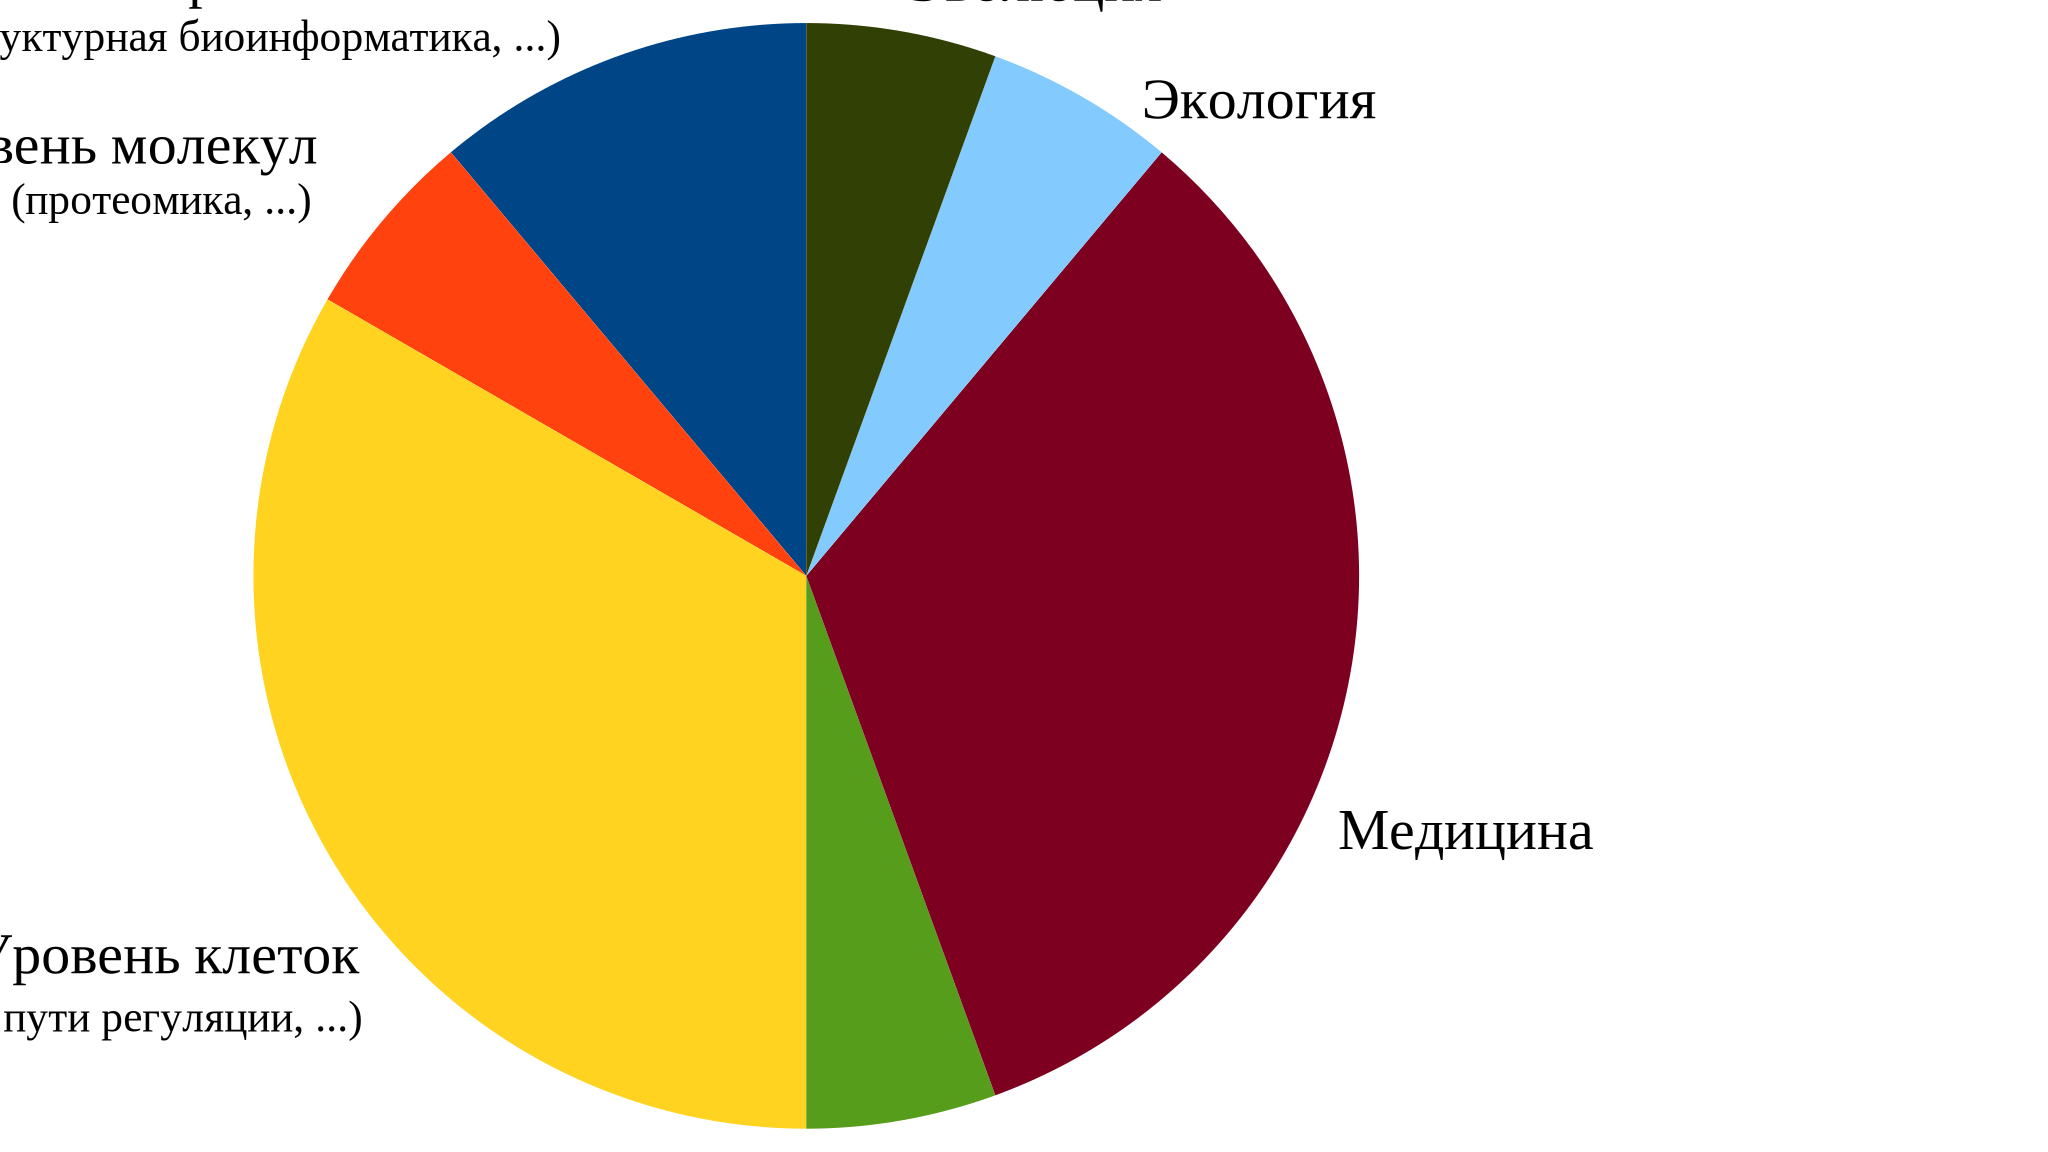
\includegraphics [width=0.8\linewidth]{pubmed_stats.png}
  \vskip 12pt
  \caption[m1]{
  \textbf{Интенсивность исследований в биомедицине}\itshape

Примерное разделение ресурсов между направлениям исследований, оцененное по количеству публикаций в базе биомедицинской литературы Pubmed за последнее десятилетие.

} 
 \label{img:pubmed_stats}
\end{figure}


Изучение систем регуляции клетки, по количеству исследований, развивается наиболее интенсивно, среди перечисленных направлений. Видимо, от этих исследований ожидается наибольшая практическая польза в приложениях к медицине. Потому молекулярные методы исследования клетки представлены в пособии лишь как краткий обзор, по причине быстрого развития методов и экспериментальных наблюдений в этой области. Статистические методы в медицинских приложениях также не раскрыты подробно в пособии, по причине быстрого развития этого направления и разнородности используемых методов и решаемых задач.


%Также здесь следует упомянуть о методах и пакетах программ, которые используются для восстановления структуры белков на уровне координат атомов


\section{Основные понятия молекулярной биологии клетки} \label{sect_molbio_notions}

\noindent
\textbf{ \textit{ДНК - "Дезоксирибонуклеиновая кислота" } } - молекула, по структурной химической формуле составленная, как цепь, из  однотипных \textit{нуклеотидных} остатков. Органические молекулы из класса \textit{дезоксирибонуклеотидов} содержат химическую группу (дезоксирибозу, из класса сахаров, и остаток фосфорной кислоты) и могут соединяться в цепь (полинулеотид) за счет образования ковалентной связи между фосфорной кислотой и дезоксирибозой смежного остатка. При этом, дезоксирибонуклеотиды различаются химической группой, ковалентно связанной с дезоксирибозой, и потому полинуклеотидная цепь ДНК может быть составлена из нескольких типов дезоксирибонуклеотидов, следующих в произвольном порядке.

В живой природе чаще всего встречаются цепи ДНК, составленные из четырех типов нуклеотидных остатков, обозначаемых обычно как A (Аденин), C (Цитозин), G (Гуанин), T (Тимин). Длина цепей ДНК может быть очень большой; в силу особенностей структуры дезоксирибинуклеотидов две цепи ДНК могут образовывать \textit{двойную спираль}. Структура двойной спирали является устойчивой, когда между смежными нуклеотидами в остатках двух цепей образуются водородные связи. Условием образования водородных связей является \textit{комплементарность} химических групп в смежных нуклеотидах: остаток аденина комплементарен остатку тимина, остаток цитозина комплементарен остатку гуанина.

\begin{figure}[H]
  \centering
  \vskip 12pt 
  \includegraphics [width=0.8\linewidth]{nucleotides.png}
  \vskip 12pt
  \caption[m1]{
  \textbf{Некоторые соединения - компоненты нуклеиновых кислот}\itshape

A - Рибоза, связанная с остатком фосфорной кислоты

B - Деоксирибоза, связанная с остатком фосфорной кислоты (Deoxyribose 1-phosphate)

C - Нуклеотид гуанозин (5'-Guanylic acid; Guanosine monophosphate). Гуанин - азотистое основание класса пуринов - соответствует химической группе в левой части молекулы. 

} 
 \label{img:nucleotides}
\end{figure}

К молекулам нуклеотидов, в первую очередь к аденозину и гуанозину, может быть добавлен еще один или два дополнительных остатка фосфорной кислоты. Реакция присоединения остатка фосфорной кислоты (\textit{фосфорилирование}) к нуклеотиду аденозину, и реакция его отщепления, происходящая с высвобождением энергии, часто используются при энергетическом обмене в клетке. Для обозначения нуклеотидов с дополнительными фосфатными группами, используются термины \textit{аденозиндифосфат (АДФ, ADP)} и \textit{аденозинтрифосфат (АТФ, ATP)}.

\noindent
\textbf{ \textit{РНК - "Рибонуклеиновая кислота" } } - молекула, по структурной химической формуле являющаяся полинуклеотидом подобным ДНК. \textit{Рибонуклеотиды}, из которых составлены молекулы РНК, отличаются от дезоксирибонуклеотидов дополнительным атомом кислорода в химической группе из класса сахаров. Потому по физико-химическим свойствам цепи РНК отличаются от цепей ДНК. Подобно цепям ДНК в живой природе, цепи РНК обычно составлены из четырех типов нуклеотидных остатков, и для цепей РНК также свойственно образование водородных связей между смежными комплементарными остатками. Но для молекулы РНК, комплементарные связи между цепями в двойной спирали менее устойчивы, чем комплементарные связи между фрагментами одной молекулы. 

\begin{figure}[H]
  \centering
  \vskip 12pt 
  \includegraphics [width=0.87\linewidth]{dnarna1.png}
  \vskip 12pt
  \caption[m1]{
  \textbf{Молекулы ДНК и РНК}\itshape

Слева: две цепи молекул ДНК, образующие двойную спираль. 

Справа: молекула РНК, в которой структура стабилизирована водородными связями между комплементарными нуклеотидами. 

\fontsize{11pt}{11pt}\selectfont
Изображены структуры ДНК и РНК (транспортная РНК tRNA-Gly), входящие в состав комплексов 6c1v и 4kr2. 

Направление цепей в полинуклеотидах показано с помощью ленты / трубки. Ароматические кольца в боковых цепях нуклеотидов в молекуле ДНК закрашены для большей наглядности. Четырьмя цветами обозначены четыре типа нуклеотидов.
Для визуализации был использован пакет VMD. 

} 
 \label{img:dnarna}
\end{figure}

Для обозначения некоторых типов молекул РНК, используются следующие термины:

\begin{itemize}

\item \textit{матричная РНК (мРНК, mRNA)} - молекула РНК, используемая как матрица, по которой при \textit{трансляции} в рибосомах синтезируется белок.

\item \textit{некодирующая РНК (ncRNA)} - молекулы РНК, синтезируемые в клетке, но не используемые для трансляции

\item \textit{транспортная РНК (тРНК, tRNA)} - молекула РНК (некодирующая), которая используется при синтезе белка. В молекулах тРНК, для которых характерна типичная трехмерная структура (рис. \ref{img:dnarna}), три нуклеотида используются для комплементарной связи с матричной РНК, а специфическая аминокислота, предварительно присоединенная к транспортной РНК, используется для продолжения цепи белка при синтезе.

\item \textit{микро РНК (miRNA)} - молекулы некодирующей РНК, которые участвуют в процессах регуляции процессов транскрипции и трансляции

\end{itemize}


\noindent
\textbf{ \textit{Белок} } - молекула, составленная, как цепь, из остатков молекул, относящихся к классу \textit{аминокислот}. В клетках используется 20 типов аминокислот (рис. \ref{img:dnarna}). Для белков в клетке характерно наличие устойчивой структуры, в которую уложена цепь аминокислотных остатков. В главе "Структурная биоинформатика" более подробно обсуждаются свойства белковых молекул и методы их анализа.

\begin{figure}[H]
  \centering
  \vskip 12pt 
  \includegraphics [width=0.99\linewidth]{protein.png}
  \vskip 12pt
  \caption[m1]{
  \textbf{Молекула миоглобина}\itshape

Белок миоглобин, в трех представлениях: 

Слева: полноатомная модель

В центре: главная цепь белка и молекула гема 

Справа: представление в виде ленточной диаграммы. Полупрозрачным показана поверхность, доступная растворителю


\fontsize{11pt}{11pt}\selectfont
Изображены структура окси-миоглобина 1a6m. 
Для визуализации был использован пакет UCSF Chimera. 

} 
 \label{img:protein}
\end{figure}

Некоторые из белков участвуют в катализе химических реакций в клетке; такие белки иногда называют \textit{ферментами} или \textit{энзимами (enzymes)}. Для коротких цепей аминокислот, не имеющих устойчивой укладки, используют термин \textit{пептид}.

\noindent
\textbf{ \textit{Метаболиты} } - низкомолекулярные химические соединения, с массой обычно менее 1 килодальтон, участвующие в биохимических процессах, происходящих в клетке (рис. \ref{img:metabolites}). В отличии от полинуклеотидов и белков, синтез метаболитов в клетке не задается непосредственно генетическим кодом. К метаболитам относятся продукты обмена веществ, гормоны и другие сигнальные молекулы, а также прочие низкомолекулярные соединения, как, например, лекарственные препараты. Иногда для обозначения низкомолекулярного соединения используют термин \textit{лиганд}, как, например, в контексте изучения катализа химической реакции белком-ферментом. В частности, молекула нуклеотида аденозинтрифосфата (АТФ) является лигандом многих ферментов, поскольку часто используется в энергетическом обмене клетки.

\begin{figure}[H]
  \centering
  \vskip 12pt 
  \includegraphics [width=0.8\linewidth]{metabolites.png}
  \vskip 12pt
  \caption[m1]{
  \textbf{Некоторые из химических соединений, участвующих в обмене веществ в организме}\itshape

Слева: молекула мочевины

В центре: молекула ацетилхолина 

Справа: молекула преднизолона


\fontsize{11pt}{11pt}\selectfont
Мочевина (urea) - конечный продукт метаболизма белка в клетке; ацетилхолин - один из нейромедиаторов; преднизолон -  синтетический лекарственный препарат, по структуре подобный гормонам, вырабатываемым корой надпочечников (кортикостероидам).

Для визуализации молекул был использован пакет UCSF Chimera. 

} 
 \label{img:metabolites}
\end{figure}


\noindent
\textbf{ \textit{Транскрипция} } - полимеризация молекулы РНК, происходящая посредством катализа в комплексе белков, с использованием молекулы ДНК в качестве шаблона.


\begin{figure}[H]
  \centering
  \vskip 12pt 
  \includegraphics [width=0.4\linewidth]{transcription.png}
  \vskip 12pt
  \caption[m1]{
  \textbf{Схема процесса транскрипции}\itshape
} 
 \label{img:transcription}
\end{figure}

Синтез РНК при транскрипции происходит на основании комплементарности очередного из остатков цепи шаблона и остатка, который добавляется в цепь РНК. Определение участка ДНК, на котором происходит транскрипция, происходит с участием белков, называемых \textit{транскрипционными факторами}, через связывание этих белков со специфическими участками молекулы ДНК. 


\noindent
\textbf{ \textit{Трансляция} } - полимеризация молекулы белка, происходящая посредством катализа в молекулярном комплексе, называемом \textit{рибосомой}, с использованием молекулы матричной РНК в качестве шаблона. В состав рибосомы, кроме молекул белка, входит несколько молекул некодирующей РНК (\textit{рибосомная РНК}), с характерной устойчивой пространственной укладкой.

\noindent
\textbf{ \textit{Метилирование ДНК} } - химическая модификация некоторых остатков цитозина в молекуле ДНК, состоящая замещении  водорода на метильную группы у атома C5 в ароматическом кольце цитозина. В ДНК клетки метилирование, как правило, происходит у остатков цитозина за которыми в цепи следуют остатки гуанина (C-G) и регулируется специфичными ферментами.

\noindent
\textbf{ \textit{Сплайсинг} } - модификация молекулы матричной РНК, происходящая посредством катализа в молекулярном комплексе, называемом \textit{сплайсосомой}. Модификация при сплайсинге состоит в вырезании определенных фрагментов матричной РНК и сращивании смежных участков РНК. Как результат, некоторые фрагменты ДНК, скопированные в процессе транскрипции в мРНК, выпадают на стадии трансляции мРНК в белок. Фрагменты ДНК, которые остаются в мРНК после сплайсинга и преобразуются во фрагменты белковой последовательности при трансляции, называются \textit{экзонами}, а участки ДНК, удаляемые из мРНК при сплайсинге, называются  \textit{интронами}.

\noindent
\textbf{ \textit{Пост-трансляционные модификации} } - общее название для процессов химической модификации некоторых аминокислотных остатков в белках, происходящих после синтеза белка в рибосоме. Некоторые пост-трансляционные модификации специфичны для отдельного белка или класса белков, некоторые - как, например, \textit{убиквитинирование}, регулируются универсальными ферментами. 

\noindent
\textbf{ \textit{Ген} } - термин, обозначающий "элементарную" единицу информации, закодированной в ДНК и проявляющуюся в наследственных свойствах организма. Своим возникновением связан с развитием \textit{генетики} в конце XIX - начале XX века. В молекулярной биологии термин используется, с долей условности, для обозначения фрагмента ДНК, с которого происходит транскрипция матричной РНК или некодирующей РНК, а также саму матричную / некодирующую РНК или белок, синтезируемый при трансляции матричной РНК. 

При учете \textit{экзон-интронной} структуры последовательностей ДНК, когда в результате \textit{альтернативного сплайсинга} одному фрагменту ДНК может соответствовать несколько мРНК, следует отличать термин \textit{ген} от термина \textit{изоформа}. В этом случае, для различения матричных РНК, а также белков синтезируемых при их трансляции, используют выражение \textit{изоформы гена}.

\noindent
\textbf{ \textit{Геном} } - термин, обозначающий совокупость наследственной информации, содержащейся в клетке. В большей части известных случаев, наследственная информация в клетке, к которой применимо понятие "геном", закодирована в молекулах ДНК, образующих молекулярные комплексы, которые можно заметить при достаточном увеличении как \textit{хромосомы} в ядре клетки. В многоклеточных организмах, как правило, один и тот же геном содержится во всех клетках организма.

Среди исключений из описания приведенного выше, следует упомянуть бактерии, в которых ДНК не образует хромосом, а также некоторые вирусы, в которых информация кодируется в молекуле РНК. Кроме того, митохондрии и хлоропласты, органеллы развивающиеся внутри клеток, содержат собственный генетический материал, дополняющий ДНК в хромосомах.

\section{Термины, используемые при постановке экспериментов и обработке данных} \label{sect_molbio_terms}

\noindent
\textbf{ \textit{Полимеразная цепная реакция (ПЦР, PCR)} } - экспериментальная методика, позволяющая многократно увеличить количество определенного фрагмента ДНК, при условии наличия этого фрагмента в биоматериале. Копирование фрагмента происходит при участии фермента ДНК-полимеразы, а специфичность при выборе фрагмента в эксперименте определяется парой так называемых \textit{праймеров} - полинуклеотидов с длиной около 10 - 20 оснований. 

\noindent
\textbf{ \textit{ДНК-микрочип (microarray)} } (\textit{micr}) - технология, позволяющая детектировать присутствие и/или количество определенных фрагментов ДНК в биоматериале, независимо в каждой из ячеек микрочипа. Использование технологии позволяет быстро и эффективно характеризовать состав ДНК, содержащейся в биоматериале.



%C1 - John Schmidt C2 - Abizar B1 - nasa B2 - Schutz B3  -  Zongli Luo zongli@mail.ubc.ca A1,A2,C3 - Eigenes Werk
%John Schmidt Rkalendar  Schutz Flickr Konrad Förstner Mangapoco Abizar Eigenes Werk, Roger Bumgarner  Zongli Luo zongli@mail.ubc.ca
\noindent
\textbf{ \textit{Секвенирование (sequencing)} } - экспериментальное определение последовательностей ДНК, содержащихся в биоматериале.

Постановка экспериментов по определению последовавательностей ДНК предложена в 1977 г. \parencite{Sanger_1977}. Идея, заложенная в этой постановке, продолжает использоваться в других экспериментах, но в истории развития секвенирования разделяют методы первого, второго и третьего поколения. Ко второму поколению методов относится использование приборов, называемых \textit{секвенаторами}, в которых автоматизированы адаптированные лабораторные методики, необходимые для определения ДНК. Первые из секвенаторов, секвенаторы второго поколения, получили название \textit{капиллярных секвенаторов}. В третьем поколении методов, эффективность автоматизированного секвенирования оказалось возможным существенно увеличить, при условии разделения ДНК в биоматериале на относительно короткие фрагменты. Термин \textit{олигонуклеотид} используется как синоним для понятия "фрагмент ДНК", но для олигонуклеотидов, определенных при секвенировании, используется более узкий термин \textit{рид} ("прочтение", \textit{read}).  

\begin{figure}[H]
  \centering
  \vskip 12pt
  \includegraphics[width=0.88\linewidth]{mbmethods.png} \\ 
  \vskip 12pt
  \caption[m1]{
  \textbf{Некоторые экспериментальные методы и инструменты, используемые в молекулярной биологии}\itshape

\fontsize{11pt}{11pt}\selectfont

\textbf{Вверху:} полимеразная цепная реакция осуществляется за счет циклических изменений температуры в реакционном сосуде, на каждом цикле происходит удвоение количества специфического участка ДНК между двумя праймерами.

\textbf{В центре:} фрагменты ДНК в биоматериале могут специфически связываться с ДНК-зондами в лунках микрочипа за счет эффекта гибридизации.  Количество связанного ДНК в ячейке микрочипа определяется по интенсивности флуоресценции ячейки.
 
\textbf{Внизу:} в методе секвенирования "по Сэнгеру", обрыв цепи при синтезе ДНК на каждой из четырех дорожек может происходить в положении одного из четырех возможных нуклеотидов. В первых экспериментах, для определения последовательности нуклеотидов использовался гель-электрофорез фрагментов ДНК разной длины, помеченных радиоактивной меткой.

\fontsize{10pt}{10pt}\selectfont
Авторство изображений: John Schmidt, Abizar, Schutz, WiWiki, kOchstudiO
} 
 \label{img:mbmethods}
\end{figure}


\noindent
\textbf{ \textit{Выравнивание (alignment)} } - комбинаторная задача и алгоритм расстановки вставок (\textit{gaps, гэпов}) в две или более последовательности символов, для достижения максимальной степени сходства между символами в одном столбце, при условии что с учетом вставок последовательности имеют одинаковую длину. В описанной постановке задачи, выравниванием называется также таблица символов, где последовательности с добавленными гэпами записаны как строки.

В приложении к биологическим последовательностям, белковым или нуклеотидным, алгоритмы выравнивания позволяют восстановить мутации, состоявшие в выпадении или вставке нуклеотидных остатков в ДНК. При этом обычно подразумевается, что сравниваемые последовательности генов имеют общий ген-предок, и разделение последовательностей за счет внесения мутаций произошло в течении эволюции или развития организма.

Построение оптимального \textit{парного выравнивания} последователей возможно, при условии задания степени сходства между символами в последовательностях. Время расчетов при построении такого выравнивания (\textit{алгоритмическая сложность}) пропорциональна произведению длин двух последовательностей. Но, из-за степени алгоритмической сложности в задаче построения \textit{множественного выравнивания}, оптимальное выравнивание трех и более последовательностей в большинстве случаев найти невозможно, и в алгоритмах решения этой задачи используются эмпирические приближения.

Также, термином "выравнивание" обозначают сам набор последовательностей с расставленными гэпами. Для наиболее точного сравнения последовательностей определенного класса часто важен опыт экспертов, или даже просто непредвзятый взгляд биоинформатика. Применение универсальных эмпирических алгоритмах множественного выравнивания может привести к неоптимальным результатам во многих частных случаях, и полученное выравнивание требуется корректировать вручную.

\noindent
\textbf{ \textit{Ассемблирование (assembly, сборка)} } - класс алгоритмов и программ для обработки ридов полученных при высокопроизводительном секвенировании, с целью восстановления последовательностей ДНК, содержащихся в исходном биоматериале.

Алгоритмы ассемблирования основаны на совмещении идентичных частей в ридах, представляющих смежные участки ДНК. Задача составления длинных цепочек из ридов сводится к задаче нахождения оптимального пути в графе. При нахождении пути в графе разделяют задачу  \textit{Гамильтона} (поиск пути без пересечения по вершинам) и задачу \textit{Эйлера} (поиск пути без пересечения по ребрам). В отличии от задачи Гамильтона, по оценкам вычислительной сложности задачи Эйлера возможен поиск оптимальных путей за приемлемое время, при объемах данных используемых для ассемблирования (100 гигабайт и более). При постановке задачи Эйлера в приложении к ассемблированию вводится понятие так называемого \textit{k-мера} (\textit{k-mer}) - фрагмента нуклеотида длиной от 21 до примерно 120, заведомо меньшей чем длина рида (от 50 до 250 и более); полученный граф, в котором k-меры соответствуют ребрам, называется \textit{графом де Бройна}. Однако при ассемблировании с использованием графа де Бройна, для используемой аппаратной платформы предьявлляются высокие требования к объему оперативной памяти, поскольку при нахождении пути Эйлера в непредсказуемом порядке используются все k-меры в исходных данных. 

Существуют некоторые методики постановки экспериментов для улучшения достоверности и длины полученных фрагментов ДНК, однако ошибки в данных, допускаемые при секвенировании, так же как и наличие мало различимых фрагментов ДНК в исходном биоматериале, ограничивают качество полученных при ассемблировании результатов.


\begin{figure}[H]
  \centering
  \vskip 12pt
  \includegraphics[width=0.9\linewidth]{mbcalcmethods.png} \\ 
  \vskip 12pt
  \caption[m1]{
  \textbf{Некоторые алгоритмы и методы биоинформатики}\itshape
  
  
Вверху слева: пример множественного выравнивания. Выровненные последовательности для наглядности разбиты на блоки длиной в 10 символов, и столбцы, в которых все остатки идентичны или сходны по молекулярной массе, выделены цветом. Вставки в выравнивании принято обозначать символом "-".

Вверху справа: принцип ассемблирования с использованием графа де Бройна.

Внизу: структурная аннотация фрагмента генома человека. Пометки иллюстрируют экзон-интронную структуру генома.

\fontsize{10pt}{10pt}\selectfont
при подготовке иллюстрации использован онлайн сервис "UCSC genome browser"

} 
 \label{img:mbcalcmethods}
\end{figure}


\noindent
\textbf{ \textit{Аннотирование (annotation, аннотация)} } - в узком смысле, задача, состоящая в идентификации генов в последовательности генома. В этой задаче выделяют \textit{структурную аннотацию} генов, где результатом является определение положения участков генома, для которых возможна транскрипция в РНК, а также сигнальных участков генома, регулирующих процессы транскрипции. Следующим шагом при анализе генома может являться \textit{функциональная аннотация}, когда для найденных генов составляются характеристики, описывающие их функцию и роль в клеточных процессах. 

В широком смысле, аннотацией биологических последовательностей или других объектов, изучаемых в молекулярной биологии, называют составление краткого описания характеризующего заданные объекты. Так, например, выделяют задачу по установлению ассоциаций между ключевыми словами из заданного набора и некоторыми фрагментами последовательностей в базе данных белков. Другим примером можно упомянуть проект Gene Ontology (онтология генов), где в базах данных записаны связи наименования генов с так называемыми \textit{онтологическими терминами}. Онтологические термины в рамках этого проекта группируются на три класса: \textit{биологический процесс}, \textit{молекулярная функция}, \textit{компонент клетки}.

\section{Молекулярные методы исследования клетки}

\subsection{Цели и направления при исследовании клетки}

Геном клетки или многоклеточного организма, как последовательность нуклеотидов, возможно восстановить, следуя подробно задокументированным методикам, включающим секвенирование, ассемблирование и аннотацию генов. Но задача "прочесть" текст генома, подобно тому как читают текст книги, является намного более сложной, и эта задача далека от решения, несмотря на объем информации, накопленный в молекулярной биологии. 

Интересы научных групп, занятых изучением клетки, определяются не только указанным общим направлением, но и разного рода прикладными задачами, которые оговорены при финансировании проводимых исследований. Но, несмотря на различия в направлениях и интересах ученых, для достижения взаимопонимания между ними при описании работы клетки, выработаны термины и понятия, которые позволяют согласованно описывать результаты их работы. Наиболее общие и широкие из этих понятий приведены ниже:

\noindent
\textbf{ \textit{Путь метаболизма (metabolic pathway)} } - система последовательных биохимических трансформаций молекул-метаболитов, происходящая с участием белков-ферментов. Некоторые специфические процессы преобразования метаболитов лежат в основе питания клетки клетки, а также используются при ответе клетки на воздействия внешней среды, как, например, в клетках бактерий происходит компенсация к действию антибиотиков.

\noindent
\textbf{ \textit{Путь регуляции (signaling pathway)} } - система последовательно взаимодействующих белков, с участием метаболитов, РНК и геномной ДНК. Обнаружено в некоторых случаях, что запуск взаимодействий в цепях такого рода происходит под действием определенных внешних факторов, приводя, как результат, к изменению состояния клетки, и составу ее РНК и белков.

\noindent
\textbf{ \textit{Регуляция транскрипции} } - система взаимодействия транскрипционных факторов со специфическими участками ДНК, в ходе которой происходит синтез дополнительных транскрипционных факторов, а также других белков и РНК. Цепи взаимодействий, запущенные в этой системе, приводят к адаптации клетки к специфическим условиям среды, а также к коррекции состояния клетки, существующей в составе многоклеточного организма.

\noindent
\textbf{ \textit{Сеть взаимодействия генов} } - представление системы взаимодействующих генов в форме графа, где узлы соответствуют генам, а ребра - взаимодействию между генами. Такое представление является интуитивно понятным, однако его возможно применить к описанию биологических систем лишь с большой долей условности.

Также, для согласования результатов разнородных экспериментов, в большей части научных публикаций используют наименования конкретных  путей регуляции, общих для многих организмов. Некоторые из этих терминов и наименований, а так же степень их отношения к реальности, упоминаются в материалах всех разделов этой главы.

\subsection{Анализ протеома клетки}  

%Эксперименты, основанные на использовании гибридизации, полимеразной цепной реакии (ПЦР), или секвенирования ДНК позволяют определить присутствие или даже количество нуклеотидных последовательностей в биоматериале. Но для полноценных исследований, касающихся биомолекул в живой клетке, необходимо также идентифицировать белки и метаболиты, содержащиеся в биоматериале. Но, хотя на уровне ковалентных связей белки и устроены, подобно ДНК, как цепочки однотипных остатков, эксперименты по идентификации белков возможны лишь с использованием методов масс-спектрометрии и некоторых других подходов, менее специфичных чем масс-спектрометрия.

Некоторые из многих функций белков в клетке - катализ химических реакций и преобразование метаболитов, поддержание целостности формы клетки и ее коррекция, регуляция перемещения молекул через клеточную мембрану, передача информации в форме сигналов вовне и внутрь клетки. И потому информация о составе белков в клетке (\textit{протеоме}) часто может существенно прояснить понимание происходящих там процессов. Методы современной органической химии позволяют анализировать материал клетки и состав метаболитов. Но для анализа белков клетки необходимо использовать подходы к проведению экспериментов и расчетов, дополняющие методы органической химии. 

%Матричные РНК в клетке обычно транслируются в белки, однако состав белков в клетке (\textit{протеом}) может являться предметом дополнительного изучения экспериментальными методами. 

Среди существующих подходов к экспериментам по протеомике, позволяющих с достаточной специфичностью определить состав белков, следует упомянуть иммунологические методы, такие как иммуноферментный анализ и вестерн-блоттинг, и методы масс-спектрометрии.
Известна также экспериментальная методика определения последовательности белка (так называемое "секвенирование по Эдману"), однако в современной протеомике этот метод используют нечасто, поскольку его оказывается непросто увязать с так называемыми "высокопроизводительными" (\textit{high throughput}) подходами к экспериментам по изучению клетки.

Специфичность при иммунологических методах достигается за счет механизмов специфичности иммунной системы. Так называемые \textit{антитела}, белки, вырабатываемые клетками иммунной системы, могут специфично связываться с белками чужеродного возбудителя инфекции (\textit{антигенами}). Антитело является комплексом из нескольких белковых цепей, и специфичность при взаимодействии антитела с антигеном достигается за счет наличия вариабельных частей в последовательностях белков, составляющих антитело.

%В основе методов масс-спектрометрии заложена возможность экспериментално определить отношение массы частицы к ее заряду, называемое иногда mZ. В масс-спектрометрах, величина заряда частицы ограничена значениями в несколько единиц элементарного заряда, и, после разрешения неоднозначности в выборе величины заряда, в результате измерений на масс-спектрометрах возможно с большой точностью рассчитать массы исследуемых молекул. 

В основе методов масс-спектрометрии заложена возможность экспериментально определить отношение массы частицы к ее заряду, называемое иногда mZ. Из уравнений электродинамики легко вывести, что заряженная частица в однородном магнитном поле будет совершать движение по круговой траектории, или спиральной траектории с постоянным шагом и радиусом спирали. В этом выводе, радиус спирали определяется отношением массы частицы к ее заряду, который и оказывается возможно измерить с большой точностью. В масс-спектрометрах, величина заряда частицы ограничена значениями в несколько единиц элементарного заряда, и, после разрешения неоднозначности в выборе величины заряда, в результате измерений на масс-спектрометрах возможно рассчитать массы исследуемых молекул. 

Методы масс-спектрометрии допускают их использование для "высокопроизводительного" определения состава белков в биологическом материале, как это схематично показано на рис. \ref{img:proteomics_concept}. Фракции в биологическом материале возможно разделить с  использованием \textit{хроматографии}, по степени подвижности отдельных молекул. На следующем шаге, для разделения белков на пептиды обычно используют ферменты, такие как \textit{трипсин}, который разрыв любой белковой цепи в местах, где встроены аминокислоты R (аргинин) и L (лизин). Разделение пептида на заряженные ионы происходит в масс-спектрометре, после чего возможно определить отношение M/Z для каждого иона.


\begin{figure}[H]
  \centering
  \vskip 12pt
  \includegraphics[width=0.7\linewidth]{proteomics_concept.png} \\ 
  \vskip 12pt
  \caption[m1]{
  \textbf{Идеализированное представление экспериментов по протеомике}\itshape
  
  По постановке эксперимента, пики от каждого из ионов, полученных при расщеплении пептида, позволяют однозначно идентифицировать этот пептид.
  
  Также, несколько идентифицированных пептидов из одного белка позволяют верифицировать выбор белка.
  
  В идеале, идентифицированные в эксперименте белки должны согласованно указывають на решение исследуемой задачи.
  
  } 
 \label{img:proteomics_concept}
\end{figure}

Пики, полученные при измерениях на масс-спектрометре, показывают значение массы молекул, содержащихся в материале. Однако одно и то же значение массы может соответствовать молекулам, различным по составу и по структуре. Последовательность пептида в схеме на рис. \ref{img:proteomics_concept} возможно идентифицировать лишь при согласованности положения пиков в измеренном спектре. И также, условием идентификации белков является согласованность в составе определенных на первом шаге пептидов.

Но измеренные спектры не всегда могут быть согласованными, как это показано на рис. \ref{img:tandem_ms}. Располагая информацией о составе белков в биологическом материале, и о принципе разделения белков на пептиды, при интерпретации спектра следует выбрать наилучший пептид, из числа возможных. Однако не всегда этот выбор является однозначным.

\begin{figure}[H]
  \centering
  \vskip 12pt
  \includegraphics[width=0.9\linewidth]{tandem_ms.png} \\ 
  \vskip 12pt
  \caption[m1]{
  \textbf{Неоднозначности при идентификации пептидов в масс-спектрометрии}\itshape
  
  Слева: пики, полученные при измерении спектра M/Z, могут быть отнесены как разным ионам, полученным при расщеплении разных пептидов.
  
  Справа: для уточнения идентификации пептидов используется база данных, содержащая возможные последовательности белков. Однако иногда этот набор белков слишком велик, чтобы допустить однозначный выбор.
  
  
  \fontsize{11pt}{11pt}\selectfont
  при подготовки иллюстрации были использованы пакеты программ SearchGUI, PeptideShaker, OpenMS, на основе данных, полученных при исследованиях байкальской губки.
  
  } 
 \label{img:tandem_ms}
\end{figure}

Для преодоления обозначенных проблем используют значительно более сложные и "ухищренные" постановки эксперимента. Среди приемов, используемых в этих экспериментах, следует упомянуть химические модификации отдельных аминокислот и использование атомов с другим молекулярным весом (\text{изотопов}). Такого рода возможности по изменению массы фрагментов и смещению положения пиков в спектре используют в этих исследованиях для дополнительной верификации и уточнения результатов. Однако нижняя граница вероятность ошибки при идентификации пептидов и белков в протеомике составляет примерно 1\%. И, как правило, при использовании методов протеомики для решения прикладных задач требуется согласование этих подходов с другими экспериментальными и расчетными методами (рис. \ref{img:proteomics}).


%При исследовании биоматериала клетки, определение массы некоторого белка крайне редко позволяет идентифицировать этот белок среди многих тысяч белков, содержащихся в клетке, и потому в протеомике используют значительно более сложные постановки эксперимента, обзор возможных подходов к этим экспериментам выходит за рамки курса. 

%При исследовании биоматериала клетки, определение массы некоторого белка крайне редко позволяет идентифицировать этот белок среди многих тысяч белков, содержащихся в клетке. И потому в протеомике используются значительно более сложные постановки эксперимента, обзор возможных подходов к этим экспериментам выходит за рамки курса. Но следует сказать, что даже при использовании в экспериментах по протеомике самого современного оборудования и программного обеспечения, для решения прикладных задач требуется согласование этих подходов с другими экспериментальными и рассчетными методами.

\begin{figure}[H]
  \centering
  \vskip 12pt 
  \begin{minipage}[ht]{0.39\linewidth}\centering
    \includegraphics[width=0.99\linewidth]{proteomics_1.png} \\ 
  \end{minipage}
  \hfill
  \begin{minipage}[ht]{0.59\linewidth}\centering
    \includegraphics[width=0.99\linewidth]{proteomics_2.png} \\ 
  \end{minipage}
  \vskip 12pt
  \caption[m1]{
  \textbf{Представление некоторых экспериментов с использованием масс-спектрометрии}\itshape

Слева: исследование мишеней препарата dabrafenib среди ферментов класса kinase. Темными оттенками показаны белки, среди которых  с большей достоверностью следует выбрать искомый белок-мишень.

Справа: визуализация сети взаимодействующих белков, для которых методами протеомики было обнаружено изменение концентрации в стареющей ткани сердца. Взаимодействия белков восстановлены на основании базы данных "String". 


\fontsize{11pt}{11pt}\selectfont
рисунки из статей \parencite{Pradke_2017,Holland_2014}  
} 
 \label{img:proteomics}
\end{figure}

Как следствие, полученные результаты часто имеют качественный характер, и могут быть использованы лишь как подсказка, для обозначения направлений при поиске ответов и решений прикладных проблем. Впрочем, методы, основанные на секвенировании ДНК, описанные ниже, где нижнюю границу вероятности ошибки в сравнимых постановках задач можно оценить примерно в 0.1\%, имеют такого же рода ограничения при их использовании, существенно не расширяя возможности по интерпретации данных в задачах прикладной молекулярной биологии.

\subsection{Обработка экспериментов по секвенированию при изучении процессов в клетке}

В исследуемом биологическом процессе участвуют ферменты, закодированные в ДНК как некоторые гены. Не все белки, закодированные в ДНК, присутствуют в каждой из клеток в организме, и относительное количество каждого из белков зависит от типа клетки и многих других факторов. Белки синтезируются в клетке в процессе трансляции мРНК, потому относительное содержание мРНК в клетке должно быть связано с содержанием белка, который кодирует эта мРНК. Транскрипция каждой из мРНК регулируется специфическим транскрипционными факторами, и потому регуляция биологических процессов в клетке будет выражаться в изменениях относительного содержания мРНК для определенных генов. 

Среди технологий, используемых в современных методы секвенирования, есть подходы к считыванию последовательностей молекул мРНК, содержащихся в клетке, в форме коротких фрагментов ("ридов"). В итоге возможно получить большие объемы данных, в форме наборов "ридов", причем соотношение между "ридами" примерно соответствует содержанию каждой из мРНК в исходном материале. При условии, что известны последовательности всех генов в геноме, которым могли бы соответствовать мРНК, содержащиеся в клетке, относительное количество каждой из мРНК можно оценить по количеству считанных "ридов", идентичных некоторому фрагменту последовательности исходного гена.

Для оценки уровня экспрессии мРНК, при обработке таких экспериментов следует провести сравнение последовательности каждого из считанных "ридов" с последовательностью генома, так чтобы идентифицировать ген, соответствующий этому "риду". В итоге, после обработки всех исходных данных, каждому из генов будет сопоставлено некоторое количество "ридов", как это показано на рис.\ref{img:rnaseq_alignments} на примере фрагмента гена рибосомной РНК и "ридов", полученных при секвенировании образцов байкальской губки.

\begin{figure}[H]
  \centering
  \vskip 12pt
  \includegraphics[width=0.7\linewidth]{rnaseq_alignments.png} \\ 
  \vskip 12pt
  \caption[m1]{
  \textbf{Расчет уровня экспрессии по данным секвенирования}\itshape
 
  \fontsize{11pt}{11pt}\selectfont
  данные из серии экспериментов с кодом PRJNA480194
} 
 \label{img:rnaseq_alignments}
\end{figure}

В описанной схеме расчетов предполагается, что для исследуемого организма заранее известна последовательность генома, с указанием положения кодирующих участков (генов). Последовательность генома человека получена и проанализирована в начале 2000-х годов, и с этого времени биологических видов, для которых получены последовательности геномов, становится все больше. Работа по определению последовательности генома для еще одного биологического вида может найти применение в исследовании функционирования клеток, в организме, относящемуся к этому виду.

Обсуждение алгоритмов и подходов, используемых для получения последовательности генома, не включено в материал, представленый в этой книге; эти алгоритмы лишь кратко упомянуты в таблице \ref{tab:rnaseq_tools}, среди групп алгоритмов, относящихся к обработке экспериментов по секвенированию. В таблицу также включен класс алгоритмов выравнивания, который обычно используют для проведения выравнивания ридов, где необходимым условием является ускоренное проведение расчетов, даже за счет снижения точности результата.


\begin{table}[htbp]
\caption{Типовые преобразования данных при обработке экспериментов по секвенированию}\label{tab:rnaseq_tools}
\begin{tabular}{|m{0.3\textwidth}|m{0.2\textwidth}|m{0.2\textwidth}|m{0.2\textwidth}|}
\hline
\textbf{Класс алгоритмов}&\textbf{Исходные данные}&\textbf{Результат расчетов}&\textbf{Некоторые из пакетов программ}\\
\hline
Ассемблирование генома&риды ДНК&фрагменты генома (контиги)&\textit{Abyss}, \textit{SoapDeNovo}, \textit{Spades}, ... \\
\hline
Аннотация генома&контиги&последовательности ДНК генов ("транскриптов")&\textit{Maker}, \textit{Augustus}, \textit{Prokka}, ... \\
\hline
Выравнивание ридов РНК и ДНК с контигами генома&контиги, риды&набор выравниваний&\textit{Bowtie}, \textit{BWA}, ... \\
\hline
Выравнивание ридов РНК с контигами генома&контиги, риды, аннотация&набор выравниваний&\textit{Tophat}, ... \\
\hline
Ассемблирование транскриптома&риды РНК&последовательности "транскриптов"&\textit{Trinityrnaseq}, ...\\
\hline
Выравнивание ридов с последовательностями генов&транскрипты, риды&набор выравниваний&\textit{Bowtie}, \textit{Usearch}, \textit{Blast}, ... \\
\hline
Выделение мутаций и полиморфизмов&набор выравниваний&позиции и свойства полиморфизмов&\textit{Samtools}, \textit{Vcftools}, \textit{GATK}, ... \\
\hline
Расчет уровня экспрессии генов&набор выравниваний, аннотация& таблица уровней экспрессии генов&\textit{Cufflinks}, \textit{RSEM}, ... \\
\hline
\end{tabular}
\end{table}

Список, представленый в таблице \ref{tab:rnaseq_tools}, показывает возможности и проблемы, встающие при необходимости исследовать функции клеток, на основании результатов секвенирования. Некоторые из проблем, которые могут привести к искажению результатов и требуют разработки дополнительных классов алгоритмов, подробнее описаны ниже.  

\begin{itemize}

\item Данные секвенирования могут содержать ошибки, а так же включения фрагментов вспомогательных последовательностей ДНК, используемых при проведении секвенирования. Проведение очистки и фильтрации является необходимым предварительным этапом при обработке "сырых" данных. При фильтрации данных используют вероятности ошибок считывания, оцениваемые, при проведении секвенирования, совместно с идентификацией каждого из нуклеотидов.

\item Для оценки уровня экспрессии генов, следует оценить степень покрытия гена "ридами". Методологические затруднения возникают при сведении воедино оценок уровней экспрессии генов с различающейся длиной мРНК, и с различающейся степенью однородности покрытия (рис. \ref{img:rnaseq_alignments}).

\item В многоклеточных организмах, кодирующая часть гена, представленная в мРНК как непрерывная последовательность, в геноме обычно разделена в геноме на фрагменты ("экзоны"). Это может создать затруднения при попытке сравнить "рид", полученный как участок мРНК, с последовательностью генома.

\item При разделении гена на экзоны, эти экзоны могут быть составлены в клетке в мРНК несколькими способами. По "ридам" мРНК, может оказаться затруднительным выбор верного варианта мРНК как комбинации экзонов ("изоформы"), и даже оценка суммарного уровня экспрессии гена.

\item Геном любого организма обычно содержит повторяющиеся участки (рис. \ref{img:rnaseq_coverage}). В частности, сразу несколько генов в геноме могут иметь общий участок. Это создает затруднения при оценке уровней экспрессии, когда выбор гена, при выравнивании с "ридом" мРНК, является неоднозначным.

\item Наличие повторяющихся участков и неоднозначностей в геноме является наиболее "узким" местом при попытках ассемблировать последовательности мРНК по считанным "ридам", и потому оценки уровня экспрессии по последовательностям ассемблированных транскриптов являются менее надежными, чем оценки, полученные при использовании последовательности генома.

\end{itemize}


\begin{figure}[H]
  \centering
  \vskip 12pt 
  \begin{minipage}[ht]{0.6\linewidth}\centering
    \includegraphics[width=0.9\linewidth]{rnaseq_coverage_tail.png} \\ 
  \end{minipage}
  \hfill
  \begin{minipage}[ht]{0.38\linewidth}\centering
    \includegraphics[width=0.9\linewidth]{rnaseq_coverage_zipf.png} \\ 
  \end{minipage}
  \vskip 12pt
  \caption[m1]{
  \textbf{Распределение повторяющихся участков в геноме}\itshape

\fontsize{11pt}{11pt}\selectfont
Слева: диаграмма степени покрытия фрагментов генома "ридами" ДНК. По горизонтальной оси - уровень покрытия, по вертикальной оси - доля участков с таким уровнем покрытия в геноме.

Правая сторона показанного распределения иллюстрирует распределение повторяющихся участков в геноме, так что при "рид" возможно выровнять на любой из этих участков.

Справа: диаграмма покрытия в преобразованных координатах, иллюстрирующая выполнение "степенного закона" для распределения повторяющихся участков. Понятие "степенного закона" обсуждается подробнее в разделе \ref{sect_fractalmodels}.

\fontsize{10pt}{10pt}\selectfont
Использован геном модельного растения Arabidopsis thaliana. Рисунки из статьи \parencite{Kuzmin_2019}  
} 
 \label{img:rnaseq_coverage}
\end{figure}

Геном каждого из организмов, и каждой из клеток, не вполне идентичен модельному геному биологического вида, используемому при проведении выравниваний "ридов". Различия в последовательности генома и каждого из "ридов", показанные на рис. \ref{img:rnaseq_alignments} как "мутации", могут быть объяснены по-разному, и использованы на следующих ступенях анализа данных, обсуждение которых, в основном, выходит за рамки этой книги. Для некоторых, идеализированных и согласованных, распределений частот встречаемости нуклеотидов в позициях (рис. \ref{img:rnaseq_variants}), появление наблюдаемых "мутаций" следует объяснять однозначно. Однако, при обработке реальных данных, для интерпретации распределений такого рода используют отдельный класс алгоритмов, также упомянутый в таблице \ref{tab:rnaseq_tools}.


\begin{figure}[H]
  \centering
  \vskip 12pt
  \includegraphics[width=0.6\linewidth]{rnaseq_variants.png} \\ 
  \vskip 12pt
  \caption[m1]{
  \textbf{Идеализированные распределения нуклеотидов в вариабельных позициях}\itshape
} 
 \label{img:rnaseq_variants}
\end{figure}

Затраты на проведение секвенирования достаточно велики, но во многих исследованиях достаточно измерить относительное изменение отдельных выбранных генов. Технология полимеразной цепной реакции (ПЦР) разработана для детекции мРНК заранее определенного гена.  Для отделения выбранной мРНК в этом методе используются специфичные олигонуклеотды - \textit{праймеры}. Модификация этой технологии, "ПЦР в реальном времени", позволяет также определить относительное количество мРНК. Этот метод может быть использован для измерения относительного уровня экспрессии определенного гена, наряду с методами измерения содержания соответствующего белка (рис. \ref{img:gene_expression_changes}).


\begin{figure}[H]
  \centering
  \vskip 12pt
  \includegraphics[width=0.6\linewidth]{gene_expression_changes.png} \\ 
  \vskip 12pt
  \caption[m1]{
  \textbf{Методы детекции изменений в экспрессии генов}\itshape
  
  Слева - схема измерения относительного содержания уровня мРНК, при удвоении количества молекул на каждом шаге температурного цикла в полимеразной цепной реакции (ПЦР).
  
  Справа - измерение относительного содержания белков по уровню специфических антител.
  
  \fontsize{10pt}{10pt}\selectfont
  Иcходные изображения: design-droide.com, статья \parencite{Won_2014}.
} 
 \label{img:gene_expression_changes}
\end{figure}

Идентификацию и оценку количества мРНК сразу для большого количества генов возможно провести также с использование так называемых \textit{микрочипов (microarrays)}. В этой технологии, количество мРНК в биоматериале оценивается на основании степени гибридизации специфичных фрагментов ДНК в ячейках микрочипа. Ошибки и искажения в этом подходе, в целом, выше, чем при использовании секвенирования, и результаты экспериментов по двум технологиям непросто соотнести между собой. Но результат эксперимента в обоих подходах возможно свести к таблице, содержащей относительные значения содержания мРНК для каждого из выбранных генов.


\subsection{Дифференциальная экспрессия генов}

Традиционная и интуитивно простая постановка эксперимента по сравнению нескольких групп клеток или тканей может быть использована для определения генов, которые участвуют в регуляции биологических процессов, связанных с разделением использованных групп образцов.  В экспериментах по измерению \textit{дифференциальной экспрессии}, искомый набор генов возможно оценить по таблице, содержащей уровень экспрессии генов для каждого из образцов, с использованием моделей статистики.

Распределение генов по уровню экспрессии, полученное после обработки эксперимента, показано на рис. \ref{img:rnaseq_mdplot}. Некоторые белки и соответствующие им гены представлены в клетке в большом количестве. Иллюстрации в разделе построены на основе обработки серии экспериментов по исследованию эпителия легких у больных бронхиальной астмой. И, в частности, белок ферритин, соответствующий гену FTL, оказавшимся одним из наиболее представленных генов в этом анализе, используются в клетке для накопления ионов железа.


\begin{figure}[H]
  \centering
  \vskip 12pt
  \includegraphics[width=0.6\linewidth]{rnaseq_volcano_mdplot.png} \\ 
  \vskip 12pt
  \caption[m1]{
  \textbf{Распределение генов по уровню экспрессии}\itshape
  
  использовано представление "md-plot" (mean-difference plot)
  
  по вертикальной оси - относительное количество каждого из генов в образце, в логарифмических координатах
  
  по горизонтальной оси - количество гена в образце, по отношению к среднему его количеству в серии образов, в логарифмических координатах.
  
  \fontsize{11pt}{11pt}\selectfont
  данные из серии экспериментов с кодом PRJNA252605
} 
 \label{img:rnaseq_mdplot}
\end{figure}

Наиболее важная из целей, стоящих при обработке используемой серии экспериментов - связать изменение экспрессии генов с фактом заболевания. Вариации в среднем уровне экспрессии генов в двух группах исследованных тканей показано на рис. \ref{img:rnaseq_mdplot} как разброс точек по горизонтальной оси.

Для наиболее представленных генов, различие в среднем уровне экспрессии между группами невелико, как это показано в верхней части распределения на рис. \ref{img:rnaseq_mdplot}. Но различие между отдельными образцами, внутри каждой из групп, для выбранных генов может быть существенным, как это показано на рис. \ref{img:rnaseq_heatmap}. И, в результате, следует сделать вывод о том что, хоть экспрессия генов, выбранных как наиболее представленные, может существенно изменяться в отдельных образцах, эти изменения никак не связаны с фактом заболевания. Такого рода рассуждения используется как основание для количественных оценок вероятности связи уровня экспрессии гена с разделением между группами образцов.


\begin{figure}[H]
  \centering
  \vskip 12pt
  \includegraphics[width=0.9\linewidth]{rnaseq_heatmap.png} \\ 
  \vskip 12pt
  \caption[m1]{
  \textbf{Гены с наибольшим уровнем экспрессии}\itshape
  
  использовано представление "тепловой карты" ("heatmap")
  
} 
 \label{img:rnaseq_heatmap}
\end{figure}

Достоверность связи экспрессии гена с разделением образов по группам лишь косвенно соотносится с различием в среднем уровне экспрессии в группах. Различие в среднем уровне экспрессии может быть случайным, если для гена характерно неоднородное распределение в образцах, независимо от их группировки. Но косвенное соответствие между достоверностью связи и усредненным различием уровня экспрессии проявляется в наличии двух пиков в представлении таблицы экспрессии, показанном на рис. \ref{img:rnaseq_volcano}.

\begin{figure}[H]
  \centering
  \vskip 12pt
  \includegraphics[width=0.6\linewidth]{rnaseq_volcano.png} \\ 
  \vskip 12pt
  \caption[m1]{
  \textbf{Схема определения различающихся генов}\itshape
  
  использовано представление "volcano chart"
  
} 
 \label{img:rnaseq_volcano}
\end{figure}

На рис. \ref{img:rnaseq_volcano} проиллюстрирован принцип выбора наиболее различающихся генов. Уровень экспрессии этих генов в каждом из образцов показан на рис. \ref{img:rnaseq_heatmap_significant}. Все эти гены представлены в клетке в относительно небольшом количестве. И, как обобщение опыта работы с данными такого рода, следует отметить, что наибольший интерес в сравнительном анализе представляют гены, которые представлены в среднем хоть и в малом количестве, но полностью отсутствующие в одной из групп. 

\begin{figure}[H]
  \centering
  \vskip 12pt
  \includegraphics[width=0.9\linewidth]{rnaseq_heatmap_significant.png} \\ 
  \vskip 12pt
  \caption[m1]{
  \textbf{Гены с наибольшей достоверностью различия}\itshape

} 
 \label{img:rnaseq_heatmap_significant}
\end{figure}

Достоверность разделения десяти лучших генов в приведенном примере составляет от $1 \times 10^{-4}$ до $5 \times 10^{-4}$. Если учесть, что полное количество генов при этом составляет около $3 \times 10^{4}$, степень разделения генов "балансирует" на грани недостоверности. Построение наиболее точных статистических моделей в пакетах и программах, используемых для исследований по дифференциальной экспрессии, начинается с моделей распределения покрытия ридов при выравнивании с геномом. Однако, даже на этом уровне, ожидаемое распределение не всегда соответствует обнаруживаемому при обработке эксперимента. И, в условиях "балансирования" на грани недостоверности, использование других статистических моделей привело бы к отделению другого списка генов, как наиболее различающихся между образцами. Эти замечания дают основание для проведения подробного обсуждения последствий возможных ошибок при изучении экспрессии генов.

%Методики постановки экспериментов, используемые для выяснения и уточнения связи генов с процессами в клетке, включают так называемые эксперименты по . В экспериментах по дифференциальной экспрессии определяется относительное количество мРНК в образцах, для всех известных генов в геноме клетки, или для некоторой их части. В такой интерпретации, , 

%Принятые подходы к обработке таблиц с количественным составом РНК в серии образцов состоят в обработке каждой из строк таблицы с помощью некоторых статистических моделей, параметрических или непараметрических, для оценки степени различия каждого из исследуемых генов. Более того, при таком анализе неявно принят ряд конвенций, касающихся используемых статистических моделей. Эти конвенции касаются использования традиционно принятых методов оценки параметров на основе скрытых марковских моделей, способов выбора единиц описывающих степень покрытия гена, и др. 

%В практических приложениях, результаты описанных экспериментов не всегда удается свести к идентификации четко определенной группы генов, позволяющих интерпретировать детали изучаемого биологического процесса. Как примеры результатов, на рисунке \ref{img:diffexp}, слева, показана выделенная в результате эксперимента с использованием микрочипов группа генов микроРНК (miRNA), которые с некоторой достоверностью участвуют в регуляции процесса отторжения органов при трансплантации. И, напротив, справа на рисунке \ref{img:diffexp} показан пример обработки эксперимента по секвенированию РНК (\textit{RNA-Seq}), когда трудно выделить группу генов, которые можно было бы отнести к регуляции процессов, характерных для исследуемого образца.


\subsection{Ошибки и погрешности при изучении экспрессии генов} \label{sect_expressionbiases}

При обработке экспериментов по секвенированию мРНК возникает достаточно много неоднозначностей, касающихся методов выравнивания и способов оценки уровня экспрессии. Некоторые из проблем, встающих при выборе метода обработки данных, описаны в предыдущих разделах. Но применение более точных расчетных методов для прояснения этих проблем не всегда оправдано. В живых клетках, используемых в серии измерений, всегда оказываются различия, не учтенные в постановке эксперимента, и эти различия ограничивает достоверность выводов о различии в уровне экспрессии любого выбранного гена.

Но если рассмотреть группу генов, и оценить достоверность совместного изменения уровня экспрессии генов в этой группе, значимость выводов о изменениях внутри группы может быть достаточно велика. И с этим можно связать распространение подхода по аннотации подобных экспериментов на основании сравнения уровня экспрессии в заранее заданных наборах генов. В системах аннотации, каждый из наборов генов обозначен терминами, общими для многих тем, изучаемых в молекулярной биологии, что создает предпосылки к взаимопониманию между учеными из разных научных групп.

%ECM1 extracellular matrix protein GGA3	golgi associated, gamma adaptin ear containing, ARF binding protein PLA2G4E	phospholipase A2, group IVE RCOR3	REST corepressor SFMBT1	Scm-like with four mbt domains ZNF331	zinc finger protein 331

%	GOTERM_BP_ALL primary metabolic process 3.9E-2 organic substance metabolic process 5.3E-2 metabolic process 6.7E-2
	
Однако возможно допустить существование разных способов группировки генов в наборы, и сам факт использования группировки приводит к увеличению достоверности утверждений в прикладных исследованиях. Потому, как может оказаться, некоторые из принятых способов группировки возникли по большей части по историческим причинам при развитии молекулярной биологии. И потому, возможно, некоторые понятия в языке общения молекулярных биологов имеют мало отношения к объективно существующим механизмам регуляции экспрессии генов.

Губка \textit{Amphimedon queenslandica}, модельный организм из класса губок, привлекает внимание ученых, как объект для изучения ранних стадий развития эмбриона, для сравнению с развитием других, более высокоорганизованных, организмов. На рис. \ref{img:gene_expression}, на примере трех серий экспериментов по изучению развития эмбриона губки \textit{Amphimedon}, проиллюстрирована неоднородность в уровне экспрессии генов в образцах из одной серии (A) и преимущества при использовании группировки генов (B). В этом примере, рассматривались группы генов, составленные на основе корреляции в уровне экспрессии, но без связи с заранее аннотироваными наборами из систем по анализу дифференциальной экспрессии.



%Животные сгруппированы в ~ 35 «фил», основанных на представлении о различных планах тела1–4. Морфологический и молекулярный анализ показал, что стадия в середине развития, известная как филотипический период, сохраняется среди видов в некоторых типах 5–9. Хотя эти анализы подтверждают их существование, филюмы также подвергались критике за отсутствие объективного определения и, следовательно, на основе произвольных групп животных10. Здесь мы сравниваем транскриптомы развития десяти видов, каждый из которых аннотирован к разному типу, с широким спектром жизненных историй и эмбриональных форм. Мы обнаружили, что у всех десяти видов развитие включает в себя сочетание ранней и поздней фаз экспрессии консервативного гена. Эти фазы связаны дивергентным «переходом в середине развития», который использует видоспецифичные наборы сигнальных путей и факторов транскрипции. Этот переход в середине развития перекрывается с филотипическим периодом, который был определен ранее для трех из десяти типов, что позволяет предположить, что транскрипционные цепи и сигнальные механизмы, активные во время этого перехода, имеют решающее значение для определения плана филетического тела и что переход в середине развития может быть используется для определения филотипических периодов в других типах. С учетом этих наблюдений наряду с сохранением среднего уровня развития в пределах типов, мы предлагаем определить тип как совокупность видов, экспрессия генов которых на переходном этапе среднего развития как высоко консервативна среди них, так и отличается по сравнению с другими видами.

\begin{figure}[H]
  \centering
  \vskip 12pt
  \includegraphics[width=0.88\linewidth]{gene_expression.png} \\ 
  \vskip 12pt
  \caption[m1]{
  \textbf{Группировка генов для интерпретации сравнительного анализа экспрессии}\itshape
  
\fontsize{11pt}{11pt}\selectfont


Сравнение экспрессии генов в трех стадии развития эмбриона губки Amphimedon queenslandica.

Расчет проведен по результатам обработки трех независимых серий экспериментов Rna-seq по изучению развития эмбриона губки. 

A. Тройная диаграмма, иллюстрирующая неоднородность профиля экспрессии генов в образцах, относящихся к одой стадии развития. Для диаграммы выбраны три гена, с наибольшим усредненным различием в уровне экспрессии при сравнении образцов по трем стадиям развития. 

B. Тройная диаграмма, иллюстрирующая возможности по упорядочению представлений о регуляции экспрессии, допустив что в некоторой группе генов  экспрессия изменяется согласовано. Для диаграммы выбрана группа из 60 генов, построенная с использованием подходов из теории графов. Выбор группы генов был основан на связи в уровне экспрессии генов в серии экспериментов, и на наиболее значимом разделении образцов по стадии развития.
 
Оценки статистической значимости разделения: по генам - $10^{-10}$, по группе - $10^{-30}$.

\fontsize{10pt}{10pt}\selectfont
Для расчетов была использована библиотека igraph и материалы, опубликованные в \parencite{Adamska_2007,Anavy_2014,Levin_2016}.
} 
 \label{img:gene_expression}
\end{figure}

Намерение ученых изучить механизмы развития с помощью современных методов молекулярной биологии понятно. Но результаты таких исследований, подобные опубликованным в работе \parencite{Levin_2016}, основанные на типовых методах аннотации экспрессии генов, с достоверностью не выше $10^{-3}$, не всегда добавляют существенно новую информацию для прояснения ответов на вопросы, мотивировавшие проведение исследований. И это добавляет сомнений о реалистичности картины мира в представлении современной молекулярной биологии. 


%Но тем не менее, в результате накопления опыта в исследованиях такого рода, были выработаны некоторые достаточно устойчивые, хотя и не вполне четко очерченные, представления и понятия о деталях устройства систем регуляции в клетках, и роли определенных генов в этой регуляции.



%Так, например, в используемых непараметрических моделях принято считать, что вероятность покрытия фрагмента генома определенным количеством ридов при таком анализе описывается так называемым \textit{отрицательным биномиальным распределением}. Функция вероятности выпадения $k$ ридов в этом распределении выражается формулой $F(k) = \frac{\Gamma( r + k )}{k!\Gamma(r)}p^r (1-p)^k$. Это распределение содержит два параметра $r$ и $p$, и используется как обобщение распределения Пуассона $F_p(k) = \frac{\lambda^k}{k!}e^{-\lambda}$. Среднее значение величины покрытия, необходимое для оценки количества РНК, будет равно $\lambda$ при использовании распределения Пуассона. Использование отрицательного биномиального распределения оправдывается необходимостью введение второго параметра для описания эффекта увеличения дисперсии, замечаемого в экспериментально рассчитанных распределениях. 


%Эти конвенции можно оправдать требованиями к воспроизводимости результатов, предъявляемых обычно к экспериментальным методикам. Однако недостаточное взаимопонимание между специалистами, выполняющими разные этапы исследования, также зачастую приводит к неоправданному использованию конвенций, и, в итоге, к невозможности интерпретировать результаты экспериментов в контексте требуемых прикладных задач.

%\subsection{Протеомика - краткие замечания}



\subsection{Исследование систем регуляции в клетке} \label{sect_cellsystems}

В основе систем регуляции клетки лежат факты взаимодействие белков и других биомолекул. Для восстановления принципов устройства систем регуляции клетки, возможно использовать результаты экспериментов, таких как эксперименты по дифференциальной экспрессии. При этом, результаты экспериментов следует "спроектировать" на какое-либо модельное представление систем регуляции. Среди упрощений, вводимых в таких моделях, следует назвать принцип попарного взаимодействия генов. Взаимодействие возможно на уровне белков, на уровне регуляции экспрессии гена при взаимодействии белка с ДНК, не говоря о разного рода вариантах и "исключениях из правил", которые возможно обнаружить при детальном анализе конкретных белков и механизмов их функционирования.

Проблемы, возникающие в задаче определения взаимодействующих генов, включают задачу отделения прямых взаимодействия от косвенных, и задачу отделения причин и следствий в наблюдаемых явлениях. Как можно пояснить эти проблемы на примере анализа дифференциальной экспрессии, по результатам обработки серии экспериментов по измерению состава транскриптома несложно заметить корреляцию в экспрессии некоторых генов. Но при этом остается открытым вопрос, связана ли наблюдаемая корреляция с фактом непосредственного взаимодействия генов, и, если факт взаимодействия был, то в каком направлении происходила регуляция.

Для уточнения фактов взаимодействия генов и направления регуляции клеточных процессов, разработано достаточно много подходов к постановке экспериментов и расчетов. Среди этих подходов, можно назвать методику постановки экспериментов по выяснению участков ДНК, являющихся мишенями для определенного транскрипционного фактора (\textit{"Chip-Seq"}), и методику по выяснению роли определенного гена в регуляции клетки, состоящие в подавлении его экспрессии в геноме (\textit{"Knockout\"}). Но более подробное перечисление возможных подходов выходит за рамки данного курса.

Как итоги усилий по исследованию механизмов регуляции клетки, были сформированы понятия о некоторых ключевых сигнальных путях, изменения в которых приводят к сбоям в развитии организма. На рис. \ref{img:developmental_pathways} показаны результаты экспериментов по сравнительному анализу механизмов развития в многоклеточных организмах, где для нахождения сходства и различий в развитии оценивалась степень экспрессии генов в наиболее исследованных сигнальных путях.

В белках из класса транскрипционных факторов необходимой является функция связывания с двойной спиралью ДНК. Лишь небольшое число укладок белка обеспечивает эту функцию, среди всех транскрипционных факторов в геноме. Если в гене с неизвестной функцией обнаружена гомология с одним из мотивов, характерных для транскрипционных факторов, это является основанием отнести этот ген по функции к транскрипционным факторам. Гены, отнесенные к транскрипционным факторам, с общим типом укладки также образуют группу. И уровень экспрессии генов в наиболее исследованных группах транскрипционных факторов также показана в сравнительном представлении на рис. \ref{img:developmental_pathways}.

\begin{figure}[H]
  \centering
  \vskip 12pt
  \includegraphics[width=0.8\linewidth]{developmental_pathways.png} \\ 
  \vskip 12pt
  \caption[m1]{
  \textbf{Результаты функциональной аннотации некоторых сигнальных путей и семейств транскрипционных факторов на разных стадиях развития эмбрионов}\itshape
  
  Показанные результаты использованы для аргументации оригинальной модели развития многоклеточных организмов, названной авторами "модель обратных песочных часов".

\fontsize{11pt}{11pt}\selectfont
Рисунок из работы \parencite{Levin_2016}.
} 
 \label{img:developmental_pathways}
\end{figure}

Обозначения сигнальных путей на рис. \ref{img:developmental_pathways} являются распространенными терминами в языке общения молекулярных биологов, как это показано на рис. \ref{img:pathways_biases}. И действительно, даже для одноклеточных организмов в их механизмах адаптации можно заметить сценарии поведения, по сложности сравнимые с поведением высокоразвитых животных в сообществе. Клетки могут защищаться от внешних угроз, могут находиться в состоянии стресса, могут совершать "суицид", могут менять стратегию адаптации. В многоклеточных организмах, кроме этих стратегий, многие из механизмов отвечают за организацию отношений с другими клетками. Все перечисленные выше сценарии в этих клетках запускаются согласованно с состоянием организма как целого. Кроме того, возможен переход клетки в состояние "злокачественной", что в итоге приводит к развитию раковой опухоли и гибели всего организма.

В кратком пересказе, обозначения сигнальных путей можно объяснить в этих же терминах. Термин NF-kB обозначает молекулярный комплекс, который активируется в состоянии воспаления. Термин TGF (tumor growth factor) относится к сигнальному пути, характерному при перерождении клетки в раковую. Термин Jak (Janus kinase) относится к сигнальному пути, который активируется при заражении клетки внешним патогеном (вирусом). Термин Wnt относится к группе сигнальных путей, регулирующих согласованность выбора стратегий в клетках при развитии организма. Более узкий термин Bmal1 относится к сигнальному пути, обеспечивающему периодичность процессов в организме, синхронную с астрономическим временем. 

Также здесь следует упомянуть термины TNF (tumor necrosis factor), относящийся к процессу \textit{апоптоза} - программируемой гибели клетки, p53 - белок, тормозящий процессы переключения клетки в режим злокачественного развития, и CD4 - рецептор клеток иммунной системы, участвующий в системе различения здоровых клеток своего организма от чужеродных и зараженных клеток. Перегибы в росте числа публикаций, в которых упоминаются эти термины (рис. \ref{img:pathways_biases}), иллюстрируют изменчивость интересов исследователей при развитии этой области знаний.

%from 2013, "expression" - 685386, +wnt 12051, +tgf 16521, +notch 5044 +mapk 15675 +jak, 3139 +NF, 28780 +bmal1 810

\begin{figure}[H]
  \centering
  \vskip 12pt
    \begin{minipage}[ht]{0.57\linewidth}\centering
    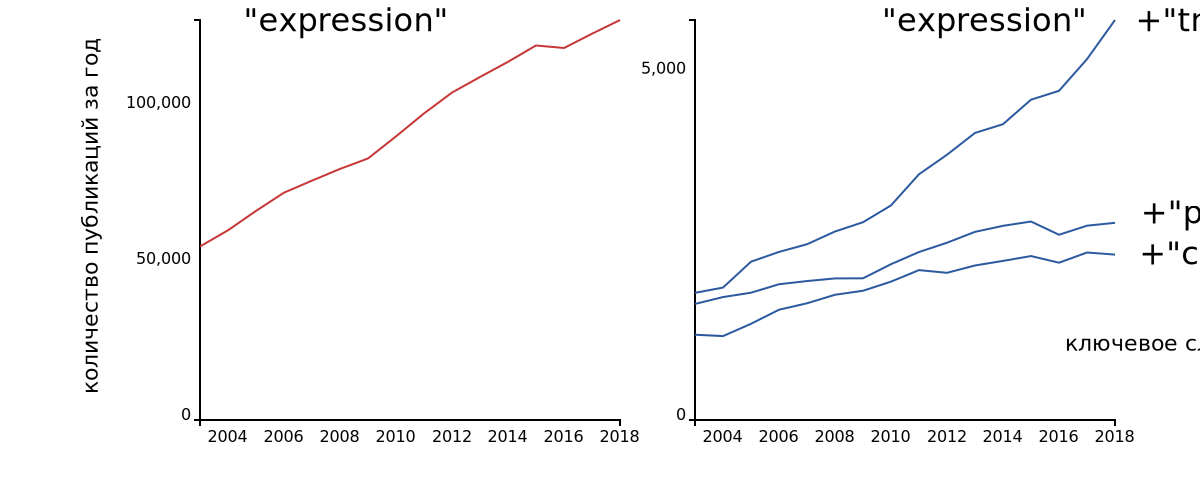
\includegraphics[width=0.99\linewidth]{pathway_terms_dynamics.png} \\ 
  \end{minipage}
  \hfill
  \begin{minipage}[ht]{0.4\linewidth}\centering
    \includegraphics[width=0.99\linewidth]{pathway_terms.png} \\ 
  \end{minipage}\\
  \vskip 24pt
  \includegraphics[width=0.35\linewidth]{human_lymphocyte.jpg} \\ 
  \vskip 12pt
  \caption[m1]{
  \textbf{Иллюстрация к обсуждению возможных систематических ошибок в языке общения молекулярных биологов}\itshape
  
  Вверху справа: Относительная частота упоминаний терминов, относящихся к обсуждению сигнальных путей, в библиографиях базы Pubmed, с 2013 года.
  Как фон, показано полное количество публикаций с упоминанием термина "экспрессия" за это время, около 700 тыс.

  Вверху слева: Рост числа публикаций с упоминанием названий некоторых ключевых генов.
  
  Внизу: Лимфоцит человека, одна из клеток иммунной системы. Изображение получено методом сканирующей электронной микроскопии, в 1976 году.

\fontsize{11pt}{11pt}\selectfont
Credits: NCI
} 
 \label{img:pathways_biases}
\end{figure}

Но, в геномах многоклеточных организмов закодировано обычно более 30 тыс. генов, и при условии их изучения, соразмерного с их ролью в регуляции клетки, относительная представленность названий этих генов в научных публикациях находилась бы на уровне не выше чем для гена BMAL1 на рис. \ref{img:pathways_biases}. И, возможность переоценки и смещения акцентов в интерпретации экспериментов была показана выше, при обсуждении методов обработки измерений дифференциальной экспрессии генов. Потому, характерные черты краткого список терминов, используемых для обозначения сигнальных путей, могут лишь укрепить сомнения в адекватности языка общения молекулярных биологов.

Возможность количественных оценок значимости, безусловно, привлекает к использованию подходов по обработке экспериментов, основанных на таких оценках. Но для сложно устроенной системы регуляции в клетках, статистические модели, используемые для получения этих оценок, могут вносить существенные искажения в результаты. И также, выбор методов и технологий обработки данных в каждом из прикладных исследований может быть не всегда наилучшим. Смещения акцентов при этом выборе могут возникнуть так же как и смещения акцентов при анализе систем регуляции. Но, несмотря на указанные недостатки, следует обратить внимание на "здоровое начало", содержащееся в обширных данных, накопленных при изучении систем клетки.

Большая часть ошибочных интерпретаций возникает при обработке экспериментов, при попытках сократить и обобщить полученные данные. Но, по принятой в современной науке традиции, "сырые данные" экспериментов также часто остаются доступными, допуская возможность их обработки с использованием других подходов. Если эксперимент был поставлен с целью проверки заведомо неадекватной гипотезы, эти данные являются мало полезными. Но все же, если даже считать уровень измеренного в эксперименте гена из семейства JAK не имеющим прямого отношения к системе защиты клетки, как это предполагалось при постановке эксперимента, эта информация также может найти применение в более широком сводном анализе.

\begin{figure}[H]
  \centering
  \vskip 12pt
  \includegraphics[width=0.6\linewidth]{gene_network.png} \\ 
  \vskip 12pt
  \caption[m1]{
  \textbf{Пример сравнения сетей регуляции генов}\itshape
  
Слева - клеточные линии раковых опухолей; справа - здоровые ткани

Вверху - сравнение сетей регуляции для клеток крови

Внизу - сравнение сетей регуляции для клеток кожи

Светлыми прямоугольниками обозначены транскрипционные факторы, темными кружками - гены-мишени транскрипционных факторов. Цветовая интенсивность линий в графе показывает степень зависимости между элементами графа. 

\fontsize{11pt}{11pt}\selectfont
рисунок из статьи \parencite{LopesRamos_2017}. 

Ссогласно содержанию статьи, связи в графе установлены на основе обработки экспериментов по измерению экспрессии генов, и частично проверены по результатам экспериментов Chip-Seq.


} 
 \label{img:gene_network}
\end{figure}

Пример такого сводного анализа приведен на рисунке \ref{img:gene_network}, где показан результат сравнения сетей регуляции генов в здоровых клетках, и в клетках, переродившихся в раковые. На рисунке заметно качественное различие в количестве взаимодействий, связывающих гены в процессах регуляции. Можно допустить также и другие способы сводного анализа, позволяющие на качественном уровне обобщить данные экспериментов. Но, поставив под сомнение количественные способы расчетов, нет оснований отдавать преимущества качественным оценкам, где заведомо нет возможности оценить достоверность выводов. Можно лишь с неизбежностью сделать вывод о том, что смысл и основание исследований в молекулярной биологии, в том числе исследований систем клетки, следует искать вне молекулярной биологии.


%\noindent \textbf{ \textit{Апоптоз} } - регулируемый процесс программируемой клеточной гибели. На молекулярном уровне, процесс состоит в каскаде реакций, заканчивающихся разрушением клетки. Сигнальные пути апоптоза запрограммированны в геноме клетки, и его инициация  может происходить на основании внешних или внутриклеточных факторов. В конечной фазе каскада реакций, происходит разрыв мембраны митохондрий и, затем, клетка распадается на отдельные органические "тельца". Известны некоторые белки и гены, участвующие в реакциях в касаде апоптоза, среди них - белок TNF ("tumor necrosis factor", фактор некроза опухолей), рецепторы, воспринимающие сигнал апопотоза, и ферменты, разрушающие структуру клетки.


% апоптоз интерферон стресс
%Сигнальный путь Wnt — один из внутриклеточных сигнальных путей животных, регулирующий эмбриогенез, дифференцировку клеток и развитие злокачественных опухолей
%Wnt signaling pathways use either nearby cell-cell communication (paracrine) or same-cell communication (autocrine). They are highly evolutionarily conserved in animals, which means they are similar across animal species from fruit flies to humans.[3][4]

%Wnt signaling was first identified for its role in carcinogenesis, then for its function in embryonic development. The embryonic processes it controls include body axis patterning, cell fate specification, cell proliferation and cell migration. These processes are necessary for proper formation of important tissues including bone, heart and muscle. Its role in embryonic development was discovered when genetic mutations in Wnt pathway proteins produced abnormal fruit fly embryos. Wnt signaling also controls tissue regeneration in adult bone marrow, skin and intestine.[5] Later research found that the genes responsible for these abnormalities also influenced breast cancer development in mice.

%This pathway's clinical importance was demonstrated by mutations that lead to various diseases, including breast and prostate cancer, glioblastoma, type II diabetes and others.[6][7] Encouragingly, in recent years researchers reported first successful use of Wnt pathway inhibitors in mouse models of disease


%The JAK-STAT signalling pathway is a chain of interactions between proteins in a cell, and is involved in processes such as immunity, cell division, cell death and tumour formation. The pathway communicates information from chemical signals outside of a cell to the cell nucleus, resulting in the activation of genes through a process called transcription. There are three key parts of JAK-STAT signalling: Janus kinases (JAKs), Signal Transducer and Activator of Transcription proteins (STATs), and receptors (which bind the chemical signals).[1] Disrupted JAK-STAT signalling may lead to a variety of diseases, such as skin conditions, cancers, and disorders affecting the immune system.

%Inappropriate activation of NF-κB has been associated with a number of inflammatory diseases while persistent inhibition of NF-κB leads to inappropriate immune cell development or delayed cell growth

%Транскрипцио́нный фактор NF-κB (ядерный фактор «каппа-би»; англ. nuclear factor kappa-light-chain-enhancer of activated B cells, NF-kB) — универсальный фактор транскрипции, контролирующий экспрессию генов иммунного ответа, апоптоза и клеточного цикла. Нарушение регуляции NF-kB вызывает воспаление, аутоиммунные заболевания, а также развитие вирусных инфекций и рака. Семейство NF-kB состоит из 5 белков: NF-kB1 (или p50), NF-kB2 (или p52), RelA (или p65), RelB и c-Rel, образующих 15 комбинаций димеров. Все белки семейства объединяет наличие домена гомологии Rel, который обеспечивает образование белковых димеров, связывание NF-kB с ДНК и с цитозольным ингибиторным белком IkB. Фактор NF-kB проявляет активность только в димерной форме (возможно образование как гетеро-, так и гомодимеров), причём наиболее распространённые формы — димеры субъединиц p50 или p52 с субъединицей p65.

%NF-kB активируется целым рядом стимулов, включая цитокины (такие как TNF и интерлейкин 1), T- и B-клеточные митогены, бактериальные и вирусные продукты (все лиганды толл-подобных рецепторов, например липополисахарид или двухцепочечная вирусная РНК) и факторы стресса (такие как реактивные формы кислорода или ультрафиолет). В цитоплазме клетки NF-kB находится в неактивном состоянии в комплексе с ингибиторным белком IkB. Стимулирующий агент активизирует сигнальный путь NF-κB, при этом IkB фосфорилируется под действием киназы IKK (IkB-киназа), что приводит к деградации IkB в результате действия 26S протеасомы. При этом NF-kB высвобождается от ингибирующего комплекса, транслоцируется в ядро и активирует транскрипцию контролируемых генов.

%У млекопитающих главными генами, лежащими в основе циркадианного молекулярного осциллятора супрахиазматического ядра гипоталамуса, являются гены mPer1 и mPer2 («m» означает «mammalian», то есть period-ген млекопитающих). Экспрессия mPer1 и mPer2 регулируется транскрипционными факторами CLOCK и BMAL1. Гетеромеры CLOCK/BMAL1 связываются с промоторами генов mPer1 и mPer2, что инициирует их транскрипцию. Образующиеся в результате этого мРНК транслируются в цитоплазме клеток супрахиазматического ядра в белки mPER1 и mPER2. Эти белки проникают в ядра клеток и, будучи теперь уже связанными с белками mCRY1 и mCRY2, подавляют транскрипцию генов mPer1 и mPer2, связываясь с CLOCK/BMAL1-белками. Таким образом, по механизму отрицательной обратной связи формируется чередование подъёмов и спадов продукции мРНК, а затем и самих белков mPER1 и mPER2 с фазой, равной приблизительно 24 ч. Этот цикл подстраивается под ритм освещенности[7].

%Существует несколько дополнительных молекулярных циклов, регулирующих циклическую экспрессию генов mPer1 и mPer2. Белок BMAL1 тоже синтезируется циклически, и его продукция находится в противофазе с ритмом экспрессии генов mPer1 и mPer2. Транскрипция гена Bmal1 индуцируется белком mPER2 и тормозится белком REV-ERBα. В промоторах генов Cry1 и Cry2 содержится та же нуклеотидная последовательность (Е-box), что и в промоторах генов mPer1 и mPer2, поэтому транскрипция генов Cry1 и Cry2 позитивно регулируется комплексом CLOCK/BMAL1. То же самое справедливо и для транскрипции гена Rev-Erbα[7].
\section{Аннотация и анализ публикаций}

\subsection{Подходы к автоматическому анализу текстов} \label{sect_computationallinguistics}

Языки, на которых общаются люди, имеют иерархическую структуру. При осмыслении и исследовании законов общения между людьми, возникли понятия "буква", "слово" и "предложение", чтобы обозначить наиболее устойчивые и независимые уровни, в общем объеме иерархически организованной информации. Но не любая иерархически организованная информация будет нести смысл при общении, так чтобы намерение того, кто передает сообщение, стало бы понятно.

Внутри традиций изучения каждого из языков, были выработаны правила, по которым буквы составляются в слова, и слова составляются в предложения, чтобы отличать бессмысленные сочетания слов от тех, которые, возможно, несут смысл. Но когда возникла необходимость обрабатывать тексты автоматически, при разработке программ и информационных систем, помимо использования жестких условий, разделяющих правильные или неправильные сочетании слов, получил развитие и другой подход, основанный на методах статистики.

Модели и алгоритмы, разрабатываемые для автоматического анализе текстов, возможно использовать только после проведения тестов и подбора параметров. Для подбора параметров моделей обычно используют большие объемы сходных по содержанию текстов, такую подборку текстов называют "корпус" (\textit{corpus}). В этом контексте, набор библиографических записей с кратким описанием результатов научных исследований по биомедицинской тематике, доступный через проект Pubmed, следует считать одним из "корпусов" текстов.

При автоматической обработке научных публикаций из базы Pubmed, при обработке каждой из записей сопоставляют изложенные там результаты с некоторыми вариантами шаблонных утверждений или фраз, когда поиск информации, которую возможно выразить через одно из этих шаблонных утверждений, поставлен как цель при проведении обработки всего "корпуса". В этом контексте, поиск публикаций по ключевым словам - наиболее простой из примеров автоматической обработки, когда шаблоном является просто определенный термин. 

В системе Pubmed, в "штатном" режиме работы, поиск информации происходит во взаимодействии с пользователем, читателем, который получает возможность увидеть подборку текстов, найденную по заданному ключевому слову, так чтобы самому понять смысл каждого из заголовков и выбрать среди найденных публикаций ту необходимую ему информацию, которую затруднительно записать как формальный шаблон. Но возможности человека понимать тексты по отдаленно знакомой ему тематике ограничены, и все большее применение находят результаты исследований, где результаты основаны полностью на автоматической обработке большого количества текстов, большую часть из которых никто из людей, участвующих в исследовании, не прочитывает.

В таком режиме, чем сложнее шаблон утверждения, заданный при поиске, тем больше вероятность пропустить нужную информацию, а также ошибиться, предположив наличие искомого утверждения в тексте, где его не содержится. Для фильтрации второго рода ошибок, следует использовать универсальные подходы к автоматической обработке текстов, включая проверку условий и правил, а также статистические модели.

\begin{figure}[H]
  \centering
  \vskip 12pt
  
\includegraphics[width=0.6\linewidth]{computational_linguistics.png} \\ 
  \vskip 12pt
  \caption[m1]{
  \textbf{Иллюстрация подходов при анализе текстов}\itshape
  
  Приведенные примеры предложений подобраны в базы библиографий Pubmed; были использованы публикации \parencite{Yao_2019,Nazıroğlu_2014}.
} 
 \label{img:computational_linguistics}
\end{figure}

На рисунке \ref{img:computational_linguistics}, в первом из примеров, фраза содержит сразу три ключевых слова. Hypericum - это латинское родовое название лекарственного растения, известного как "зверобой". Также, в этой фразе содержится название заболевания (depression), и обозначение химического соединения (hypericin). Шаблонное утверждение, которое соответстует подобранной фразе, состоит в том, что зверобой может использоваться как средство для лечения депрессии. 

Содержащееся в приведенной фразе название химического соединения могло бы быть использовано для составления других шаблонных утверждений, однако это название не используется непосредственно в установленной связи между наименованием растения и заболеванием. Но, для исключения неверно установленных связей, возможно учитывать особенности используемого "корпуса" текстов. Среди текстов, где одновременно упомянуты и название растения, и термин, обозначающий заболевание, доля ложных соответствий была бы велика. Однако, в рамках неявно принятых в научном сообществе конвенций о проведении исследований, касающихся эффекта лекарственных растений, и описании их результатов, упоминание какого-либо химического соединения в тексте относит этот текст ближе к рамкам этой конвенции. И требование о наличии названия какого-либо химического соединения в тексте позволяет уменьшить долю ложных соответствий, в описанной постановке задачи анализа текстов.

Второй из примеров на рис. \ref{img:computational_linguistics} иллюстрирует подход к решению задачи по анализу текстов, когда шаблоном поиска является утверждение об изменении экспрессии некоторого гена, в экспериментах по изучению эффекта лекарственных растений. В этой задаче, для исключения достаточной части ложных совпадений, и для определения направления изменения экспрессии, следует учитывать иерархическую структуру текстов. Порядок слов устанавиливает структуру внутри предложения, как это помечено на рис. \ref{img:computational_linguistics} тонкими стрелками. В общем случае, для восстановления смысла текста до необходимой степени, следует учитывать и другие отношения между словами. Так, в частности, использование отношения между местоимением it (он) и названием растения (hypericum) необходимо для достоверного восстановления содержащегося в тексте утверждения об эффекте, проявляющемся на уровне экспрессии генов.

Во втором из описанных подходов, вид ошибок, когда верная информация остается пропущенной при автоматической обработке, легко пояснить, выделив в этом подходе задачу поиска в тексте слов и фраз, использованных авторами для обозначения генов. Геномы многих модельных организмов, используемых при проведении экспериментов, содержат сходные наборы генов, и для согласованности при представлении результатов исследований, для сходных генов в разных организмах принято выбирать одинаковые идентификаторы. Но в каждой из статей, право выбрать термины для обозначения генов остается за авторами. И даже в публикациях, касающихся исследования наиболее "популярных" путей регуляции, о которых упомянуто в разделе \ref{sect_cellsystems}, названия генов можно записать по-разному. Например, гены, относящиеся к молекулярному комплексу NF-kB, можно обозначить как NF-kappaB, или NF-κB. И, поскольку генов в публикациях упоминается достаточно много, и в публикациях, где упоминаются названия некоторых генов, авторы зачатую выбирают различные варианты обозначения, то даже для проведения расчетов на наиболее простом из уровней иерархии, объем работ по подготовке  и проведению автоматического анализа текстов является существенным.  


\subsection{Ошибки в аннотации, причины и механизмы их накопления} \label{sect_annotationbiases}

Термин "онтология" относится к философии, науке о знании, и постановка задач аннотации в биоинформатике, в широком смысле, смыкается с задачей об упорядочении и "осмыслении" знания, накопленного в молекулярной биологии. Одна из наиболее очевидных проблем, возникающая при попытках найти решение этой глобальной цели, и проявляющаяся в задачах аннотации - это неполная достоверность некоторых результатов, лежащих в основе восстанавливаемой философской системы. Проведение функциональной аннотации генов проводится на основании сравнения неизвестных генов с эталонными базами данных, где содержатся биологические последовательности с подробными и проверенными описаниями. И, когда в некоторых из таких описаний закрадываются ошибки, что неизбежно при научных исследованиях, некоторые из этих ошибок многократно копируются при составлении функциональной аннотации других геномов. И потому к результатам по аннотации следует относиться с долей условности, и выводы, полученные из этих результатов, часто требуют дополнительных обоснований.

Научное сообщество - это часть общества, и заблуждения в науке подобны заблуждения в обществе. В обществе возможно социальное неравенство, и значительное социальное неравенство может отражать несправедливое устройство общества. Подобно этому, в современной науке некоторые из направлений исследований прорабатываются значительно подробнее чем остальные, и это может означать наличие ошибок в системе научного знания, более масштабных, чем упомянутые выше ошибки аннотации.

Ранее в истории, некоторые из результатов полученных на основе научного метода, привели к существенному расширению возможностей человека и общества, в военном деле, а так же промышленности, экономике, медицине, сельском хозяйстве. И потому, в современном обществе, если целью его движения "вперед" является стабильный рост "валового внутреннего продукта", измеряемого в денежном эквиваленте, одним из приоритетных направлений для достижения цели следует считать проведение научных исследований. Результатами работы научных групп являются законченные и опубликованные исследования, и степень эффективности ресурсов общества, выделенных на науку, можно оценить по количеству научных публикаций. Описанный механизм объясняет рост информации, доступной научному сообществу, в формате публикаций и в других видах.

Но, возможность человека упорядочить поток информации ограничены. И, имея способность к самовоспроизведению и находясь не вполне под контролем, информация иногда начинает "жить своей жизнью". И, через такого рода механизмы, при распространении информации проявляются черты конкурентной борьбы и существенного преимущества некоторых "видов". В условиях кризиса всего общества, преимущество "победителей" возрастает, по отношению к более "слабым", в том числе и в отношении приоритетных направлений исследования, и в отношении научных работников. 

При любого рода самовоспроизводстве фрагментов информации необходимыми являются затраты энергии. Источником энергии при копировании "видов" информации является та же энергия Солнца, которая питает и все живое. При описании цепочки передачи энергии в современной науке, следует упомянуть систему финансирования научных проектов, и вопрос о разделении прикладных и фундаментальных тем исследований.

В качестве примера, проиллюстированного на рис. \ref{img:proteinfolding_pubmed}, можно привести сравнительную динамику количества публикаций в базе Pubmed, по запросам "protein folding" и "protein folding amyloid". Исследование механизмов сворачивания белка, на которых основаны все процессы более высокого уровня в молекулярных системах, следует безусловно отнести к фундаментальным темам биофизики. И, одной из частных задач в этой обширной теме является исследование механизма образования \textit{амилоидных бляшек} (amyloid fibrils), накопление которых со временем привести к старческому слабоумию (\textit{болезни Альцгеймера}). Один из генов в геноме человека кодирует пептид, для которого возможно два устойчивых варианта конформации. Один, "неверный", вариант конформации обладает свойством к самовоспроизведению, так что количество "неверно" свернутых пептидов возрастает. Такие "неверно уложенные" пептиды, накапливаясь, и составляют основу амилоидных бляшек.

\begin{figure}[H]
  \centering
  \vskip 12pt
  
\includegraphics[width=0.6\linewidth]{proteinfolding_pubmed.png} \\ 
  \vskip 12pt
  \caption[m1]{
  \textbf{Динамика количества публикаций, относящихся к исследованиям по сворачиванию белков}\itshape
  
  По вертикальной оси показано количество публикаций за год, по горизонтальной оси обозначен период по годам в интервале от 2003 до 2012.
  
  \fontsize{10pt}{10pt}\selectfont
  график построен на основании результатов текстового поиска в базе Pubmed

} 
 \label{img:proteinfolding_pubmed}
\end{figure}

Лечение болезни Альцгеймера - задача прикладная; и пример на рис. \ref{img:proteinfolding_pubmed} может проиллюстрировать отношение между прикладными и фундаментальными исследованиями. Как другого рода иллюстрация, для известного специалиста в области физики белка, А.В.Финкельштейна, опубликовавшего более 100 работ, доступных в базе Pubmed, указанное отношение составляет примерно 50/2. Но все финансирование, выделенное Российским научным фондом на исследования под его руководством, ссогласно открытым сведениям, относится к задаче об изучении амилоидных бляшек.

В описанной цепочке передачи энергии, необходимой для самовоспроизведения фрагментов информации, необходимым звеном является участие научных работников. И иногда оказывается, что "выживание" научных понятий преобладает над свободой воли людей, относящих себя к научным работникам. Это сказывается на смещении акцентов в научных публикациях, и появляется при решении задач подобным функциональной аннотации генов, и автоматическом анализе текстов публикаций.


\section{Обработка данных в медицине}

\subsection{Медицинские измерения и их интерпретация}

\noindent
\textbf{ \textit{Электрокардиограмма} } - результат регистрации и исследования электрических полей, образующихся при работе сердца. При интерпретации электрокардиограммы используется модель распространения электрического сигнала по проводящей системе сердца при его ритмичных сокращениях. В норме, сигнал сокращения распространяется по всему сердцу, от участка, называемого \textit{синусным узлом}, где возникает как согласованное возбуждение клеток (\textit{"типичных клеток" синусного узла}). Острые или хронические повреждения сердечной мышцы, и другие нарушения его работы, приводят к изменением в проводящей системе сердца, и, как следствие, к изменениям электрических полей, зарегистированых на электрокардиограмме.

\noindent
\textbf{ \textit{Электроэнцефалограмма} } - запись потенциалов суммарной электрической активности мозга, отводимой с поверхности кожи головы. На этой записи заметна ритмичность электрической активности мозга, и при интерпретации электроэнцефалограмм принято различать отдельные ритмы, называемые альфа-ритмами, бета-ритмами, и.т.п. По электроэнцефалограмме можно заметить изменения в  характерной частоте и амплитуде ритмов. Явно заметные отклонения в ритмах могут быть использованы при диагностике больных эпилепсией.

\noindent
\textbf{ \textit{Аллергологическая проба} } - результат теста, показывающего степень ответной реакции иммунной системы на определенный химический элемент или вещество, такое как бытовая пыль или пыльца цветущего растения.

\noindent
\textbf{ \textit{Биохимический анализ крови} } - метод лабораторной диагностики, при котором проводится определение концентрации некоторых химических соединений в порции крови, полученной при проведении анализа. Среди используемых тестов, в анализе могут быть определены содержание химические элементы (кальций, калий и др.), продуктов метаболизма (мочевина, билирубин и др.), уровень холестерола.

\noindent
\textbf{ \textit{Психодиагностика} } - методики для оценки и измерения индивидуально-психологических особенностей личности. Психодиагностическое тестирование может быть использовано в психотерапии и для диагностики заболеваний психики. Среди методик проведения тестирования, стандартизованная схема перевода ответов, полученных при заполнении опросного листа, в оценки риска, по направлениям, характеризующим возможные уязвимости в психическом состоянии пациента.

%по которому, по предположению, можно оценить риск развития сердечно-сосудистых заболеваний.

%относительной который позволяет оценить работу внутренних органов (печень, почки, поджелудочная железа, желчный пузырь и др.), получить информацию о метаболизме (обмен липидов, белков, углеводов), выяснить потребность в микроэлементах.
%биохимический анализ, психологическое тестирование

\subsection{Подходы к получению доказательств в медицине}

\noindent
\textbf{ \textit{Проверка гипотез} } - основной из подходов в математической статистике. В его основе лежит построение модели, в рамках которой совокупость полученных в эксперименте данные является одной из возможностей. Выбор между возможностями, как это подразумевается, произошел случайно, но в при этом в модели определена вероятность каждого из допустимых исходов. Если исход, соответствующий экспериментальным данным, достаточно вероятен, то гипотезу можно называть проверенной.

\noindent
\textbf{ \textit{Достоверность} } (значимость) - степень вероятности предложенного описания экспериментальных данных, рассматриваемого как гипотеза в рамках математической статистики.

\noindent
\textbf{ \textit{Доверительный интервал} } - степень погрешности при оценке параметра модели. В этой схеме расчета погрешности предполагается, что точное значение параметра неизвестно, и выпало случайно; но при этом с достаточной достоверностью верна гипотеза, в которой утверждается, что это значение находится в границах доверительного интервала.

\noindent
\textbf{ \textit{Нулевая гипотеза} } - предположение о том, что связь между изучаемыми в эксперименте явлениями отсутствует. Обычно рассматривается как дополнение к гипотезе о связи между явлениями, в соответствии с некоторой \textit{вероятностной моделью}.

\noindent
\textbf{ \textit{Клинические испытания } } (клинические исследования) - научное исследование (эксперимент) с участием людей (как объектов) для сбора информации, которую возможно использовать для оценки достоверности гипотезы об эффективности некоторой методики лечения

\noindent
\textbf{ \textit{Рандомизированное контролируемое испытание } } (randomized  control trial, RCT, РКИ) - схема проведения эксперимента, когда участники (объекты) случайным образом делятся на группы, в одной из которых объекты подвержены воздействию некоторого фактора, исключенного во второй (контрольной) группе.

\noindent
\textbf{ \textit{Лекарственное средство} } - по формальному определению, "вещество или смесь веществ синтетического или природного происхождения в виде лекарственной формы (таблетки, капсулы, раствора, мази и т. п.), применяемые для профилактики, диагностики и лечения заболеваний". Эффективность лекарственного средства может являться объектом клинического исследования.

\noindent
\textbf{ \textit{Плацебо} } - имитация лечения в контрольной группе, например при проведении клинических испытаний по схеме РКИ, для исключения вклада самовнушения "пациентов" в оценку эффективности методики лечения.

\noindent
\textbf{ \textit{Доклинические испытания } } - научное исследование, которое проводится для оценки эффективности методики лечения, без участия людей как объектов эксперимента. Объектами при оценке эффективности в этом случае могут быть, например, лабораторные животные или культуры клеток.

\noindent
\textbf{ \textit{Относительный риск} } (relative risk) - в приложениях статистики к медицине, оценка степени связи некоторого фактора с наступлением события. При расчете относительного риска предполагается разделение исследуемых объектов на две группы, подобное разделению в схеме РКИ. В каждой их групп, рассчитывается достоверность гипотезы о связи фактора с проявлением эффекта. Величиной относительного риска будет отношение достоверности при воздействии эффекта, пусть даже эта достоверность мала, и в отсутствии эффекта, когда по предположению эффект не должен проявляться.

\noindent
\textbf{ \textit{Чувствительность и специфичность теста} } - меры для оценки эффективности теста, такого как диагностический тест, в котором возможно два варианта ответа. При проверке эффективности теста, зная правильный ответ, возможно четыре случая: положительный ответ, когда следует его дать, отрицательный ответ, когда следует ответить положительно, и оба варианта ответа, когда следует ответить отрицательно. \textit{Чувствительность}, как определение меры - это доля правильно данных положительных ответов, а \textit{специфичность} - доля правильно данных отрицательных ответов. При разработке теста возможно корректировать баланс между "чувствительностью", дополняющей долю ошибок "пропуск цели", и "специфичностью", дополняющей долю ошибок "ложная тревога". Выбор методики для сведения этих двух мер к единому показателю эффективности зависит от целей тестирования, в рамках проводимых исследований.

\noindent
\textbf{ \textit{Многовариантный скорректированный коэффициент риска} } (multivariable adjusted risk ratio) - оценка относительного риска, рассчитанная при необходимости свести воедино оценки, полученные на основании нескольких возможных методик расчета. Такая задача встает достаточно часто при обработке медицинских экспериментов, когда из-за сложности изучаемого явления нет возможности построить адекватную статистическую модель и выбрать наилучшую методику оценки относительного риска.

\subsection{Некоторые из терминов, относящихся к экономическим отношениям в фармацевтике}

\noindent
\textbf{ \textit{Регистрация лекарственного средства} } - получение разрешения на употребление лекарственного средства в медицинской практике, выдаваемое уполномоченными органами государства, действующими на основании законов об обороте лекарственных средств.

\noindent
\textbf{ \textit{Патент} } - право собственности на идею, как объект, регулируемый в рамках законов о распоряжении правом собственности. Патент на новую идею выдают уполномоченные государственные органы, после прохождения процедуры регистрации. Идеей при регистрации патента, может быть, например, новая методика лечения, или новая методика технологического процесса.

\noindent
\textbf{ \textit{Дженерик} } (generic drug) — лекарственное средство, содержащее химическое вещество — активный фармацевтический ингредиент, идентичный запатентованному компанией - первоначальным разработчиком лекарства.

\noindent \textbf{ \textit{Стартап} } (startup) — коммерческий проект, инициированый для разработки нового продукта или услуги, с  заведомо высокими шансами не компенсировать затраты и усилия. Характерными чертами стартапа также являются недолгое время существования, небольшой состав участников, и деятельность в области "высоких технологий", таких как фармацевтика. Среди возможных причин прекращения деятельности, неудача при попытках получить прибыль, и поглощение более крупной компанией. 

\subsection{Некоторые из гипотез, рассматриваемые в современной медицине}

\noindent
\textbf{ \textit{Гипотезы о причинах старения} } 

- старение заложено в программе развития организма, поскольку, согласно теории естественного отбора, неминуемость смерти каждого отдельного представителя биологического вида способствует приспособлению вида как целого.

- при развитии отдельного организма, сопровождающегося делением клеток, в копиях генома новых клеток накапливаются мутации, приводящие к ошибкам в системах регуляции этих клеток.

- мутации, приводящие к сбоям, происходят случайно, и потому нет возможности предсказать, какие именно сбои произойдут при развитии организма, и какой из них приведет к смерти.

- при развитии отдельного организма, в составе метаболитов, в клетках и в межклеточном пространстве, накапливаются метаболиты, несущие вред дальнейшему развитию организма.

\noindent
\textbf{ \textit{Гипотезы о причинах возникновения раковой опухоли} } 

- случайно возникающие мутации могут привести к сбоям в системе регуляции клетки, так что в клетке блокируется программа о необходимости ее смерти, которая в норме необходима для замены клеток при развитии организма.

- ослабление системы защиты организма приводят к сбоям в механизмах, обеспечивающим в норме уничтожение клеток организма, переродившихся в раковые из-за случайно возникших в них мутаций.

- заражение некоторыми вирусами, обладающими свойством встраивать свой генетический материал в геном зараженной клетки, способствует перерождению некоторых зараженных вирусом клеток в раковые.

- внешние факторы, такие как радиоактивное излучение или некоторые химические соединения, увеличивают вероятность мутаций при делении клеток организма, как, например, блокируя ферменты, необходимые для восстановления повреждений в ДНК.

\noindent
\textbf{ \textit{Гипотезы о причинах сбоев в сердце и кровеносных сосудах} } 

- закупорка сосудов происходит при накоплении на их стенках бляшек, образованным их молекул \textit{холестерола}, химического соединения из класса жиров.

- холестерол в норме присутствует в организме, и жиры в норме присутствуют в пище. Но некоторые категории соединений из класса жиров, содержащиеся в пище определенного рода, способствуя смещению баланса в системе обмена веществ, повышают риск закупорки сосудов склеротическими бляшками и развития сердечно-сосудистых заболеваний.

\subsection{Некоторые из терминов, относящихся к характеристикам лекарственных средств и продуктов питания}

\noindent
\textbf{ \textit{Антиоксидант} } - химическое соединение, приводящее к замедлению окислительных реакций в клетках организма, и, как следствие, замедлению накопления метаболитов, сопровождающему процессы старения в клетках организма.

\noindent
\textbf{ \textit{Канцероген} } - химическое соединение, повышающее вероятность случайных мутаций в генетическом материале клеток, и, как следствие, увеличивающее риск возникновения раковой опухоли.

%\noindent \textbf{ \textit{Уровень холестерола} } - результат медицинского анализа, по которому, по предположению, можно оценить риск развития сердечно-сосудистых заболеваний.

\noindent
\textbf{ \textit{Насыщенные жирные кислоты} } - класс химических соединений из класса жиров, содержащиеся в большей степени в пище животного происхождения. Некоторые из проведенных исследований дали основание связать риск развития склеротических бляшек и содержание насыщенных жирных кислот в пище.

\noindent
\textbf{ \textit{Поли-ненасыщенные жирные кислоты} } - класс химических соединений из класса жиров, в основном дополняющий насыщенные жирные кислоты в любой, по происхождению, жирной пище.

\noindent
\textbf{ \textit{Антибиотик} } -  вещество, подавляющее рост микроорганизмов, бактерий и иногда простейших эукариот. Антибиотики природного происхождения чаще всего вырабатываются \textit{актиномицетами}, особыми бактериями, образующими тела подобные телу гриба. Некоторые антибиотики сильно подавляют рост и размножение бактерий и при этом почти не повреждают клетки организма-хозяина, и потому применяются в качестве лекарственных средств.

\noindent
\textbf{ \textit{Антисептик} } - лекарственное средство, предназначенное для предотвращения процессов разложения на поверхности открытых ран, например в ранах, образующихся после больших операций или ушибов.

\noindent
\textbf{ \textit{Иммуномодулятор} } - природные или синтетические вещества, способные оказывать регулирующее действие на иммунную систему.

\noindent
\textbf{ \textit{Адаптоген} } - фармакологическая группа препаратов природного или искусственного происхождения, способных повышать неспецифическую сопротивляемость организма к широкому спектру вредных воздействий физической, химической и биологической природы.

\noindent
\textbf{ \textit{Пробиотик} } - класс микроорганизмов и веществ микробного и иного происхождения, использующихся в терапевтических целях, а также пищевые продукты и биологически активные добавки, содержащие живые микрокультуры. Эффект при использовании пробиотиков наиболее явно заметен при их использовании для улучшения функционирования кишечника и стимулирования иммунной системы.

\noindent
\textbf{ \textit{Стволовые клетки} } - клетки, составляющие зародыш (эмбрион) на ранних этапах роста, до стадии дифференцирования в клетки органов и тканей. Содержатся в значительном количестве в плаценте и околоплодных водах. Поскольку эти клетки не прошли стадий деления, то, по предположению и следуя принятым взглядам на причины старения, их трансплантация может в некоторых случаях способствовать частичному восстановлению организма.

\subsection{Краткие комментарии к методам и терминологии в прикладных медицинских исследованиях} \label{sect_medicine_comments}

Медицина - наиболее прикладная из тем исследования, рассмотренных в книге, и для беспристрастности изложения при обсуждении этой темы следует ограничиться лишь несколькими замечаниями. Из этих замечаний, во-первых, подавляющее большинство исследований в этой области проводятся при попытках преодолеть болезни, которые являются причиной смерти большей части людей в мирное время. Во-вторых, объяснения причин этих болезней вводятся в контексте теории эволюции, где заведомо подразумевается неизбежность и необходимость старения и смерти. В-третьих, деньги, направляемые на проведение исследований в этой области, велики, и поступают в значительной степени из "благотворительных" фондов, чей бюджет пополняется "пожертвованиями" из семей, которых коснулись трагедии, сопряженные с упомянутыми заболеваниями. Но, как было показано в предыдущих разделах, на примере некоторых "передовых" технологий молекулярной биологии, достоверность выводов в таких исследованиях в целом следует считать невысокой.

Кратко также следует упомянуть о фактах споров и обсуждений, касающихся степени этичности при проведении испытаний на "добровольцах", при использовании послеродовых выделений женщин в технологии трансплантации стволовых клеток, о соответствии между оправданием необходимости понятия патента и использованием патентной защиты при установлении цен на лекарственные средства. Некоторые несообразности, замечаемые в современной медицине, в темах подобных перечисленным выше, дают основание соотнести современные традиции с традициями древней медицины у разных рас и народов. Обобщения, которые можно вывести при таком сравнении, приведены в следующем разделе и в заключительной части книги.

\subsection{Традиции медицины и их эволюция}  \label{sect_textmining_herbs}

Лекарственные растения всегда использовались для лечения заболеваний. Многие из химических соединений, которые применяют в современной медицине, были подобраны при исследовании состава лекарственных растений. Также, для многих из современных лекарственных средств, сырьем служат продукты переработки растений. И потому исследования лекарственных растений продолжают развиваться, и в базе научных публикаций возможно провести автоматический анализ текстов, с целью обобщить представленные в публикациях результаты по многим из прикладных задач.

В результате проведенной обработки публикаций, используя подход описанный в \ref{sect_computationallinguistics}, были отобраны записи, содержащие родовое название растения, название химического соединения, и термин относящийся к хроническим заболеваниям. Полученную базу записей возможно представить в виде матрицы соответствий между названиями растений и заболеваниями. Для построенной матрицы был проведен анализ главных компонент, так что в итоге по парам главных компонент возможно построить диаграмму отношений между лекарственными растениями и сопряженную диаграмму отношений между группами заболеваний, как это показано на рис. \ref{img:textmining_diseases}.

\begin{figure}[H]
  \centering
  \vskip 12pt
  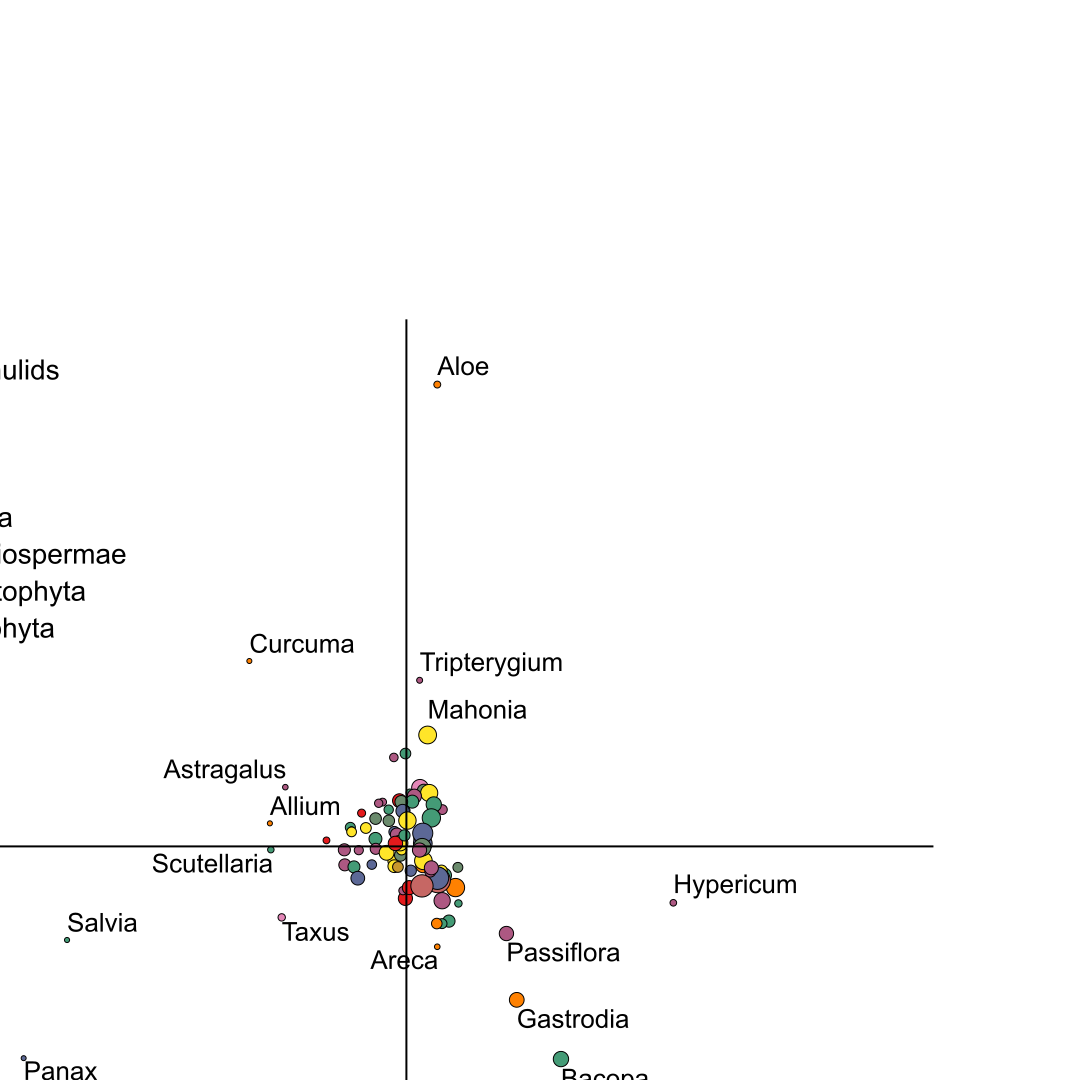
\includegraphics[width=0.9\linewidth]{textmining_diseases.png} \\ 
  \vskip 12pt
  \caption[m1]{
  \textbf{Отношения между лекарственными растениями и между группами хронических заболеваний}\itshape
  
  в левой части, размер кругов обозначает относительное количество публикаций с упоминанием лекарственного растения, а цветом обозначена группа, которой отнесено растение по его ботаническому описанию. 
  
  в правой части, размер кругов обозначает относительное количество публикаций, относящихся к заболеванию.
  
 } 
 \label{img:textmining_diseases}
\end{figure}

Часто в публикациях при описании лекарственного растения упоминают, в какой из традиций медицины принято было его использовать для лечения. И потому, в проведенной обработке текстов выделялись также географических термины, относящиеся к традициям медицины. Результаты, показанные на рис. \ref{img:relations_between_traditions}, основаны на разложении матрицы, составленной из связей между лекарственными растениями и традициями медицины. При обработке также были использованы термины "modern" и "official", чтобы охарактеризовать мето современной медицины среди традиций, выработанных при развитии цивилизации.

\begin{figure}[H]
  \centering
  \vskip 12pt
  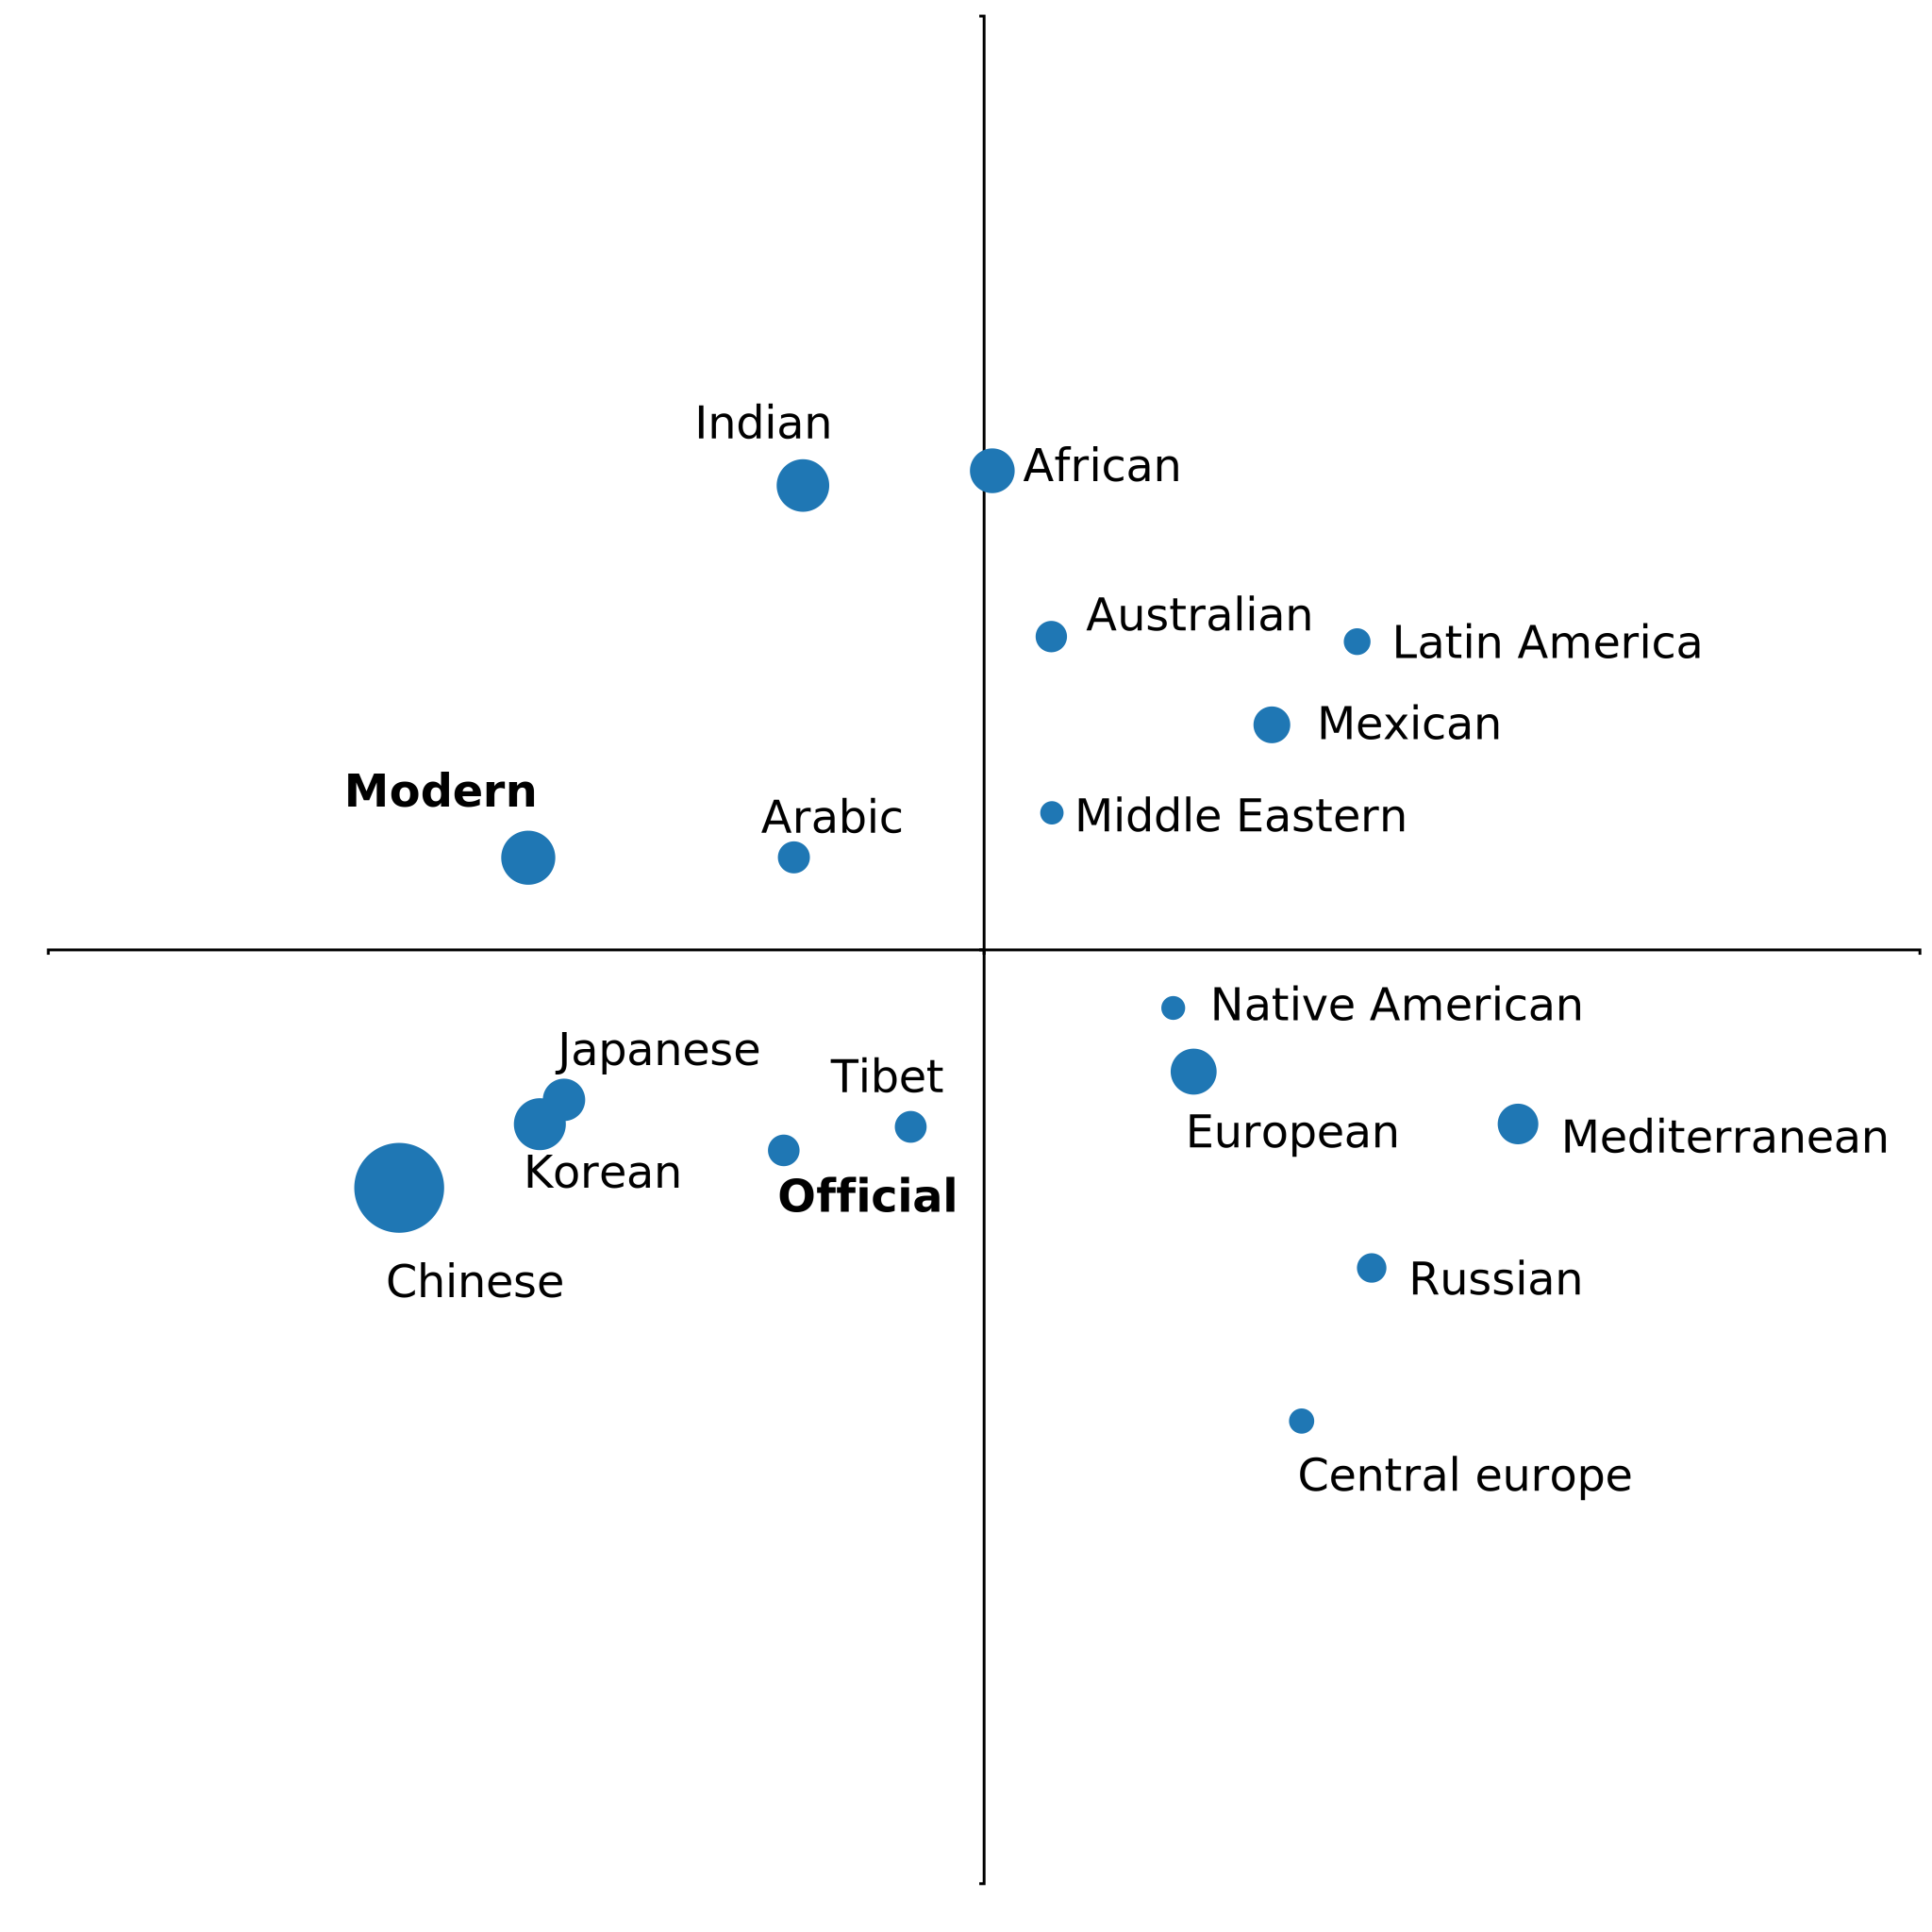
\includegraphics[width=0.5\linewidth]{relations_between_traditions.png} \\ 
  \vskip 12pt
  \caption[m1]{
  \textbf{Отношения между традициями медицины}\itshape
  
  размер кругов обозначает относительное количество публикаций, относящихся к традиции медицины.
} 
 \label{img:relations_between_traditions}
\end{figure}

В показанном способе расчета, традиционные "школы" медицины, с долей условности, разделены на культуры Востока, культуры Европы, и культуры народов Африки, Австралии и Америки. Подходы современной медицины, в этом представлении, подобны, в большей степени, культурам Востока. Но, говоря прямо, "переоцененные" научные идеи и термины, приводящие к накоплению систематических ошибок в современной науке, как это обсуждалось в разделах \ref{sect_expressionbiases}, \ref{sect_annotationbiases}, \ref{sect_medicine_comments}, следует сравнить с языческими богами, подобными языческим богам древних культур Востока. И потому обнаруженное сходство современной медицины с традициями Востока не следует считать неожиданным.

Другой подход к автоматической обработке текстов, описанный в \ref{sect_computationallinguistics}, где названию растения сопоставлялись названия генов, также был использован для оценки отношений между заболеваниями, по предполагаемому эффекту лекарственных растений. Для анализа были также использованы серии экспериментов RNA-Seq, где исследовалось различие в экспрессии генов в тканях, отобранных у пациентов, страдающих одним из заболеваний, и здоровых людей. Эффект лекарственного растения, оцененный, после обработки текстов, как направление регуляции некоторых генов, был обобщен до уровня, описывающего направление смещения полного профиля экспрессии генов. Это позволило сопоставить рассчитанные свойства растения со смещением профиля экспрессии, наблюдаемом в эксперименте, для каждого из заболеваний. Предварительная обработка серий экспериментов RNA-Seq, подобная описанной в разделе \ref{sect_expressionbiases}, была проведена, чтобы получить возможность использовать в основной серии расчетов обобщенные профили экспрессии.

\begin{figure}[H]
  \centering
  \vskip 12pt
  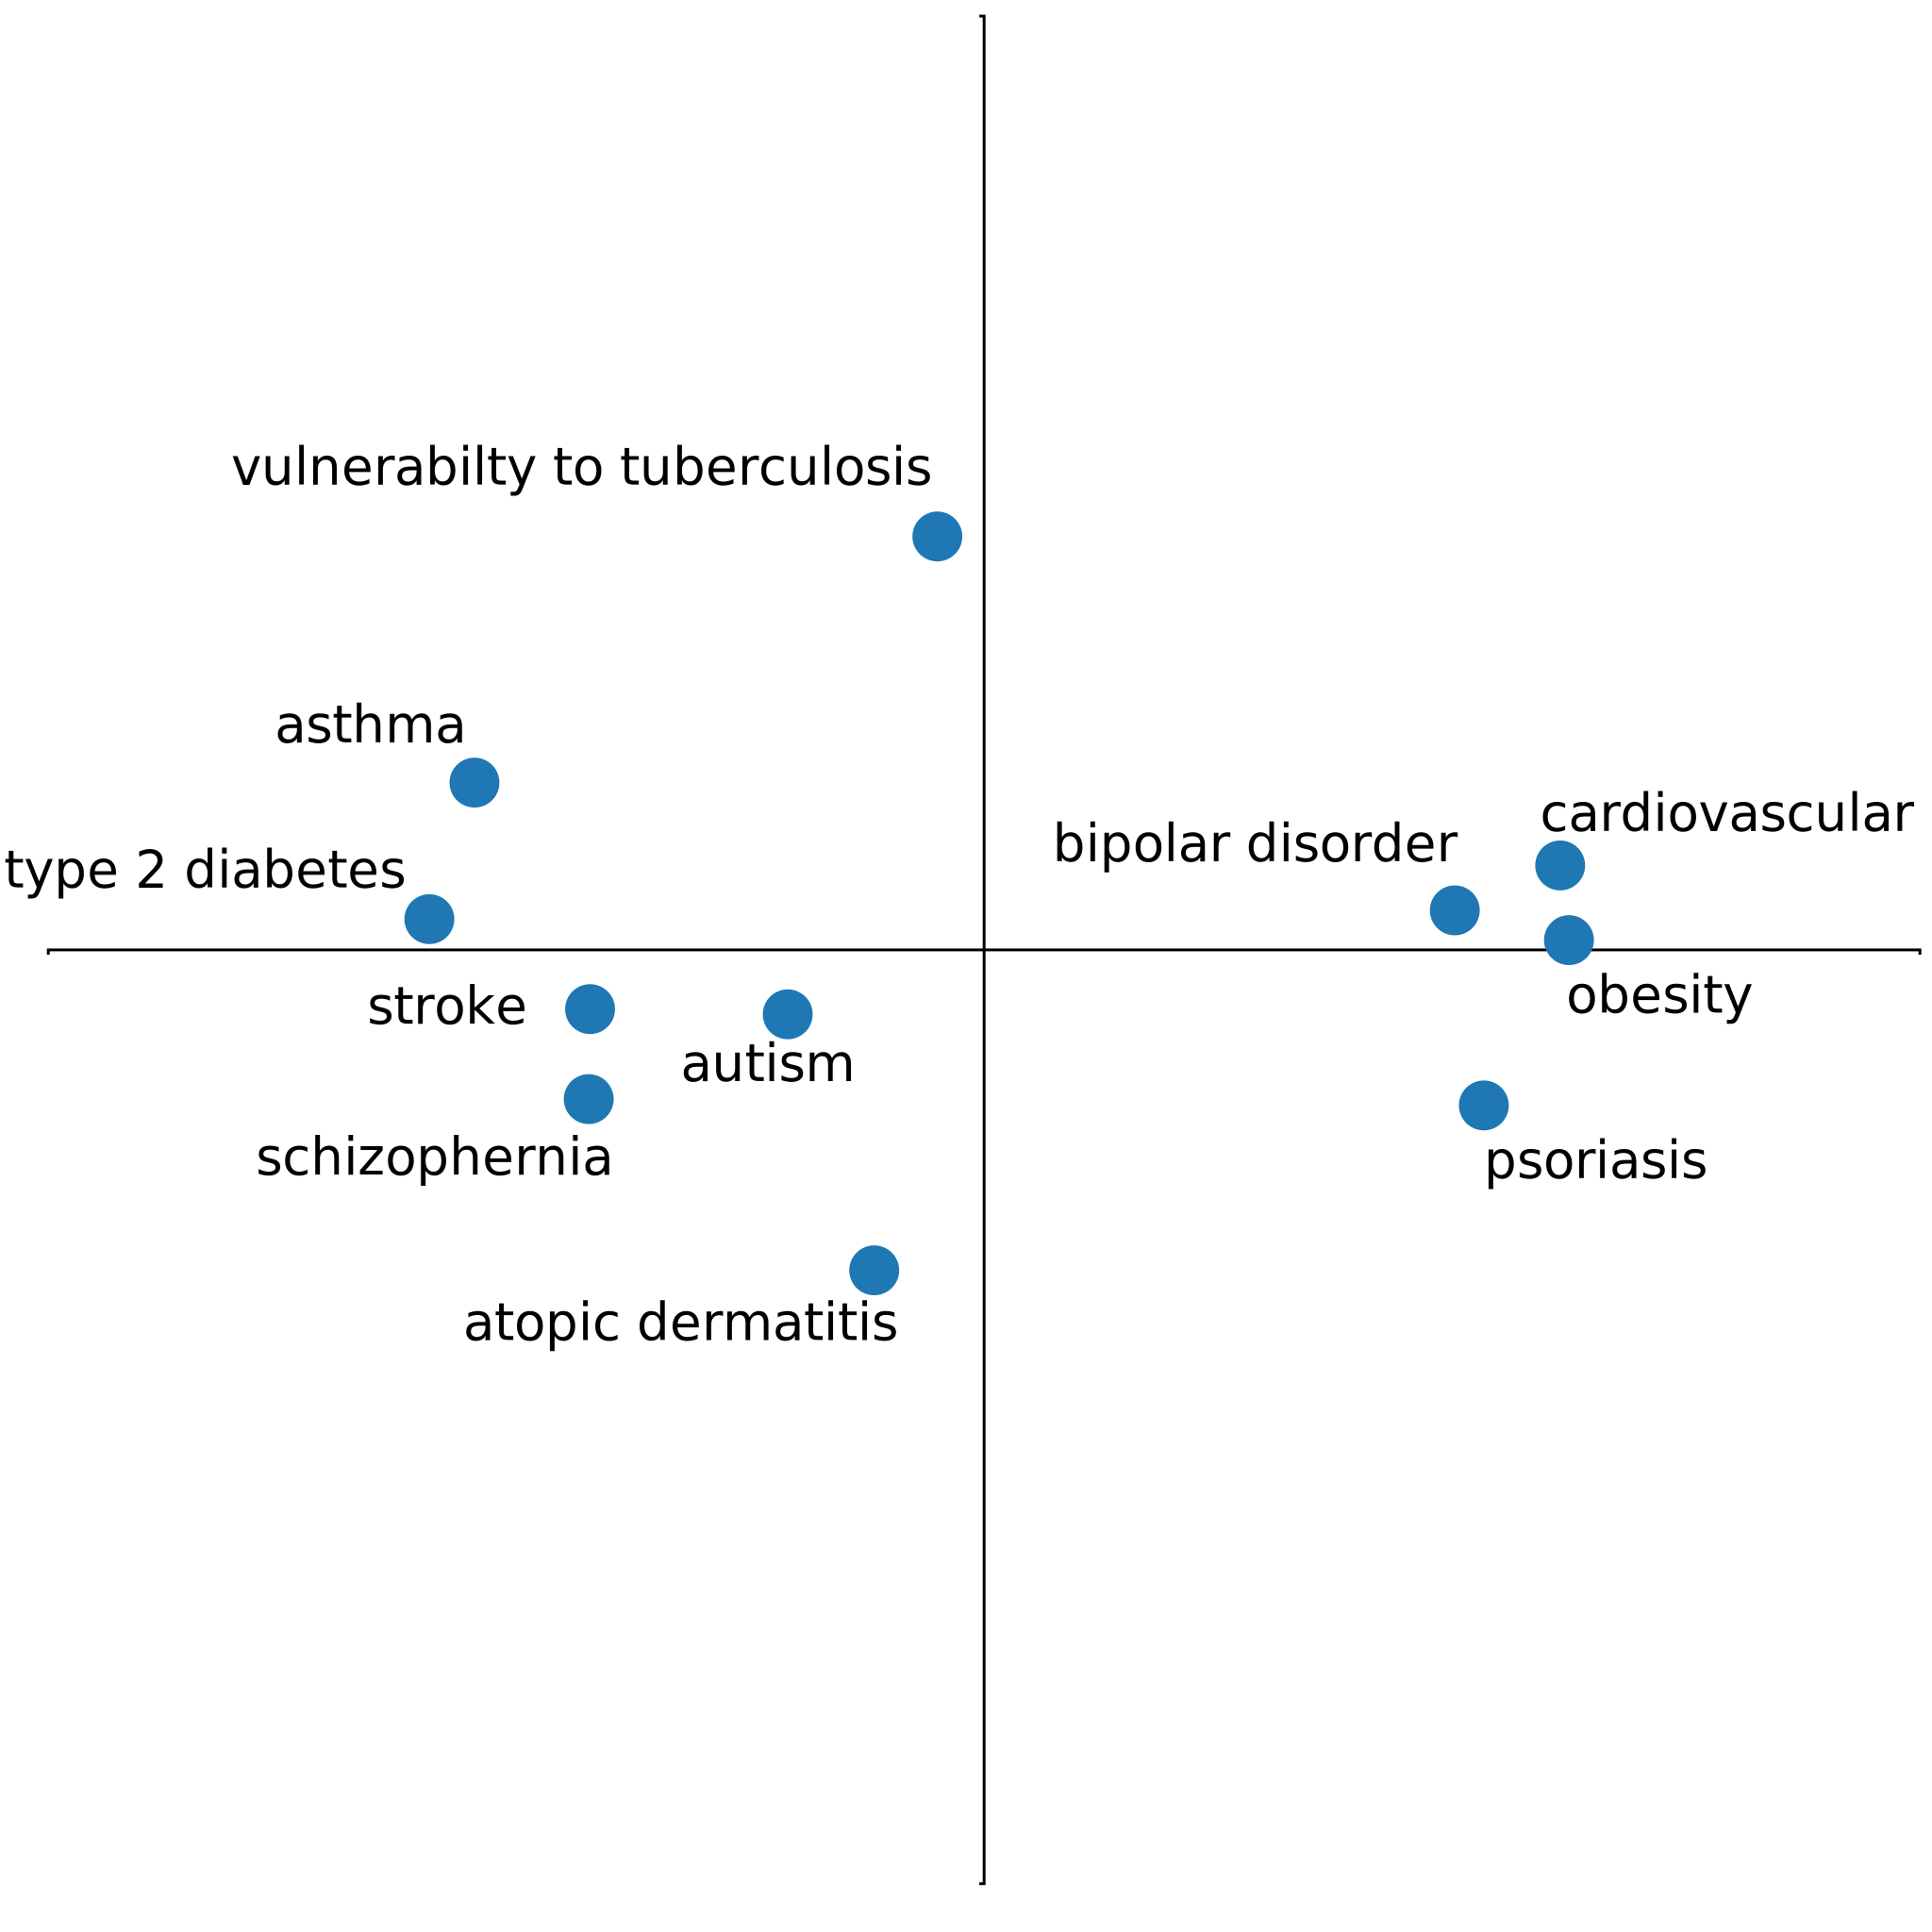
\includegraphics[width=0.5\linewidth]{herbs_rnaseq.png} \\ 
  \vskip 12pt
  \caption[m1]{
  \textbf{Отношения между хроническими заболеваниями, рассчитанные по данным экспериментов RNA-Seq}\itshape

 } 
 \label{img:herbs_rnaseq}
\end{figure}

Полученные при таком расчете соотношения между заболеваниями, показанные на рис. \ref{img:herbs_rnaseq}, не соответствуют соотношениям, полученным первым из подходов и показанные выше, на рис. \ref{img:textmining_diseases}. Но эти соотношения возможно согласовать, рассмотрев третью из главных компонент в представлении результатов PCA, оцененному при наиболее прямой обработке публикаций. При этом направление первой главной компоненты указывает, в основном, на систематические ошибки, вызванные смещениями акцентов в выборе тем исследования в обработанных публикациях. Полученное согласованное представление показано, с нескольких сторон, в заключительной части книги.


\section{Математические модели в биологии}

\subsection{Понятия из теории дифференциальных уравнений}

\noindent
\textbf{ \textit{Динамическая система} }

Система обыкновенных дифференциальных уравнений вида $\frac{dx}{dt} = F(x)$ может представлять модель некоторого объекта, для которого состояние описывается набором параметром $x = (x_i, i=1..N)$. Решение такой системы будет представлять эволюцию состояния объекта. В пространстве $N$ измерений, решение системы можно представить как траекторию изменения состояния объекта; такое пространство называется \textit{фазовым пространством}.

Описанная таким образом модель объекта может обозначаться термином \textit{динамическая система}. Возможно также рассмотреть динамические системы с дискретным шагом по времени, в отличии от представления с помощью дифференциальных уравнений, где ось времени является непрерывной.


\noindent
\textbf{ \textit{Устойчивость решения} }

Интуитивно, поведение динамической системы является устойчивым, если внесение малых отклонений в систему не приводят с течением времени к нарастающим отклонениям в траектории системы. Для системы дифференциальных уравнений, существуют более формальные определения устойчивости, в первую очередь - понятие "устойчивости по Ляпунову".


\noindent
\textbf{ \textit{Особые точки уравнений} }

Систему из двух обыкновенных дифференциальных уравнений, без явной зависимости от времени, можно записать в виде $\frac{dx}{dt} = F_x( x, y ), \frac{dy}{dt} = F_y( x, y )$. Решением этой системы будет пара функций $x_s(t), y_s(t)$, которую можно представить как кривую линию на плоскости, и можно интерпретировать как траекторию изменения системы. Скорость изменения системы при этом будет определять значениями функций $F_x, F_y$. Особыми точками в таком двумерном пространстве будут точки, в которых система неподвижна, то есть $F_x = F_y = 0$. В окрестности особых точек значения функций малы, и можно ограничится первым членом ряда Тейлора в разложении функций по обоим координатам. Упрощенные с помощью такого приближения уравнения несложно исследовать аналитически, и в результате возможно классифицировать возможные варианты поведения системы, разделив особые точки на три типа, как показано на рис. \ref{img:poincare}. В линейном приближении правая часть уравнений представляется как матрица 2x2, и тип особой точки определяется знаками собственных значений этой матрицы. Для вычисления собственных значений необходимо решить квадратное уравнение, и в некоторых случаях при вычислении решений необходимо использовать комплексные числа, поскольку значения решений будут выражаться через квадратный корень из отрицательного числа.


\begin{figure}[H]
  \centering
  \includegraphics[width=0.8\linewidth]{poincare.png} \\ 
  \caption[m1]{
  \textbf{Типы особых точек}\itshape
  
Фокус (слева) - собственные значения содержат мнимую часть; узел (в центре) - собственные значения одного знака; седло (справа) - собственные значения разных знаков.

\fontsize{10pt}{10pt}\selectfont
рисунок построен с помощью пакета matplotlib
} 
 \label{img:poincare}
\end{figure}

Для многих сложных многомерных дифференциальных уравнений, поиск положения и определение типа особых точек оказывается эффективным при аналитическом исследовании свойств уравнений.

\noindent
\textbf{ \textit{Предельный цикл} } - обобщение понятия особой точки, для описания решения уравнений, в которых траектория системы по мере эволюции системы приближается к циклическому движению, или в которых для любых начальных условиях система будет двигаться по циклической траектории. Обобщением понятия предельного цикла является понятие \textit{аттрактор}, когда устойчивой является траектория, не сводящаяся к циклической.

\noindent
\textbf{ \textit{Бифуркация} } - изменение характерных свойств динамической системы, при малом изменении параметров системы. Так, например, в системе $\frac{dx}{dt} = rx - x^3$, при $r<0$ устойчивым является решение $x=0$, а при $r>0$ - два решения $x=\pm\sqrt{r}$. В более широком смысле термин \textit{бифуркация} используют, например, для описания раздвоения русла реки, и т.п.

\noindent
\textbf{ \textit{Детерминированный хаос (динамический хаос)} } - поведение решения динамических систем, при котором внесение минимальных отклонений приводит к непредсказуемо большим последствиям при эволюции системы. В таком определении, понятие динамического хаоса обратно понятию устойчивости. 

\begin{figure}[H]
  \centering
   \begin{minipage}[ht]{0.49\linewidth}\centering
    \includegraphics[width=0.99\linewidth]{lorentz.png} \\ 
  \end{minipage}
  \hfill
  \begin{minipage}[ht]{0.49\linewidth}\centering
    \includegraphics[width=0.99\linewidth]{bifurcation.png} \\ 
  \end{minipage}
 %\includegraphics[width=0.5\linewidth]{lorentz.png} \\ 
 \caption[m1]{
 \textbf{Примеры систем с "детерминированным хаосом"}\itshape

Слева: Аттрактор Лоренца, решение системы дифференциальных уравнений, известной как "система Лоренца".

Справа: Карта бифуркаций в дискретной системе $x_{n+1}=r x_n ( 1- x_n ) $, известной как "логистическое отображение". Горизонтальная ось: величина параметра $r$. Вертикальная ось: точки, составляющие предельный цикл системы.

\fontsize{10pt}{10pt}\selectfont
рисунки по материалам проекта Wikipedia; credits: user PAR
} 
 \label{img:deterministic}
\end{figure}




\subsection{Обзор и частные случаи прикладных моделей} \label{sect_appliedmodels}

\noindent
\textbf{ \textit{Модель экспоненциального роста} } 

С помощью простейшего дифференциального уравнения $\frac{dx}{dt} = ax$ оказывается возможным описать, на некотором этапе, эволюцию многих систем разных масштабов, в том числе в приложениях биологии. Так, например, численность микроорганизмов при условии неограниченных ресурсов будет удваиваться с каждым циклом деления клеток. Решением записанного уравнения будет экспоненциальная зависимость от времени ($x(t)=\exp{at}$).


\noindent
\textbf{ \textit{Модель Лотка-Вольтерра ("хищник-жертва")} } 

Система из двух уравнений $\frac{dx}{dt}=(\alpha - \beta y)x; \frac{dy}{dt}=(\delta x - \gamma) y$ позволяет качественно описать отношения между биологическими видами ("хищником"и "жертвой"), при этом решением системы являются периодическая зависимость от времени, для численности популяций обоих видов. В фазовом пространстве, решения уравнения Лотки-Вольтерра представляются как циклические кривые, и особая точка этого уравнения может быть классифицирована как фокус (рис. \ref{img:poincare}) 

\noindent
\textbf{ \textit{Обобщенная модель сосуществования двух видов} } 

Для описания возможных отношений между двумя видами в математической экологии используются дифференциальные уравнения с двумя переменными, обобщающие модель Лотки-Волтерра. При этом, классификацию отношений между видами можно свести к классификации особых точек дифференциальных уравнений. При этом используют следующие термины: "+/+" (узел) - \textit{симбиоз} или \textit{мутуализм}; "+/-" (фокус) = \textit{хищник - жертва} или \textit{паразит  - хозяин}; "-/-" (седло) - \textit{конкуренция}.

\noindent
\textbf{ \textit{Модель инфекционного заболевания} }

В иммунном ответе организма при инфекционном заболевании участвуют многие типы клеток, и потому модели, описывающие развитие инфекционного заболевания в организме, не сводятся к простейшей модели отношений между паразитом и хозяином. Для некоторых вариантов расширенных моделей, в которых учитывается несколько стадий иммунного ответа, возможно получить решения, соответствующие острому и хроническому течению заболевания. С использованием таких моделей возможно качественно исследовать эффект так называемого "лечения через обострение", для перевода хронического заболевания в острое, с последующим полным выздоровлением. Однако степень сложности в организации иммунной системы, как правило, не позволяет довести соответствие моделей до уровня количественного описания заболевания.

\silentheader

\begin{figure}[H]
  \centering
   \begin{minipage}[ht]{0.49\linewidth}\centering
    \includegraphics[width=0.99\linewidth]{lotkavolterra.png} \\ 
  \end{minipage}
  \hfill
  \begin{minipage}[ht]{0.49\linewidth}\centering
    \includegraphics[width=0.9\linewidth]{trophic.png} \\ 
  \end{minipage}
 %\includegraphics[width=0.5\linewidth]{lorentz.png} \\ 
 \caption[m1]{
 \textbf{Иллюстрации к некоторым темам математической экологии}\itshape

Слева: Фазовая диаграмма решений уравнения Лотка-Вольтерра. Горизонтальная ось - условное количество "жертв"; вертикальная ось - условное количество "хищников". Траектории с разными начальными условиями показаны разным цветом.

Справа: Сводная схема связей между видами цветковых растений и видами птиц, которые их опыляют, по материалам полевых исследований на островах Галапагосского архипелага. 

\fontsize{10pt}{10pt}\selectfont
Рисунок слева: по материалам проекта Wikipedia; credits: user Brice2000. Рисунок справа: работа \parencite{Traveset_2015}.
} 
 \label{img:ecology}
\end{figure}

Колебательные явления, которые возможно описать лишь с помощью системы нелинейных уравнениями, можно наблюдать даже в неорганической химии (так называемая "реакция Белоусова-Жаботинского"). И потому уместно применение методов из теории динамических систем для описания биохимических процессов в клетке. Но описание некоторых явлений в многоклеточных организмах возможно только с использованием моделей динамических систем. Так, например, с использованием понятия бифуркации (так называемой "бифуркации Тьюринга") можно качественно описать появление полос на кожу у зебры, пятен у леопарда, и пр. Понятие бифуркации, в более широкой перспективе, описывает и само явление морфогенеза, когда соседние и однотипные клетки при делении дифференцируются в ткани различных органов.

Помимо упомянутой модели ответа иммунной системы на инфекционное заболевание, составлены модели для описания образования единого  ритма в синусном узле сердца, в результате согласования активности клеток, называемых пэйсмэйкерами (pacemaker), а также модели распространения электрического импульса по тканям сердца. С помощью модели тока ионов натрия и калия в нейроне возможно описать распространение так называемого "потенциала действия" по протяженному аксону. Сложность устройства нервной системы не позволяет с достаточной адекватностью описать принципы, лежащие в основе мышления, однако исследования различных моделей сетей нейронов интенсивно развиваются, как будет подробно описано ниже.

Наконец, вся теория динамических систем, по своему происхождению и по степени применимости, тесно связана с описанием структуры и динамики экосистем. Для модельного описания отношений между видами в экосистеме, используют понятие \textit{трофические сети}. При построении такой сети, связь между двумя биологическими видами устанавливается в терминах классификации отношений между видами, описанной выше. Также, на основании свойств графа трофических отношений, среди биологических видов выделяют так называемых "дженералистов" (\textit{generalist}) - условно, "всеядные" виды, и "специалистов" (\textit{specialist}), виды, адаптированные к определенному типу питания. 

Динамика численности популяций при таком описании может быть в некоторых случаях сведена к отношениям между парами взаимодействующих видов, как это описано выше. В других случаях, в решениях уравнений проявляется "динамический хаос", как свидетельство ограниченности попыток описания экосистем с использование подобного класса методов. Также, существование эффекта, для обозначения которого используется понятие \textit{видообразование}, неявно ограничивает применимость описанных методов.

\subsection{Нейробиология и модели сетей нейронов}

Исследования, проводимые в области нейробиологии, науке изучающей работу нервной системы, сопоставимы по объему и интенсивности с исследованиями во всей молекулярной биологии, включая методы и подходы биоинформатики. И потому обсуждение методов и результатов, полученных в нейробиологии, выходит за рамки настоящего курса. Но модели сетей нейронов, построенные на основании сведений из нейробиологии, являются нетривиальными примерами моделей биологических систем. Обзор этих моделей, а также смежных понятий нейробиологии, приведен ниже. При построении моделей нейронных сетей вводится последовательный ряд упрощений и приближений; не все эти упрощения и не все исключения из правил оговариваются явно.


%, хотя эти модели в полной мере и не отражают степень сложности в устройстве нейрвной системы, и не позволят объяснить принципы, лежащие в основе мышления.

\begin{figure}[H]
  \centering
  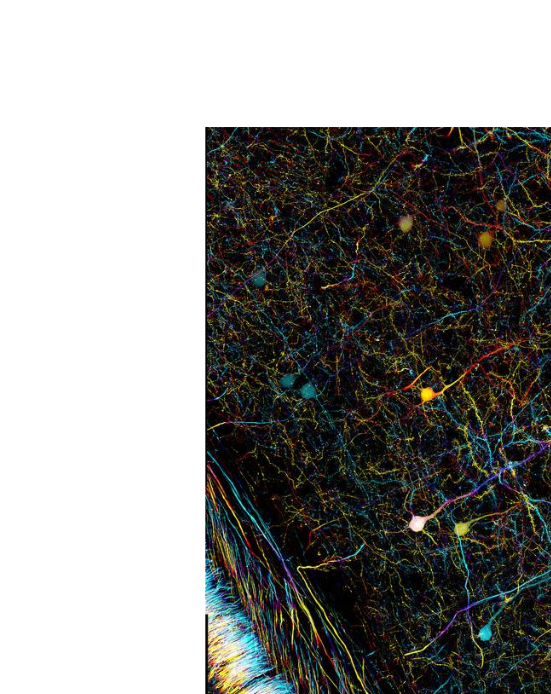
\includegraphics[width=0.99\linewidth]{neural.png} \\ 
  \caption[m1]{
  \textbf{Принципы устройства сети нейронов}\itshape
  
Слева: кора головного мозга мыши, конфокальная лазерная сканирующая микроскопия.

Справа: схема устройства нейрона и синаптической щели. A - аксон, B - дендрит, C - нейромедиатор.
  
\fontsize{10pt}{10pt}\selectfont
Credits: ZEISS Microscopy;  Mouagip, Dake, Quasar Jarosz (Wikipedia).
} 
 \label{img:neural}
\end{figure}

Крупные и разветвленные клетки головного мозга, называемые \textit{нейронами}, являются основой для происходящих в организме  процессов хранения и переработки информации. Особенностью нейронов является возможность находиться в состоянии "возбуждения", что выражается в изменении электрического потенциала цитоплазмы по отношению к внешней среде. Разность потенциалов при этом  поддерживается за счет переноса ионов натрия, калия и кальция через каналы в мембране нейрона. Состояние возбуждения может передаваться другим нейронам, через соединения между разветвленными частями двух нейронов, называемые \textit{синапсами}.

Накопление возбуждения, передаваемого соседними нейронами через ответвления клетки, называемые \textit{дендритами}, приводит к переходу в возбужденное состояние, и затем импульс возбуждения передается по ответвлению, называемому \textit{аксоном}, следующим нейронам. При этом синапсы, через которые передается возбуждение, могут различаться по типам нейромедиатора и по интенсивности передаваемого сигнала. Для некоторых нейромедиаторов, сигнал, передаваемый через синапс, может приводить к торможению клетки, принимающей сигнал, а не к увеличению ее возбуждения.

Для описания разных категорий и свойств нейронных сетей предложено достаточно много подходов. Некоторые из моделей описывают развитие нейронной сети, выражающееся в изменении коэффициентов передачи сигнала в синапсах (так называемых \textit{весов} связей). Другие модели описывают изменение интенсивности возбуждения клеток, при допущении, что веса связей не меняются при моделировании. 

\begin{table}[htbp]
\caption{Подходы к моделированию нейронных сетей}\label{tab:ann_models}
\begin{tabular}{|c|c|c|}
\hline
\makecell{Наименование}&\makecell{\rotatebox{90}{наличие циклов}}&\thead{Комментарий}\\
\hline
{\small Обучение Хебба}& - &{\itshape \small принцип ассоциативной памяти}\\
\hline
{\small "Перцептрон"}& нет &{\itshape \small модель распознавания образов при обучении "по образцу"}\\
\hline
{\small Обратное распространение ошибки}& нет &{\itshape \small алгоритм коррекции весов связей для сетей без циклов}\\
\hline
{\small Сеть Кохонена}& - &\makecell{{\itshape \small используется для задач разделения на классы,}\\{\itshape \small без задания образцов}}\\
\hline
{\small Сеть Хопфилда}& есть &{\itshape \small модель сети с циклами, как динамическая система}\\
\hline
{\small "Победитель забирает все"}& есть &\makecell{{\itshape \small частный случай сети Хопфилда,}\\{\itshape \small каждый нейрон связан с остальными}\\{\itshape \small тормозящими связями.}}\\
\hline
{\small Ассоциативная сеть}& есть &{\itshape \small модель сети с циклами, как ассоциативная память}\\
\hline
{\small Глубинное обучение}& нет &{\itshape \small уточненные методы настройки сети без циклов}\\
\hline
\end{tabular}
\end{table}

По топологи нейронной сети можно разделить модели, в которых граф сети не содержит циклов, и модели, где в графе допускаются циклы (рис. \ref{img:neural_artificial}). В большей части моделей, для расчета возбуждения нейрона сигналы из входных нейронов суммируются с учетом весов связей. Но вид функции, связывающей итоговый входной сигнал и уровень возбуждения нейрона, зависит от выбора модели.

Модели сетей без циклов (рис. \ref{img:neural_artificial}, слева) были предложены одними из первых и разработаны в наибольшей степени. Эти модели нашли приложения в решении задач классификации, и в уточненном виде, в технологиях, которые обозначаются термином \textit{deep learning} ("глубинное обучение"). Настройка топологии, весов связей и формы преобразования входного сигнала в таких сетях производятся на так называемой \textit{стадии обучения}, за которой следует стадия использования сети для решения задач классификации.

\begin{figure}[H]
  \centering
  \includegraphics[width=0.65\linewidth]{neural_artificial.png} \\ 
  \caption[m1]{
  \textbf{Принципы построения моделей сетей нейронов}\itshape
  
Слева - сети без циклов; справа - сети с циклами.

Вверху - структура сети, внизу - возбуждение в сети. Возбужденные нейроны помечены темно-синим. Тормозные синапсы обозначены кружками.
} 
 \label{img:neural_artificial}
\end{figure}


При моделировании сетей с циклами (рис. \ref{img:neural_artificial}, справа), решением является устойчивое состояние сети, один из аттракторов, к которому сходится фазовое состояние системы, в зависимости от уровней возбуждения клеток в начале моделирования. Возможно использование такой сети (\textit{"сети Хопфилда"}) для решения некоторых комбинаторно сложных задач. Веса связей при таком подходе определяются условиями задачи, а состояние сети, полученное при моделировании, следует преобразовать в оптимальный выбор варианта при переборе.

\begin{figure}[H]
  \centering
   \begin{minipage}[ht]{0.49\linewidth}\centering
    \includegraphics[width=0.3\linewidth]{hopfield_dog_noised.png} \\ 
  \end{minipage}
  \hfill
  \begin{minipage}[ht]{0.49\linewidth}\centering
    \includegraphics[width=0.3\linewidth]{hopfield_dog.png} \\ 
  \end{minipage}
 %\includegraphics[width=0.5\linewidth]{lorentz.png} \\ 
 \caption[m1]{
 \textbf{Пример восстановления повреждённого изображения с использованием ассоциативной сети}\itshape

Слева: искаженный образ; справа: эталон.

\fontsize{10pt}{10pt}\selectfont
По материалам проекта Wikipedia.
} 
 \label{img:hopfield_dog}
\end{figure}

Более практичная и простая для восприятия модель приложения сетей с циклами - это возможность выбора одного из возможных вариантов состояния, заложенных на стадии обучения. Так, например, сопоставив клетки сети с точками изображения, можно использовать модель для восстановления искаженного изображения (рис. \ref{img:hopfield_dog}). Сеть может быть обучена для выбора одного из нескольких возможных изображений. Для выбора весов связей на стадии обучения возможно использовать так называемое \textit{правило Хебба} (Hebb's rule). В общем случае, веса связей устанавливаются на основании ассоциаций между клетками в изображениях, используемых для обучения. Ограничения применения сетей с циклами в такой постановке связаны со слишком малым (порядка $N/\log (N)$, где $N$ - размер сети) количеством шаблонов, среди которых возможно выбрать решение. 


\subsection{Модель сети нейронов с двумя типами возбуждения} \label{sect_neuro_layers}


Простейшей моделью, состоящей из двух нейронов, является модель \textit{"winner takes all" ("победитель забирает все")} (рис. \ref{img:neural_dyn}, слева), частный случай сети Хопфилда. Эта модель, где два нейрона соединены между собой подавляющими связями, иллюстрирует, как мозг принимает решения, не попадая в ситуацию "Буриданова осла". Система имеет два устойчивых состояния, выбор между которыми может происходить до какой-то степени случайно, когда в начале оба нейрона не возбуждены. Когда один из нейронов становится возбужденным, в рамках модели система продолжает оставаться в устойчивом состоянии; вопрос о возврате в невозбужденное состояние можно поставить только в более широком контексте.

\begin{figure}[H]
  \centering
  \includegraphics[width=0.75\linewidth]{neural_dyn.png} \\ 
  \caption[m1]{
  \textbf{Модель «Winner takes all»}\itshape

Возбужденные нейроны помечены темно-синим. Связи показаны стрелками; неактивные связи показаны пунктиром. Справа показано возможное расширение модели за счет учета слабых уровней возбуждения (светло-синий).
} 
 \label{img:neural_dyn}
\end{figure}


Более внимательный анализ существующих в мозге синапсов позволяет уточнить, что в большинстве синапсов медиатором служат глутамат и аспартат.
Но в некоторых синапсах в ЦНС используется для передачи возбуждения медиатор ацетилхолин, основной медиатор в периферической нервной системе. При этом механизмы, через которые в ЦНС возбуждение передается через глутаматовые и ацетилхолиновые синапсы, принципиально отличаются тем, что: 
\begin{itemize}
\vspace*{-10pt}
\item возбуждение клетки через рецепторы ацетилхолина приводит к высвобождению ионов кальция и интенсивному поглощению энергии возбужденной клеткой, 
\vspace*{-10pt}
\item возбуждение клетки через рецепторы глутамата регулирует в основном обмен ионов натрия и калия и не приводит к интенсивному поглощению энергии.
\end{itemize}
%\vspace*{-10pt}

В предположении о двух типах возбуждающих синапсов, в модель "winner takes all" можно внести дополнение (рис. \ref{img:neural_dyn}, справа). Если предположить, что возбуждение в этой модели передается ацетилхолиновыми связями, то предварительное малое возбуждение клетки через дополнительные рецепторы глутамата может обусловить выбор устойчивого состояния при появлении необходимости сделать такой выбор.

\begin{figure}[H]
  \centering
  \includegraphics[width=0.7\linewidth]{neural_dyn_layers.png} \\ 
  \caption[m1]{
  \textbf{Модель многослойной сети с двумя направлениями передачи информации}\itshape
  
Слой примерно соответствует ассоциативной сети. Шаги 1, 2 показывают этапы передачи информации. Возбужденные нейроны помечены темно-синим. Слабо возбужденные нейроны показаны светло-синим. Два типа связей показаны стрелками двух типов.
} 
 \label{img:neural_dyn_layers}
\end{figure}

Эту модель можно обобщить и предположить, что в мозге существует два направления распространения информации (рис. \ref{img:neural_dyn_layers}). Первое направление служит для регулировки и подстройки и передается через рецепторы глутамата; тогда как, информация второго рода приводит в итоге к возбуждению мышц и передается через рецепторы ацетилхолина. Разделение сети на слои, схематично показанное на рис. \ref{img:neural_dyn_layers}, совместимо с предположением о двух направлениях передачи информации. Связи внутри каждого слоя при этом предполагаются тормозящими, как и между парой нейронов в модели "winner takes all". Допущение об отделении этого, третьего, типа связей, сигнал от которых приводит к безусловному подавлению активности клетки, также согласуется с данными нейробиологии. Медиатором в большей части тормозных синапсах является \textit{гамма-аминомасляная кислота} (ГАМК), и при торможении через рецепторы ГАМК наблюдают эффект "шунтирования" (\textit{shunting inhibition}), безусловного подавления остальных потупающих в клетку сигналов. 

Разделение сети нейронов на слои в модели сети, хотя это и условное схематичное представление нервной системы, соответстует возможности разделения всего объема знаний об окружающем мире, сохраняющемся в ЦНС, на относительно независимые фрагменты. Язык человека отражает способ его мышления, и  первичными фрагментами при передачи знания в языке являются слова, примерно соответствующие четко отделяемым объектам и устойчивым понятиям окружающего мира, так что значение каждого слова понятно как говорящему, так и слушающему. Каждый из объектов может быть устроен сколь угодно сложно, но, представив возможные и практически значимые состояния объекта как перечисляемое множество, модель такого объекта возможно составить из ограниченного числа нейронов, объединенных в общий слой через тормозящие связи.

В простейшем примере слоя, сети "winner takes all", количество нейронов определяет возможные состояния, а активность одного из нейронов в слое - выбор из возможных состояний. В сети "winner takes all" все нейроны связаны между собой тормозящими связями, но, убрав из подобной сети некоторые из связей, количество возможных состояний следует скорректировать, и в некоторых из состояний могут быть активны сразу несколько нейронов. При "подстройке" ("обучении") сети, переход типа связи от тормозящей к нейтральной, и обратно, позволяет "подогнать" систему связей в слое к объекту, который моделирует этот слой. Слой в описываемой сети следует рассматривать в контексте взаимодействия с другими слоями, и описанный процесс обучения, открывая возможность быть активными сразу нескольким нейронам в слое, позволяет настроить, среди свойств объекта, варианты его взаимодействия с другими объектами. С этим способом настройки модельной сети можно связать описанный в нейробиологии эффект переключения направления регуляции в рецепторах ГАМК при развитии мозга.

Разделение сети на слои в предложенной модели позволяет прояснить, как мозг способен принимать решения настолько быстро, при огромном объеме сохраняемых там знаний. А именно, в устройстве модели можно заметить сходство с моделью сворачивания белка (раздел \ref{protein_folding}), где черты принципа "разделяй и властвуй" совмещены с разделением задачи на согласованные части. В алгоритмах, относящихся к "динамическому программированию", где также проводятся расчеты по подобной схеме, с необходимостью вводятся два этапа, подобные двум направлениям передачи информации в описанной модели.

При моделировании некоторой системы по законам физики, возможность рассчитать, хотя бы приближенно, поведение системы, увязана со степенью независимости частей, составляющих эту систему. Подобно этому, при настройке разделения сети на слои, в описываемой модели, переключение тормозящей связи до уровня нейтральной может отражать факт независимости отдельных объектов, и существенно повышать эффективность работы сети.  

Парадоксальное отличие человека, и его поведения, от компьютерной системы, в том что, в отличии от человека, алгоритм для компьютера составляет разработчик, находящийся вне этой системы. Для животных, подобных человеку по анатомии и по устройству нервной системы, можно также примерно указать цели, определяющие поведение и необходимые для выживания особи и вида в целом. Поток информации, поступающий в мозг от органов чувств, подобен входным данным в компьютерной программе. Но цели поведения, как, например, потребность в пище, и даже потребность в пище определенного рода, можно рассматривать как поток информации другого рода, чем сигналы, посылаемые органами чувств.

\begin{figure}[H]
  \centering
  \vskip 12pt
  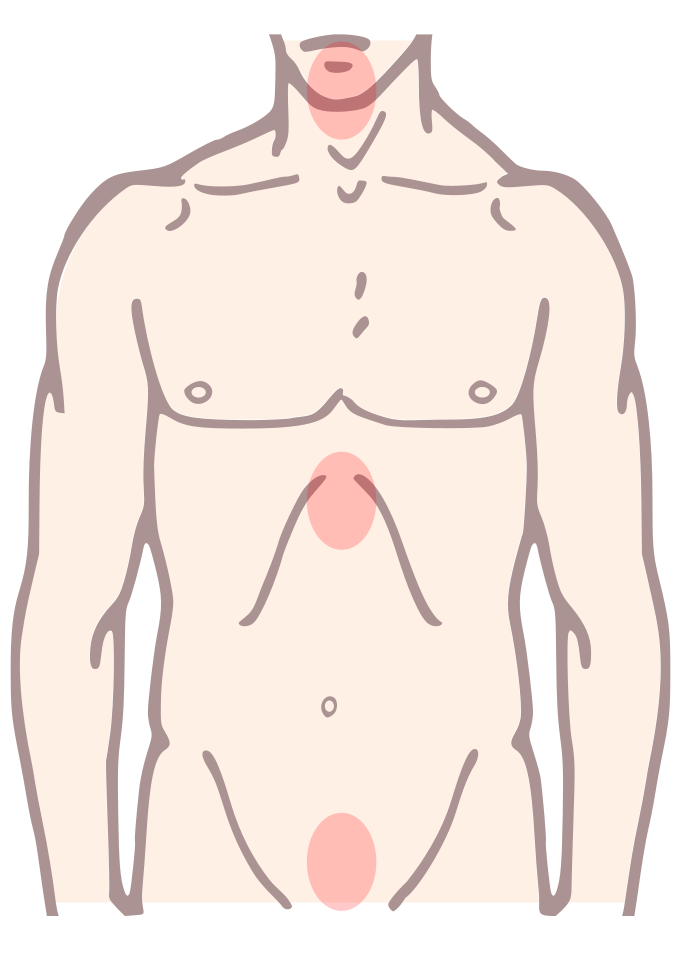
\includegraphics[width=0.4\linewidth]{neural_plexuses.png} \\ 
  \vskip 12pt
  \caption[m1]{
  \textbf{Головной мозг и некоторые из "сплетений" в периферической нервное системе}\itshape
  
  \fontsize{10pt}{10pt}\selectfont
  credits: NASA
} 
 \label{img:neural_plexuses}
\end{figure}

Модель, предполагающая два направления распространения информации, позволяет увязать меняющиеся и определяемые вне мозга цели поведения со "слабыми" сигналами, передающимися через рецепторы глутамата. Этот род информации определят выбор из возможных альтернатив, когда от органов чувств приходит "сильный" сигнал, требующий немедленной реакции и распространяющийся по второму направлению, вплоть до возбуждения мышц.

Как все хорошо знают, поведение человека в полной мере не определяется его потребностями в насыщении и продолжении рода. Но, так же как цели поведения животного определяются вне мозга, цели и желания человека, любого рода, не следует искать внутри мозга. И потому, несмотря на то, что современные экспериментальные методы позволяют примерно локализовать в мозге зоны, относящиеся к владению языком или к восприятию языка искусства, категории информации такого рода не относятся непосредственно к целям поведения человека. Информация об их локализации и динамическом изменении не имеет смысла, хотя бы даже при намерениях прогнозировать и управлять поведением человека. 

Прицельное воздействие на мозг, при примерном знании его устройства, может нанести травму психике. Эта травма может выражаться введением в состояние гипноза, но вопрос свободы воли человека при этом все же не имеет отношения к вопросу о его психическом здоровье. Регуляция дыхания и сердцебиения, необходимость в воздухе и циркуляции крови - наиболее глубокие и неотъемлемые из потребностей живого существа. И материя, в которой воплощена свобода воли человека, может быть увязана только с механизмами регуляции этих глубинных процессов. Так или иначе, но подлинные мотивы, руководящие человеческим разумом, следует искать за пределами человеческого разума.

%Эти части тела тоже могут быть поражены болезнями, самыми опасными из болезней, но все же сказано "{\emfont \itshape \small Возьмите Иго мое на себя и научитесь от Меня, ибо Я кроток и смирен сердцем, и найдете покой душам вашим}".

%Модель с двумя направлениями распространения информации известна в математике как концепция динамического программирования. В рамках этой концепции построены решения сложных комбинаторных задач за полиномиальное время, среди них – задача парного выравнивания последовательностей. Возможно, высокая эффективность и скорость работы мозга может быть объяснена через параллели с этой математической концепцией.

\subsection{Элементы теории фракталов} \label{sect_fractalmodels}

Термин \textit{фрактал} был введен в 1960-1970 годы в серии работ Б. Мандельброта; в его статье «Какова длина побережья Британии» он применил понятие дробной размерности для описания так называемого «парадокса береговой линии», замеченного ранее  Л.Ф. Ричардсоном. Парадокс береговой линии, который демонстрирует затруднения при измерении длины береговой линии, проиллюстрирован на рис. \ref{img:fractal_coast}. Определения размерности Хаусдорфа или размерности Минковского, введенные в математику в начале XX века, позволяют рассчитать дробную (нецелую) размерность для некоторых специфических объектов геометрии. И подобные методы могут быть применены к описанию объектов, возникающих как явления природы. Цитируя Б. Мандельброта: «Облака - не сферы, горы - не конусы, береговые линии - не окружности, древесная кора не гладкая, и молния - далеко  не прямая...» 

\begin{figure}[H]
  \centering
  \includegraphics[width=0.5\linewidth]{fractal_coast.png} \\ 
  \caption[m1]{
  \textbf{Побережье Британии, измеренное в нескольких масштабах}\itshape

слева: единица длины - 200 км, длина побережья - около 2400 км; справа: единица длины - 50 км, длина - 3400 км

\fontsize{10pt}{10pt}\selectfont
Credits: Avsa, Wapcaplet, Acadac (Wikipedia)
} 
 \label{img:fractal_coast}
\end{figure}


Объекты, которые можно описать как фракталы, возникают при различных обстоятельствах и их появление нельзя свести к наличию единого механизма развития. Свойства фрактальной структуры могут быть обнаружены в любом объекте, выделенном в окружающем мире, если в распределении его геометрических свойств, построенном в логарифмических координатах, обнаруживается линейная зависимость, как в примере, показанном на рис. \ref{img:fractal_strassbourgh}. 

\begin{figure}[H]
  \centering
  \includegraphics[width=0.8\linewidth]{fractal_strassbourgh.png} \\ 
  \caption[m1]{
  \textbf{Фрактальной структура дорожной сети в Страсбурге}\itshape

\fontsize{10pt}{10pt}\selectfont
по материалам \parencite{Wang_2017}
} 
 \label{img:fractal_strassbourgh}
\end{figure}


В линейных координатах, эта зависимость будет выражаться так называемым \textit{степенным законом} (power law), $ y = A^D $; значение $D$, с отрицательным знаком, будет значением фрактальной размерности. Фрактальное представление сложных геометрических объектов позволяет охарактеризовать структуры с помощью одного параметра $D$, значения фрактальной размерности. Точное значение фрактальной размерности может быть разным для одного и того же объекта, в зависимости от методов, используемых для расчета размерности. Но, в рамках любого метода оценки, величина $D$ может иметь точность, достаточную для использования этого значения при сравнении нескольких сопоставимых объектов, обеспечивая статистическую значимость выводов, полученных на основе такого сравнения.

%(Елинек и Фернандес, 1998). Альтернативная интерпретация заключается в том, что методы теория фракталов обеспечивает эффективный способ оценки количество независимых переменных в многомерном данные (Карбаускайте и Дземуда, 2016). 

Зависимость в форме степенного закона может быть замечена не только в свойствах геометрических объектов, но и в распределениях, относящимся к другим категориям и предметным областям. Распределение вероятностей, известное как \textit{закон Ципфа}, описывающее частоту встречаемости слов в текстах на естественных языках, также является частным случаем степенного закона. В законе Ципфа,  частота, с которой слово встречается в тексте, обратно пропорциональна его порядковому номеру в списке слов, отсортированном по количеству случаев использования каждого слова. Другим примером эмпирически обнаруженного степенного закона, относящимся к экономике, является \textit{распределение Парето}. Это распределение было получено как обобщение наблюдения Вилфредо Парето о том, что 20\% населения Италии владеет 80\% ее земель. В общем случае, распределение Парето используют в экономике и социологии как модель распределения доходов или финансовых активов любого рода.

В некоторых случаях, когда степенного закона недостаточно, чтобы объяснить распределение полученные путем применения фрактальных подходов к изучаемой системе, используется так называемое \textit{мультифрактальное} представление, где величина фрактальной размерности обобщается как  непрерывный ряд показателей степени в степенном законе. Более простое по форме обобщение степенного закона используется в так называемой \textit{эконофизике} (econophysics), для описания распределения доходов и активов в социологии.

Сам Б. Мандельброт указывал на принципиальное различие между вероятностными распределениями, описываемыми степенным законом, и вероятностными распределениями на основе распределения Больцмана, используемыми в статистической физике. Методы статистической физики, на его взгляд, приводят к значительно более предсказуемым результатам, по сравнению с фрактальными распределениями. Однако в эконофизике, с использованием нескольких достаточно простых моделей перераспределения доходов, было показано, что оба типа распределений могут быть совмещены в рамках единого подхода (рис. \ref{img:fractal_boltzmann}).

\begin{figure}[H]
  \centering
  \includegraphics[width=0.7\linewidth]{fractal_boltzmann.png} \\ 
  \caption[m1]{
  \textbf{Некоторые примеры описания данных с использованием совместно экспоненциального и степенного распределений вероятностей}\itshape

Слева: распределение вероятностей описывающее доходы населения США, по результатам обработки налоговых деклараций.
Теоретическое распределение показано линями, данные федеральной резервной системы США показаны символами. Функции распределения показаны в логарифмическом масштабе, после перенормирования. Данные за разные годы сдвинуты по вертикали. 

Справа: распределения относительной численности филотипов бактерий в микробиомах донных осадков, показанные в логарифмическом масштабе.

\fontsize{10pt}{10pt}\selectfont
использованы материалы \parencite{Banerjee_2010} и работы авторов курса.
} 
 \label{img:fractal_boltzmann}
\end{figure}

В кратком пересказе, в моделях, используемых для совмещения двух подходов в социологии, распределение Парето использовано для описания доходов в высших слоях общества, когда доход пропорционален активам, как, например, через получение дивидентов. Распределение Больцмана выполняется, когда доход пропорционален потраченным на экономическую активность усилиям и времени. В первой категории, но не во второй, логарифмическое преобразование следует применять к размерам дохода. Полученная совмещенная модель позволяет адекватно описать данные из социологии и экономики (рис. \ref{img:fractal_boltzmann} А).

Еще одно расширение теории фракталов касается моделей временных рядов, в которых, помимо фрактальной структуры, наблюдается периодичность, в которой период последовательно увеличивается или сокращается в геометрической прогрессии (рис. \ref{img:fractal_logperiodic}). Такое свойство временных рядов можно, с долей условности, связать с наличием мнимой части у величины фрактальной размерности, как комплексного числа. Короткий промежуток времени, где период становится равным нулю, соответствует моменту кризиса, когда поведение системы нельзя достоверно описать на сколь угодно коротком промежутке времени.


\begin{figure}[H]
  \centering
  \includegraphics[width=0.7\linewidth]{fractal_logperiodic.png} \\ 
  \caption[m1]{
  \textbf{Периодичность при анализе финансовых рынков}\itshape

Слева: моделирование кризиса биржевых индексов во время Великой депрессии.

Справа: прогнозирование кризиса на основании анализа биржевых индексов в период с 2005 по 2014 гг.

\fontsize{10pt}{10pt}\selectfont
использованы материалы с сайта института ядерной физики академии наук Польши (отдел теории сложных систем).
} 
 \label{img:fractal_logperiodic}
\end{figure}

Ограничения теории фракталов следуют из того факта, что методы построенные на основе этой теории почти никогда не основаны на детальной модели исследуемой системы, и любые прогнозы, основанные на этих методах, являются рискованными. Как один из примеров, прогноз финансового кризиса в 2014 г. не подтвердился (рис. \ref{img:fractal_logperiodic} справа). И более того, модель распределения доходов, в которой предполагается разделение общества на два класса, несложно связать с известной экономической теорией XIX века, которая послужила поводом и основанием для социальных потрясений, произошедших в России.

%Но указанные ошибки в предсказаниях при применении теории фракталов подобны ошибкам синоптиков при предсказании погоды. Невозможно с достоверностью предсказать направление движения воздушных масс


\subsection{Биоразнообразие и модели распределения численности в экологии} \label{sect_ecology}

Объектом моделирования при описании экосистем является, в первую очередь, распределение численности видов, полученное, как выборка, при полевых исследованиях экологов (рис. \ref{img:diversirty}). Для сравнительного анализа, в рамках научного метода, возникает необходимость свести подобное распределение численности к одному или нескольким параметрам, характеризующим степень биоразнообразия. Первый и наиболее простой из этих параметров - количество биологических видов в экосистеме, называемый также \textit{видовым богатством}. Другие индексы, используемые как характеристики биоразнообразия, приведены в таблице \ref{tab:diversity}.

Количество используемых в экологии индексов неявно демонстрирует, что нет единого простого способа свести распределение численности к одному числовому параметру. И, в классификации, предложенной Уиттекером, подобный анализ распределения численности следует считать измерением \textit{альфа-разнообразия}. Другие меры разнообразия, которые с долей условности принято называть \textit{бета-разнообразием}, относятся к сравнению структуры сообществ, где такое сравнение уместно. Так, например, на рис. \ref{img:diversirty} показано сравнение распределений численности видов моллюсков семейства Semelidae на разных глубинах, и в разные годы.

\begin{figure}[H]
  \centering
  \vskip 12pt
  \includegraphics[width=0.9\linewidth]{diversity.png} \\ 
  \vskip 12pt
  \caption[m1]{
  \textbf{Численность видов в экосистеме, в разных представлениях}\itshape

Распределение численности моллюсков семейства Semelidae, на основании регистрации особей при подводных наблюдениях.

Слева: полная выборка, в представлении диаграммы численности видов ("представление Уиттекера").

Справа вверху: другие способы представления распределения численности: кривая Лоренца, для наглядного представления степени однородности сообщества, и "кривая разрежения", для оценки репрезентативности выборки.

Справа внизу: сравнение диаграмм численности сообществ, в разрезе глубины, где была зарегистрирована особь, и в разрезе времени регистрации.

\fontsize{10pt}{10pt}\selectfont
использованы базы данных проекта IObis \parencite{Vandepitte_2015}.
} 
 \label{img:diversirty}
\end{figure}

Диаграммы численности в различных представлениях, подобные показанным на рис. \ref{img:diversirty}, обычно имеют вид (почти) непрерывных функций, привычных для математиков, знакомых с принципами моделирования. И создано много моделей, удовлетворительно описывающих распределения численности в некоторых частных случаях, и даже позволяющих сформулировать достоверные выводы применительно к задачам из практики экологов. Но никакая из моделей не является достаточно универсальной, чтобы рекомендовать эту модель для описания экосистем разного рода, с приемлемой степенью соответствия.


\renewcommand\theadalign{bl}
\renewcommand\theadfont{\fontsize{12pt}{12pt}\selectfont}
\renewcommand\cellalign{cl}
\renewcommand\cellgape{\Gape[2pt]}

\begin{table}[htbp]
\caption{Оценки индексов биоразнообразия для распределений, показанных на рис. \ref{img:diversirty}}\label{tab:diversity}
%\fontsize{10pt}{10pt}\selectfont
\begin{tabular}{|l|lll|l|}
\hline
\makecell{Индекс}&\makecell{\rotatebox{90}{полная выборка}}&\makecell{\rotatebox{90}{у поверхности}}&\makecell{\rotatebox{90}{на глубине }}&\thead{Комментарий}\\
\hline
{\small Количество видов}&15&11&9&{\itshape \small используется также термин "видовое богатство"}\\
\hline
{\small Индекс Chao1}&16.5&11.5&12&{\itshape \small асимптотическая оценка количества видов (*1)}\\
\hline
{\small Индекс Ace}&17.03&12.2&14.4&{\itshape \small асимптотическая оценка количества видов (*2)}\\
\hline
{\small Индекс Шеннона}&1.45&1.35&1.65&{\itshape \small мера Шеннона для количества информации}\\
\hline
{\small Индекс Симпсона}&0.57&0.54&0.57&{\itshape \small соответствует индексу Херфиндаля в экономике}\\
\hline
{\small Коэффициент Джини}&0.91&0.90&0.82&{\itshape \small в социологии, оценка степени расслоения общества}\\
\hline
{\small Коэффициент $\alpha$ Фишера}&1.78&1.26&1.45&{\itshape \small параметр модели Фишера $ S_n = \alpha \frac{x^n}{n} $ }\\
\hline
{\small Показатель степени $D$}&3.57&4.06&3.12&{\itshape \small параметр модели "степенного закона" $ S_n = S_0 n ^{-D}$ }\\
\hline
\end{tabular}
\\
\vskip 3pt
\textit{(*1,2) два подхода, используемые для учета недостаточной репрезентативности выборки}
\end{table}

С учетом оговорок об "индивидуальности" каждой из изучаемых экосистем, наиболее эффективными из способов описания биоразнообразия и распределений численности являются универсальные меры, используемые для оценки степени однородности распределений, относящимся к разным областей науки и разным объектам исследования. Так, например, наиболее популярный среди экологов индекс Шеннона выражает просто расчет количества информации, на основании распределения численности, используя формулу Шеннона, исходно выведенную при развитии кибернетики и теории кодирования. Мера информация, в интерпретации подходов кибернетики, совпадает с точностью до множителя с мерой энтропии, используемой в равновесной статистической физике. Коэффициент Джини, широко применяемый в социологии, также относится к эффективным мерам для оценки степени однородности в распределении численности видов. Но, впрочем, путь самого Коррадо Джини, выступавшему за социальной равенство, с опорой на режим Муссолини, также может быть примером рискованности предсказаний, основанных на частных моделях, упрощающих интерпретацию данных.

%Также, среди подходов к составлению моделей в экологии, следует упомянуть подход, основанный на понятии \textit{"нейтральности"}.

Известное выражение "Сколько ангелов уместится на конце иглы" было использовано в свое время как пример бессмысленных споров  средневековой схоластики, для оправдания веры в силу доводов разума. Но не стоит ли учитывать, что в масштабах, в которых проводятся исследования по экологии и эволюции, все же заняты своим делом слишком много ангелов, и легко ошибиться, сделав ставку лишь на одного из них.

\begin{figure}[H]
  \centering
  \vskip 12pt
  \includegraphics[width=1.0\linewidth]{landscapes.jpg} \\ 
  \vskip 12pt
  %\flushleft
  \caption[m1]{
  \textbf{Виды северного Урала и другие}\itshape
 
\fontsize{10pt}{10pt}\selectfont
фотографии А. Чубинского
} 
 \label{img:landscapes}
\end{figure}


\section{Молекулярная филогенетика и метагеномика}


\subsection{Анализ микробных сообществ}

Возможность прочитывать последовательности нуклеотидов биоматериале любого происхождения связана с необходимостью интерпретации генетического материала, составленного из фрагментов геномов сразу многих организмов, как, например, сообщества микроорганизмов. В дополнении к задачам, которые можно поставить при изучении генетического материала из одного организма, как, например, ассемблирование генома или анализ дифференциальной экспрессии генов, в экспериментах по изучению сообщества возможные постановки задач включают: 
\begin{itemize}
\vspace*{-10pt}
\item оценку биоразнообразия микроорганизмов в сообществе,
\vspace*{-10pt}
\item определение видового состава микроорганизмов в биоматериале,
\vspace*{-10pt}
\item оценку численности отдельных видов.
\end{itemize}

Среди понятий, используемых в этой области, термин \textit{метагеном} обозначает совокупость ДНК организмов в сообществе, как, например, геномы бактерий, присутствующих в биоматериале; термин \textit{метатранскриптом} обозначает совокупость молекул РНК, как, например, матричных РНК, используемых для синтеза белков. Термины \textit{микробиом} и \textit{виром} обозначают, соответственно, совокупость бактерий и вирусов в биоматериале.

Секвенирование полного генетического материала сообщества - одна из возможных постановок экспериментов в микробиологии. В данных такого эксперимента содержится информация о генах, присутствующих в совокупости микроорганизмов в сообществе, что позволяет интерпретировать эти данные в разрезе функциональных характеристик сообщества, как, например, особенностей биохимических процессов, протекающих в нем. Видовой состав и численность отдельных микроорганизмов также возможно оценить по данным секвенирования метагеномов, однако для оценки видового состава иногда используют другую технологию постановки экспериментов, когда перед проведением секвенирования проводят амплификацию фрагментов выбранных генов в биологическом материале, с помощью полимеразной цепной реакции (PCR). 

Фрагмент генома бактерий, в котором кодируется последовательность рибосомной РНК, часто выбирается как мишень для амплификации, поскольку последовательность рибосомной РНК присутствует в геномах всех известных бактерий. Рибосомы, молекулярные комплексы в которых проходит трансляция белков, составлены из нескольких молекул РНК, имеющих устойчивую укладку за счет внутренних водородных связей, а также из вспомогательных белков-ферментов. Молекулы рибосомной РНК имеют относительно большой молекулярный вес, среди них принято выделять большую субьединику (23S) и меньшую субьедницу - (16S). Подобно другим генам, обе субьединицы  кодируются в бактериях как фрагменты геномной ДНК, и молекулы рибосомной РНК синтезируются в процессе транскипции. И, подобно другим генам, в последовательностях генов рибосомной ДНК появляются мутации, и эти гены специфичны для каждого вида бактерий. Но, среди генов бактерий, гены рибосомной РНК (\textit{рРНК}, rRNA) являются наиболее консервативными, и сходными между собой у разных видов. И более того, в некоторых участках последовательности рРНК практически идентичны, что позволяет, с использованием специально подобранных праймеров, амплифицировать в процессе ПЦР фрагменты рРНК у большей части бактерий в биоматериале. И затем, при секвенировании ДНК после стадии амплификации, в прочтениях будут содержаться лишь фрагменты рРНК, относящиеся к разным бактериям из исходного биоматериала. В итоге, на основании специфических различий в прочитанных последовательностях рРНК между отдельными видами бактерий, возможно оценить видовой состав бактерий в исходном биоматериале и степень биоразнообразия в микробиоме.

Как правило, при анализе бактериальных сообществ используют ген малой субьединицы рРНК, 16S рРНК, но в  подобных подходах со стадией амплификации консервативных генов, возможно использовать ген 23S рРНК бактерий, а также гены малой (18S) и большой (28S) субьединиц рРНК эукариот, для определения видового состава эукариотов в образце. Известны также более широкие и более специфичные методики постановки экспериментов с использованием амплификации, но их перечисление, также как и обсуждение возможных вариантов постановки экспериментов по секвенированию рРНК, выходит за рамки настоящего курса.


\begin{figure}[H]
  \centering
  \includegraphics [width=0.9\linewidth]{16s_rna.png}
  \caption[m4]{
  \textbf{Рибосомная РНК бактерий, малая субъединица}\itshape

    Наличие вариабельных фрагменов V1-V7 в последовательности 16S рРНК бактерий определяют возможные наборы праймеров, используемых при амплификации. На рисунке, участок структуры, соответствующий вариабельным фрагментам V4 и V5, помечен голубым.
  
  \fontsize{10pt}{10pt}\selectfont
   по модели 1fka (бактерия Thermus thermophilus) с использованием пакета VMD
 }
  \label{img:16s_rna}
\end{figure}

Условные конвенции, принятые в подходах по обработке данных секвенирования сообществ микроорганизмов, в наибольшей степени детализированы в экспериментах с использованием амплификации генов. Ряд алгоритмов, приемов и пакетов программ разработан для использования при обработке данных, полученных при секвенировании метагеномов. Секвенирование метатранскриптомов, по отношению к первым двум группам подходов - наиболее "экспериментальная" область, хотя ряд пакетов программ может использоваться и в таких задачах. 

%Оценить состав вирусов в сообществе также возможно с использованием методов секвенирования, однако в этой задаче нет возможности указать ген, общий для всех вирусов, и потому методы, основанные на амплификации, не подходят для анализа "вирома".

В частности, в протоколах обработки данных при анализе микобиомов эффективным оказалось использование методов оценки биоразнообразия, разработанных в классической экологии. Но, использование подходов классической экологии в применении к анализу микробиомов, на основе данных секвенирования, привело к необходимости уточнения и расширения понятий, принятых в этих подходах. При исследовании различных сообществ микроорганизмов, количество возможных видов бактерий оказалось несоизмеримо больше, чем это было принято в классической экологии, и даже определение биологического вида потребовало дополнительных оговорок. И потому в молекулярной микробиологии часто используют термин \textit{ОТЕ} (\textit{операционная таксономическая единица}, OTU), как аналог понятия биологического вида. В отличии от биологического вида, каждая ОТЕ остается определенной лишь в пределах отдельного исследования, и группировка ОТЕ зависит от метода расчетов, и проводится обычно на основании обработки серии экспериментов.

\subsection{Филогенетические деревья} \label{sect_phylogenetictrees}

Белковые и нуклеотидные последовательности генов, имеющих сходные функции, у различных организмов часто оказываются близки между собой. Различие проявляется в заменах некоторых остатков, и в наличии вставок или выпадений в некоторых последовательностях. Понятие \textit{эволюции}, в широком смысле, позволяет интерпретировать факты такого сходства, увязывая их с происхождением различных видов от общего предка, подобно тому как в истории династия ведет свой род от одного основателя. В такой интерпретации, факты замены остатков называют \textit{мутациями}; предполагается, что мутации, происходящие в геномах отдельных индивидов, закрепляются со временем во всей популяции биологического вида.

Истории происхождения рассматриваемых видов, в рамках модели эволюции, может быть сведена к графу, имеющему структуру \textit{дерева}. Такой граф, в широком смысле, называют \textit{филогенетическим деревом}. Задача построения филогенетических деревьев, сформулированная на языке математики, не имеет однозначного решения, и для построения филогенетических деревьев используют эмпирические подходы различной степени сложности (рис. \ref{img:phylogeny}).


\begin{figure}[H]
  \centering
  \includegraphics [width=0.9\linewidth]{phylogeny.png}
  \caption[m4]{
  \textbf{Методы построения филогенетических деревьев}\itshape

  Выравнивание фрагмента генов семейства транскрипционных факторов NAC
  
  \fontsize{10pt}{10pt}\selectfont
  расчеты с помощью программ fastme и phyml
 }
  \label{img:phylogeny}
\end{figure}

В наиболее простом из подходов, количество замен между каждой парой последовательностей записывается в виде матрицы, так называемой \textit{матрицы расстояний} между последовательностями. Затем по матрице следует восстановить филогенетическое дерево, причем при этом разделяют понятия структуры графа дерева (\textit{топологии дерева}), и \textit{длин ветвей} дерева. Даже в такой простой постановке можно отметить возможность неоднозначностей при восстановлении топологии дерева, как это показано на рис. \ref{img:simple_tree}. При формализации задачи построения дерева с помощью более сложных статистических моделей, и более сложных алгоритмов для нахождения оптимального решения в рамках модели, возможным шагом к уточнению и усложнению моделей является предположение о зависимости вероятности мутаций от типа нуклеотидных или аминокислотных остатков. Поиск решения построенных статистических моделей возможно проводить, следуя общим принципам подбора параметров в статистических моделях, на основе минимизации так называемого \textit{функционала правдоподобия}. 


\begin{figure}[H]
  \centering
  \includegraphics [width=0.5\linewidth]{simple_tree.png}
  \caption[m4]{
  \textbf{Схема неоднозначностей при построении филогенетических деревьев}\itshape
 }
  \label{img:simple_tree}
\end{figure}

Частью таких статистических моделей будет так называемая \textit{модель замен} остатков. В практике построения филогенетических деревьев используются более десятка моделей замен нуклеотидных остатков, предложенных на основании разного рода эмпирических подходов и обоснований. Но ни одну из предложенных моделей не следует считать безусловно оптимальной во всех ситуациях, где стоит задача построения деревьев. 

В задаче восстановления времени, в которое происходило разделение видов, вводятся дополнительные требования к используемым статистическим моделям, и здесь для нахождения оптимального решения используют алгоритмы на основе "максимизации ожидания" (\textit{expectation maximization}). Этот подход называют \textit{Байесовым подходом} в филогении, по названию формулы ("формула Байеса") для записи условной вероятности события: $p(x) = p(y)p(x|y)$.



\begin{figure}[H]
  \centering
  \includegraphics [width=0.9\linewidth]{phylogeny_mcmc.png}
  \caption[m4]{
  \textbf{Уточненные методы построения филогенетических деревьев}\itshape

  \fontsize{10pt}{10pt}\selectfont
  расчеты с помощью программ beast-mcmc
 }
  \label{img:phylogeny_mcmc}
\end{figure}

При построении статистических моделей в рамках Байесова подхода, помимо замен вводится ряд других моделей, среди которых модель для описания размера популяции вида и так называемая \textit{модель молекулярных часов}. Также, при реализации алгоритма максимизации ожидания в этой задаче, по причине вычислительной сложности, используют метод из класса методов Монте-Карло, так называемый метод Metropolis Chain Monte Carlo - MCMC. В простых задачах, введенные усложнения статистических моделей компенсируются достаточной степенью точности решения, независимо от выбора модели (рис. \ref{img:phylogeny_mcmc}). Поддержкой и оправданием эффективности подобного подхода служит так называемая \textit{теория нейтральности}, разрабатываемая в эволюционной биологии. 

Среди возможных способов расширить и уточнить используемые вероятностные модели, следует упомянуть так называемую \textit{"модель расслабленных молекулярных часов"} (relaxed molecular clock), когда скорость молекулярных часов на каждом из ветвей дерева представляется случайной величиной, описываемой некоторым общим распределением вероятностей. Но результаты расчетов с использованием такой уточненной модели, как и уточненных моделей другого рода, также не всегда являются адекватными; недостаточный объем исходной информации при восстановлении филогенетических деревьев не всегда удается компенсировать применением  расчетных методов, как бы эти методы не были сконструированы.


\subsection{Эволюция патогенов} \label{sect_pathogenevolution}

В эволюции патогенов человека, болезнетворных вирусов, бактерий и эукариотических микроорганизмов, можно заметить некоторое сходство, трудно поддающееся формальным определениям. Гипотеза, проиллюстрированная на рис. \ref{img:antigenic_sites}, обосновывает сходство между патогенами, основанное на общих стратегиях при проникновении в организм. Для размножения, бактерии или вирусу необходимо преодолеть механизмы защиты хозяина. Можно предположить, что количество уязвимостей в механизме защиты хозяина, через которые может потенциально проникнуть чужеродный агент, ограничено. И может оказаться, что эволюционно не связанные бактерии или вирусы используют одну и ту же уязвимость в механизме защиты хозяина. В то же время для антител и для других белков при их взаимодействии существует эффект полиспецифичности, когда одно и то же антитело взаимодействует с сильно отличающимися по первичной структуре сайтами белков-антигенов.


%Темы и вопросы, встающие при изучении экологии и эволюции, в некоторых случаях возможно объединить на молекулярном уровне. В большей степени это заметно в микробиологии, где процессы эволюции возможно наблюдать в значительно более коротких масштабах времени, чем в классических задачах эволюции. И масштабы детализации при описании объектов иногда удается проследить до уровня структурной биоинформатики.

%В теории фракталов рассматривается универсальный подход к операции преобразования масштаба, однако, как правило, фрактальные преобразования масштаба бесполезны при необходимости детального исследования частных прикладных задач. Как косвенное объяснение такого замечания, методы теории фракталов эффективны при описании систем, в которых заведомо присутствует неупорядоченность, близкая к хаосу; в частности, математические объекты, возникающие при моделировании динамического хаоса, эффективно описываются методами теории фракталов. Но в наиболее важных прикладных задачах молекулярной биологии, порядок и организация могут быть сложны для интерпретации и специфичны для каждой задачи, но в них все же заметно присутствие порядка, которое при исследовании деталей всегда несложно отличить от хаотичности. 

%Один из примеров, где предложено возможное направление для интерпретации связей между структурами белков и эволюцией патогенных микроорганизмов, проиллюстрирован на рис. \ref{img:antigenic_sites}. 
%При исследовании эволюции организмов следует учитывать рекомбинацию ДНК, то есть процесс, когда организмы обмениваются генетической информацией. Такой процесс происходит у эукариот, у бактерий, и даже у вирусов. Иногда наблюдается также горизонтальный дрейф генов, когда передача генов происходит между эволюционно различными организмами.

%Когда бактерия или вирус попадает в организм хозяина, для размножения этому организму необходимо преодолеть механизмы защиты хозяина. Можно предположить, что количество уязвимостей в механизме защиты хозяина, через которые может потенциально проникнуть чужеродный агент, ограничено. И может оказаться, что эволюционно не связанные бактерии или вирусы используют одну и ту же уязвимость в механизме защиты хозяина. В то же время для антител и для других белков при их взаимодействии существует эффект полиспецифичности, когда одно и то же антитело взаимодействует с сильно отличающимися по первичной структуре сайтами белков-антигенов.

%Вкупе эти факты позволяют выдвинуть предположение, что сайты, через которые белки вирусов и бактерий взаимодействуют с организмом хозяина, могут быть описаны в виде схемы подобной изображенной на рис. \ref{img:antigenic_sites}, когда похожие сайты в разных вирусах взаимодействуют с одинаковыми белками в организме хозяина.

\begin{figure}[H]
  \centering
  \includegraphics [width=0.95\linewidth]{antigenic_sites.png}
  \caption[m4]{
  \textbf{Схема взаимодействия сайтов вирусов с организмом хозяина}\itshape

  \fontsize{10pt}{10pt}\selectfont
  по материалам \parencite{Владыко_2001}
 }
  \label{img:antigenic_sites}
\end{figure}

%Эволюция патогенов тесно увязана с необходимостью преодолеть барьеры в системе защиты организма-хозяина. И потому можно выдвинуть гипотезу о наличии в патогенах разной природы, в том числе в вирусах разных по происхождению, белков, содержащих сходные по структуре эпитопы, специфичные в отношении связывания с одними и теми же белками-мишенями, относящимся к ограниченному количеству уязвимых участков в системе защиты общего для этих патогенов хозяина.

%Другой из примеров, относящийся к эволюции рода flavivirus, приведен как более конкретное и детализированное описание частного случая связи эволюции вирусов со структурами белка. В вирусах, в отличии от бактерий и эукариот, нельзя указать общий ген, подобный гену 16S рРНК бактерий. Все РНК-содержащие вирусы содержат ген РНК-зависимой РНК полимеразы (RNA-dependent RNA polymerase, RdRp), этот белок катализирует копирование геномного материала вируса, без трасформации в ДНК. Но последовательности гена RdRp у РНК-содержащих вирусов из разных семейств различаются значительно больше чем ген 16S рРНК у бактерий, и потому технологии подобные амплификации 16S рРНК для неприменимы для анализа "вирома"; состав вирусов в биоматериале возможно исследовать только методами полногеномного секвенирования. Общим для генов рРНК и RdRp, однако, является возможное происхождение обоих генов как артефактов из гипотетического мира РНК организмов, который существовал, по одному из возможных предположений, на ранних этапах происхождения жизни.

На рисунке \ref{img:antigenic_sites} схематично показано, как сходные по структуре эпитопы, фрагменты белков в геномах патогенов, могли бы быть специфичны к одним и тем же белкам-мишеням в организме хозяина. Как другая модель эволюции патогенов, на рис. \ref{img:cholerae_refertence_tree} приведено филогенетическое дерево, где реконструирована история распространения штаммов холеры. По предположениям, каждая из трех волн "пандемии" холеры начиналась с событий, когда патогенный штамм бактерии приобретал дополнительные свойства, такие как устойчивость к определенной группе антибиотиков, дававшие преимущество при дальнейшем распространении инфекции.


\begin{figure}[H]
  \centering
  \includegraphics [width=0.6\linewidth]{cholerae_reference_tree.png}
  \caption[m4]{
  \textbf{Модель эволюции бактерии - возбудителя холеры}\itshape

  стрелками помечены этапы начала двух новых волн пандемии.
  
  \fontsize{10pt}{10pt}\selectfont
  по материалам \parencite{Mironova_2018}
 }
  \label{img:cholerae_refertence_tree}
\end{figure}

Детальное сравнение геномов бактерий позволяет частично объяснить механизм передачи информации между штаммами и даже между разными видами. В геномах бактерий обнаруживают так называемые \textit{геномные острова} или \textit{мобильные генетические элементы}, фрагменты, имеющие сходство у бактерий разных штаммов и разных видов. Эволюция некоторых геномных островов, как и эволюция повторяющихся элементов в геноме, происходит отдельно от эволюции основного организма. По предположению, частично подтвержденному на молекулярном уровне, эти участки генома обладают свойством создавать свои копии, без непосредственной связи с процессом копирования всего генома при делении клетки.

На приведенном на рис. \ref{img:ns5_idi_flavi} фрагменте выравнивания белка NS5 флавивирусов показаны свойства смежных участков, относящихся к зоне, смежной между двумя доменами этого белка, структура которого была приведена на рис. \ref{img:polymerase_nma}. Аминокислотная последовательность одного из этих участка содержит вариабельные фрагменты, специфичные для каждого вида вирусов, и характеризующие тип вируса, по виду организма-переносчика (комары или клещи) и по симптомам заболевания. В частности, вирусы Денге (DV) и Западного Нила (WNV), переносимые комарами, сходны по последовательности междоменного интерфейса и по симптомам заболевания, то же можно отметить для вируса Зика и вируса желтой лихорадки (YFV), а так же  для группы вирусов, переносимых клещами (TBEV, OHFV, KFDV)


\begin{figure}[H]
  \centering
  \includegraphics [width=0.8\linewidth]{ns5_idi_flavi.png}
  \caption[m4]{
  \textbf{Выравнивание фрагмента неструктурного белка NS5 у вирусов из рода flavivirus}\itshape

  Для представления выравнивания использованы по три последовательности от каждого представленного вида, из рода flavivirus. В показанном фрагменте междоменного интерфейса белка NS5, серым выделен наиболее вариабельный участок, бежевым наиболее консервативный участок, оранжевым обозначены  консервативные позиции, со 100\% идентичностью в использованной выборке флавивирусов.

 }
  \label{img:ns5_idi_flavi}
\end{figure}

Приведенное выравнивание иллюстрирует еще одну модель эволюции патогенов. В рамках этой модели, механизм перестроения доменов, осуществляемого при участии зоны междоменного интерфейса (рис. \ref{img:polymerase_nma}) может модифицироваться, для гибкой адаптации без критичного влияния на жизненный цикл вируса. И, в этом случае, отмеченные мутации в зоне междоменного интерфейса белка NS5 являются следствием адаптации отдельных видов вируса к новым условиям окружения в процессе эволюции рода флавивирусов, и выражавшейся в накоплении мутаций в зоне междоменного интерфейса.

Наблюдая за развитием пандемии холеры или распространением устойчивых к антибиотикам штаммов стафилококка, возможно допустить факт ускорения эволюции этих патогенов. Расчет скорости эволюции возможен, среди перечисленных в разделе \ref{sect_phylogenetictrees} методов, лишь с использованием Байесова подхода в филогении. Но ускорение эволюции при этом можно оценить лишь приближенно, по росту скорости молекулярных часов, расчитанной разных фрагментах филогенетического дерева. 

\begin{figure}[H]
  \centering
  \includegraphics [width=0.7\linewidth]{pathogen_evolution_regressionlines.png}
  \caption[m4]{
  \textbf{Оценки изменения скорости эволюции некоторых патогенов}\itshape

  Для трех из шести бактерий, рассмотрено по две группы штаммов. Синим помечены группы, где с достоверностью замечен рост скорости эволюции, в рамках использованного метода расчетов.
  
  \fontsize{10pt}{10pt}\selectfont
  по материалам \parencite{Duchêne_2016}
 }
  \label{img:pathogen_evolution_regressionlines}
\end{figure}

Такой анализ, приведенный на рис. \ref{img:pathogen_evolution_regressionlines}, действительно позволяет заметить рост скорости эволюции для вибрион холеры и некоторых групп штаммов золотистого стафилококка. Хотя для других патогенов, таких как чумная палочка или возбудитель проказы, скорость эволюции примерно постоянна или имеет тенденцию к замедлению.

Применение Байесова подхода в филогении часто сопряжено с численной неустойчивостью решений и значительными флуктуациями в положениях узлов дерева (рис. \ref{img:pathogen_evolution_rates}). И потому возможно, без потери точности, объяснить волны в эволюции холеры, рассмотрев модель замедляющейся эволюции, упомянутую при изложении теории фракталов (раздел \ref{sect_fractalmodels}). При этом, для всех патогенных бактерий, в среднем, эволюция замедляется, и критическая точка в прошлом обозначает момент возникновению нового вида. 

Задокументированная история пандемии холеры отражает зависимость развития патогена от непредсказуемых мелкомасштабных событий, таких как переселение некоторых народов во Второй мировой войне и после нее. Наличие волн может быть подтверждено и для других патогенов, таких как чумная палочка (\textit{Y. pestis}) или золотистый стафилококк (\textit{S. aureus}). Но для \textit{Y. pestis}, страшные пандемии чумы остались в прошлом. И для быстро адаптирующегося \textit{S. aureus}, приобретение устойчивости к следующим поколениям лекарств может и не отразиться на изменениях частоты мутаций. 

%Тем не менее, оценки указывают на наличие критической точки в прошлом для всех изученных патогенов. В рассматриваемых случаях бактерии развиваются практически независимо друг от друга, за исключением того, что все рассматриваемые штаммы происходят от общего предка. В этих рамках возникновение напряжения в прошлом, которое может привести к пандемии, можно легко объяснить как критическую точку эволюции в то время.

%Несколько пандемий холеры были зарегистрированы на протяжении всей истории; Сегодняшняя седьмая пандемия произошла от штамма, подобного тому, который был обнаружен в 1930-х годах в Аравии. Три волны седьмой пандемии были разделены на молекулярном уровне (Mutreja et al., 2011). Эти результаты предполагают возникновение таких событий, как приобретение устойчивости к антибиотикам в последующих волнах пандемии. Но ручная перекалибровка молекулярных часов необходима для точной реконструкции эволюционных деревьев, и на некоторых этапах развития пандемии предполагалось увеличение частоты мутаций (Hu et al., 2016).

%Модель молекулярных часов обычно подбирается к геномным данным с использованием байесовского вывода в филогении. Таким образом, часовая структура частоты мутаций подтверждается в общем виде в эволюции бактерий, и наблюдаемые исключения находятся ниже уровня значимости (Duchêne et al., 2016). Но для некоторых патогенов, таких как V. cholerae и Staphylococcus aureus, регрессионный анализ обнаруживает увеличение частоты мутаций с течением времени, тогда как для Y. pestis временной структуры не наблюдалось и для клона USA300 метициллин-резистентного S. aureus (MRSA) , изменение было незначительным.

%V. cholerae, как и S. aureus, имеют высокие показатели мутаций в абсолютных единицах, порядка 1e-5 в год. Вместо этого Y. pestis представляет собой медленно развивающуюся бактерию с показателями приблизительно 1e-8 в год. Но для Y. pestis наблюдается высокая вариация частоты мутаций (Cui et al., 2013), что указывает на некоторую связь накопленных мутаций с трагическими пандемиями в прошлом. Кроме того, для MRSA основной геном остается практически стабильным для всех штаммов, связанных с кладой USA300 (Jamrozy et al., 2016), несмотря на широкую распространенность этих штаммов за последние 20 лет.

%В качестве другого расширения теории фракталов можно рассматривать дальнодействующие колебания во временных рядах с увеличенным или уменьшенным периодом. Этот подход представляется подходящим для изучения пузырей на фондовом рынке (Sornette, 2002; Rak et al., 2007) и для качественного описания событий всплесков и коллапсов в биологической эволюции (Nottale, 2002; Chaline, 2010). Модель логопериодических колебаний предполагает наличие критической точки, в прошлом или в будущем, где период колебаний обращается в ноль и модель перестает применяться. Ускорение развития и роста рыночных ставок описывается в предположении наличия критической точки в будущем; замедление эволюции подразумевает наличие критической точки в прошлом.

%Численная оценка бактериальной филогении с использованием модели логопериодической эволюции была выполнена с пакетом Beast (Drummond et al., 2012). Однако результаты моделирования слишком приблизительны, а детали моделирования не представлены. Тем не менее, оценки указывают на наличие критической точки в прошлом для всех изученных патогенов. В рассматриваемых случаях бактерии развиваются практически независимо друг от друга, за исключением того, что все рассматриваемые штаммы происходят от общего предка. В этих рамках возникновение напряжения в прошлом, которое может привести к пандемии, можно легко объяснить как критическую точку эволюции в то время. Появление патогенных бактерий можно объяснить постфактумом, например, происхождение Y. pestis из Y. pseudotuberculosis (Suntsov, 2012). Попытки предсказать эти события, пытаясь проследить развитие конкретной бактериальной линии, очевидно невозможны.

%Частота мутаций должна быть постоянной или уменьшаться с течением времени в предположении эволюционного всплеска в прошлом. Но для многих бактериальных патогенов, включая V. cholerae, увеличение частоты мутаций определяется как отклонение в регрессионном анализе (Duchêne et al., 2016). Чтобы преодолеть это, следует отметить, что для любого из точно изученных патогенов волны всегда наблюдаются в распределении пандемии, а наличие дальнодействующих волн в логопериодической модели подразумевает, что периоды ускорения могут наблюдаться в зависящая от времени частота мутаций. Прямые времена разделения между бактериальными линиями вряд ли можно предсказать, используя прямые подходы молекулярной эволюции. Таким образом, вместо линейного увеличения частоты мутаций, обнаруженного в (Duchêne et al., 2016) для V.cholerae, можно считать, что ограниченное смещение промежуточных узлов в дереве соответствует эволюции для логопериодической модели. А модель волн для эволюции V. cholerae схематически показана на рисунке 2.

%Невозможно измерить частоту мутаций в каждом поколении бактерий. Любое применение теории фракталов для изучения живых систем на молекулярном уровне не является очевидным или прямым. Удалось обнаружить особенности фрактальной структуры в микроэволюции бактерий на Байкале (Feranchuk et al., 2018). Только качественные или полу-качественные подходы являются реалистичными для изучения дальнодействующих колебаний в истории эволюции на молекулярном уровне

\begin{figure}[H]
  \centering
  \vskip 12pt
  \begin{minipage}[ht]{0.55\linewidth}\centering
    \includegraphics[width=0.99\linewidth]{pathogen_evolution_mcmc.png} \\ 
  \end{minipage}
  \hfill
  \begin{minipage}[ht]{0.35\linewidth}\centering
    \includegraphics[width=0.99\linewidth]{cholerae_evolution_waves.png} \\ 
  \end{minipage}
  \vskip 12pt
  \centering
  \caption[m4]{
  \textbf{Расчеты эволюции бактерий методом MCMC}\itshape

  Слева вверху: Изменение скорости эволюции двух патогенов, оцененное по оптимальному из деревьев, по результатам моделирования MCMC.
  
  Слева внизу: Изменение оценки положения корня дерева в зависимости от шага при моделировании MCMC, для двух серий расчетов
  
  Справа: Расчет эволюции штаммов холерного вибриона, с использованием модели волн с замедляющейся периодичностью
  
  на всех графиках, по горизонтальной оси - годы, по вертикальной оси - оценки скорости мутаций
  
  \fontsize{10pt}{10pt}\selectfont
  расчеты с использованием пакета Beast, по материалом штаммов, перечисленных в \parencite{Cui_2013,Didelot_2015}
 }
  \label{img:pathogen_evolution_rates}
\end{figure}

%Наличие волн на уровне концепции может быть подтверждено как для Y. pestis, так и для S. aureus. Но для Y. pestis ужасные пандемии остались в прошлом. Для высокоадаптируемого S. aureus приобретение устойчивости к следующим поколениям лечения может не отражаться на изменениях частоты мутаций.

%Напротив, документированная история пандемий холеры отражает зависимость развития патогена от непредсказуемых мелкомасштабных событий (Hu et al., 2016; Mironova et al., 2018), таких как переселение некоторых народов во Второй мировой войне и после нее. Это может качественно объяснить различия в свойствах фрактально-подобного поведения этих патогенов.

Бактерии, рассмотренные выше как патогенные, развиваются практически независимо друг от друга, за исключением того, что все штаммы происходят от общего предка, и потому критическая точка при эволюции каждого из видов находится в прошлом. Но, как пример обратной ситуации, озеро Байкал представляет собой измененную экосистему с сильной взаимозависимостью его компонентов. И недавний кризис на Байкале, по наблюдениям, развивался постепенно и "по нарастающей". Также и в эволюции человечества, такие признаки, как рост частоты экономических кризисов, могут обозначать наличие критической точки в будущем. Но и в человеческом обществе, в наши дни, отдельные слои и культуры все сильнее сильно зависят друг от друга. Но прогнозы с использованием модели ускорения эволюции следует сравнить по точности с прогнозом погоды, и нет оснований говорить о возможности предсказать точные времена и сроки перехода в зону бифуркации.

%Предпринимаются попытки использовать логопериодическую модель для прогноза, как в случае, когда пузыри на финансовом рынке дают представление о времени его краха. Но такого рода прогнозы следует считать не более точными, чем прогноз погоды. И даже более того, большинство недавних прогнозов о кризисе в ближайшем будущем оказались ложными. Вместо этого развитие общества в последнее время следовало одному из самых мягких сценариев, среди всех прогнозов. Но это не должно означать, что усилия политики и экономистов были успешными. В точке бифуркации правила игры отличаются от обычной ситуации. И, по моему личному мнению, правила нынешней игры в человеческом обществе мягко, но неуклонно меняются в соответствии с правилами, которые будут указывають на то, чтобы пережить кризисные времена.

%У флавивирусов, полимераза входит как один из доменов в состав неструктурного белка 5 (NS5). Второй домен в этом белке катализирует химическую модификацию вирусной РНК, для ее защиты от разрушения ферментами клетки-хозяина. Участок белка NS5, лежащий между двумя доменами, так называемый \textit{междоменный интерфейс}, присутствует в геномах всех флавивирусов, однако аминокислотная последовательность этого участка содержит вариабельные фрагменты, специфичные для каждого вида вирусов, и характеризующие тип вируса, по виду организма-переносчика (комары или клещи) и по симптомам заболевания (рис. \ref{img:ns5_idi_flavi}). В частности, вирусы Денге (DV) и Западного Нила (WNV), переносимые комарами, сходны по последовательности междоменного интерфейса и по симптомам заболевания, то же можно отметить для вируса Зика и вируса желтой лихорадки (YFV), а так же  для группы вирусов, переносимых клещами (TBEV, OHFV, KFDV).

%Несложно допустить, что механизм перестроения доменов, осуществляемого при участии зоны междоменного интерфейса (рис. \ref{img:polymerase_nma}) может модифицироваться, для гибкой адаптации без критичного влияния на жизненный цикл вируса. Также, подтверждено участие белка NS5 в подавлении защитных ответов клетки-хозяина, через связывание с белками хозяина, и специфичность такого связывания, как легко предположить, частично зависима от ориентации доменов белка NS5. И потому, отмеченные мутации в зоне междоменного интерфейса белка NS5 являются, вероятно, следствием адаптации отдельных видов вируса к новым условиям окружения в процессе эволюции рода флавивирусов, и выражавшейся в накоплении мутаций в зоне междоменного интерфейса.



\subsection{Болезнь байкальской губки}

В экспериментах по изучению микробиомов, во многих прикладных задачах микробиологии, было найдено достаточно свидетельств о богатом и сложном устройстве микробных сообществ, расширив постановки вопросов, принятые в классической микробиологии. В одном из аспектов интерпретации экспериментов, данные о количественном составе микробных сообществ оказалось возможным сопоставить с моделями, принятыми в экономике и социологии. Этот подход проиллюстрирован описанным ниже примером о составе симбиотических и патогенных микроорганизмов в байкальской губке (рис. \ref{img:baikal_sponge}).

%что микробныые сообщества
%видов бБиоразнообразие бактерий Так, понятие биологического вида в микробиологии определено значительно менее четко, чем в классической экологии, и возникает необходимость во введении термина \textit{ОТЕ} (\textit{операционная таксономическая единица}, OTU). Термин ОТЕ используется в анализе данных микробиомов как аналог понятия биологического вида, но в отличии от биологического вида, каждая ОТЕ остается определенной лишь в пределах отдельного исследования, и группировка ОТЕ проводится обычно на основании обработки серии экспериментов.

%Для анализа микробных сообществ уместно привлечение понятий и методов из математической экологии, описанных в разделе \ref{sect_ecology}. И, особенности подходов экологии в применении к анализу микробиомов на основе данных секвенирования выражаются, в частности, в необходимости введения дополнительных терминов. 

Болезнь байкальской губки, как косвенный признак экологического кризиса в озере, начала распространяться с 2011 г, и в настоящее время поразила большую часть губок, организмов, фильтрующих воду и обеспечивавших самоочищение Байкала. Один из аспектов различия микробиомов в здоровых и больных губках, показанный на рис. \ref{img:baikal_sponge}, состоит в значительной гетерогенности сообществ в  губках с признаками заболевания. На языке социологии, сообщества в заболевших губках характеризуются значительно меньшей степенью "социального неравенства", как это проиллюстрировано на рис. \ref{img:baikal_sponge} с помощью "кривых Лоренца". 


\begin{figure}[H]
  \begin{minipage}[ht]{0.29\linewidth}\centering
    \includegraphics[width=0.99\linewidth]{sponge_disease.png} \\ 
  \end{minipage}
  \hfill
  \begin{minipage}[ht]{0.7\linewidth}\centering
    \includegraphics[width=0.99\linewidth]{sponge_diversity.png} \\ 
  \end{minipage}
  \vskip 12pt
  \caption[m2]{
  \textbf{Адаптация байкальской губки в условиях кризиса}\itshape

\fontsize{11pt}{11pt}\selectfont
Фото И.В.Ханаева. Расчеты по материалам \parencite{Feranchuk_2018b}
}
 \label{img:baikal_sponge}
\end{figure}

%Но однако, наиболее важной в этих исследованиях является оценка и прогноз развития событий в происходящем кризисе, и надежды на восстановление экосистемы Байкала. Восстановление губки возможно лишь при адаптации губки и ее симбионтов к новым условиям, выражающееся в изменениях их геномов. По данным секвенирования возможно приближенно оценить скорость адаптации симбиотических водорослей \parencite{Feranchuk_2018b}, и скорость адаптации оказывается наибольшей в сообществах с наибольшим "социальным неравенством", среди губок без признаков заболевания.

Термином \textit{оппортунистический патоген} обозначают те из симбиотических микроорганизмов, которые при ослаблении организма-хозяина переключают тип питания с симбиотического на паразитический (см. раздел. \ref{sect_appliedmodels}). Именно за счет развития оппортунистических патогенов увеличивается биоразнообразие микроорганизмов в больных и гибнущих губках. Легко объяснить, что в условиях кризиса, в тех губках, которые остаются здоровыми, повышен уровень защиты от внешних микроорганизмов, и патогенных и симбиотических. Но малое биоразнообразие и жесткие отношения оставшихся симбионтов являются признаком хрупкости системы, делая здоровые губки более уязвимыми к атаке внешних патогенов, такой что сила атаки превосходит порог защиты. 

При этом губка не может существовать без симбиотических организмов, и наиболее консервативные из симбионтов также могут существовать лишь совместно с губкой. И признаком по-настоящему здорового организма являлась бы степень биоразнообразия симбионтов, сравнимая со временами до наступления кризиса. Исследуя способность экосистемы озера к преодолению кризиса, было замечено, что в здоровых губках все же происходят изменения в геноме "доброкачественных" симбионтов. Мутации там случаются относительно редко, но быстрее, чем в отсутствии болезни хозяина, и тем быстрее, чем жестче симбиотическая система губки. Другими словами, жесткость регуляции симбионтов со стороны организма-хозяина следует считать не конечной целью, а этапом, необходимым при поиске возможностей для преодоления времен кризиса.

Если все же система защиты не выдержала атаки патогенов, болезнь, начав развиваться, неизбежно приводит к гибели губки. Но было замечено, что в "доброкачественных" симбионтах заболевшей губки происходит неожиданно много мутаций, так что это нельзя свести к обычным и известным механизмам изменений в геноме. Заболевший организм в итоге все же гибнет, но пути компенсации атак агрессивных патогенов при этом отчасти закрепляются в геномах его симбионтов. Горизонтальный перенос генов в экосистеме возможен, обычно он происходит в рамках формата \textit{мобильных генетических элементов}, подобно тому как происходит обмен информацией среди людей через культуру. И, не игнорируя накопленные в погибших губках способы отражения атак патогенов, пусть даже они передаются через фрагменты геномов посторонних бактерий, здоровые организмы имеют больше шансов преодолеть кризис.

%При развитии болезни

%адаптация консервативных симбионтов сделано два вывода. Во-первых, относител

%Впрочем, результаты такого рода, несколько парадоксальные по отношению к существующим способам критериев и оценок, во многих случаях удается получить при детальном анализе устройства живых организмов и сообществ. И описанный пример можно использовать как иллюстрацию, свидетельствующую об относительности расстановки акцентов в интерпретации сложных по существу вопросов в разных областях знаний, если при этом ограничиваться поверхностным уровнем их описания.





%{\emfont \itshape \small 
%От смоковницы возьмите подобие: когда ветви ее становятся уже мягки и пускают листья, то знаете, что близко лето}
\subsection{Эволюция человека}

Методы молекулярной эволюции, с одной стороны, оказались эффективными в реконструкции некоторых сторон этой истории, и, в том числе, подтвердилась и уточнилась схема расселения племен с Африканского континента и Ближнего Востока, показанная на рисунке \ref{img:migrationmap}, в согласии с известными ранее данными антропологии. Также, в соответствии с правилами наследования генетического материала, было доказано на основании анализа геномов, что современные люди происходят от одного общего предка по мужской линии, и одной матери по женской линии.

\begin{figure}[H]
  \centering
  \includegraphics [width=0.9\linewidth]{migrationmap.png}
  \caption[m4]{
  \textbf{Пути миграции современных людей при их расселении}\itshape

  \fontsize{10pt}{10pt}\selectfont
  по материалам проекта familytreedna.com
 }
  \label{img:migrationmap}
\end{figure}

Однако при восстановлении некоторых деталей происхождения первых людей, результаты, полученные на основании расчетов по молекулярной эволюции, оказались противоречивыми, и источник противоречий нельзя отыскать, оставаясь в рамках этих методов. В частности, так называемый "эффект основателя", наличие единого общего предка в группе первопроходцев, не проявляется в расчетах по молекулярной филогении, хотя обнаруживается другими методами. И, что более важно, вопросы о времени происхождения обоих общих предков людей, и об истории людей до этапа расселения из Африки, остаются неразрешенными.

Ограниченность, заложенную в методах молекулярной эволюции, при исследовании происхождения людей, можно прояснить на примере, приведенном на рис. \ref{img:h_evol_ext}. Несмотря на то, что для восстановления отношений между этническими группами на основании сравнения их полных геномов, проведенного в \parencite{Schiffels_2014}, были выбраны наиболее типичные представители этих групп (из Центральной Европы, Италии, Китая, Мексики и др. ), оказалось, что при анализе мужской и женской линий, где генетический материал передается по другим правилам, происхождение выбранных людей оказалось часто не идентично происхождению их этнических групп. Результат, показанный на рис. \ref{img:h_evol_ext} (вверху), демонстрирует недостатки формальных подходов филогении, по сравнению с историями жизни людей, историями их браков и их родов.

\begin{figure}[H]
  \centering
  \includegraphics [width=0.99\linewidth]{h_evol_ext.png}
  \caption[m4]{
  \textbf{Восстановление эволюции современных людей через филогенетические деревья}\itshape

  Вверху: отношения между представителями этнических групп, по разным линиям
  
  Внизу: оценки относительного изменения скорости мутаций, для каждой из этнических групп
  
  \fontsize{10pt}{10pt}\selectfont
   расчеты по данным проекта 1000 Genomes
 }
  \label{img:h_evol_ext}
\end{figure}

Предположение о постоянной скорости мутаций явно или неявно включено в вероятностные модели, на которых основаны расчеты по филогении. Но введя предположение о возможности изменения темпа молекулярных часов, возможно на качественном уровне оценить относительное изменение скорости мутаций, как это показано на рис. \ref{img:h_evol_ext} (внизу), для эволюции современных людей. На этих графиках, рассчитанным по полиморфизмам в полном геноме, можно заметить рост скорости мутаций в течении последних нескольких тысяч лет. Это могло бы быть артефактом использованного подхода, но в модели, где допускается изменение скорости эволюции, с момента зарождения биологического вида, как и отдельного организма, скорость его эволюции постепенно снижается. Но возможно и ускорение эволюции, до  коллапса или «критической точки», как это и ожидается в эволюции человечества. В этом случае, в какой-то момент скорость эволюции должна быть минимальной, и наблюдаемый рост скорости мутаций можно объяснить переключением между этими двумя режимами.
 
 %С момента зарождения биологического вида, как и отдельного организма, скорость его эволюции постепенно снижается. Но также, по многим наблюдениям, включая критический рост числа наследуемых заболеваний, скорость эволюции современных людей в наши дни увеличивается, как это может быть обосновано при введении модели ускоряющейся эволюции, обсуждаемой в разделе \ref{sect_pathogenevolution}.

%Очевидное резкое увеличение зависимостей наблюдается на рисунке 2 за последние две тысячи лет для данных аутосом и Х-хромосомы, что может легко стать артефактом подхода. Но если вспомнить о «логопериодической» модели (Nottale et al., 2002), где эволюция замедляется после всплеска новых видов, таких как H. sapiens, и ускоряется до коллапса или «критической точки» Как и ожидается в эволюции человечества, в какой-то момент скорость эволюции должна быть минимальной. Наблюдаемое увеличение частоты мутаций можно объяснить расположением этой «точки переключения» между этими двумя режимами.


\section{Вместо заключения}

Огромный поток информации, хлынувший в последние десятилетия, захлестнул, в том числе, и деятельность, которую принято называть научной работой. Несмотря на продолжающееся усовершенствование методов и накопление данных, результаты исследований не стали более точными и осмысленными. И, в этих условиях, занятие наукой все больше становится сходно с отправлением языческих ритуалов.

Сводная обработка публикаций по лекарственным растениям, про которую было сказано в разделе \ref{sect_textmining_herbs}, при условии  "фильтрации" искажений, внесенных смещением акцентов в публикациях, подходит для представления отношений между хроническими заболеваниями, согласованного с другим, независимым, подходом к расчетам (рис. \ref{img:textmining_traditions}, вверху). Но, полученные при сводном анализе результаты могут быть показаны с разных сторон, и, в одном из представлений, разделение традиций медицины выглядит как изображено на рис. \ref{img:textmining_traditions} (внизу).

\begin{figure}[H]
  \centering
  \vskip 12pt
  \includegraphics[width=0.9\linewidth]{textmining_comparative.png} \\ 
  \vskip 24pt
  \includegraphics[width=0.7\linewidth]{traditions_3parts.png} \\ 
  \vskip 12pt
  \caption[m1]{
  \textbf{Результаты сводной обработки биомедицинских публикаций}\itshape
  
  Вверху: Отношения между группами хронических заболеваний, по двух способам расчетов
  
  Внизу: Отношения между заболеваниями и традициями медицины, в представлении сопряженных главных компонент
} 
 \label{img:textmining_traditions}
\end{figure}

Разделения на Восток и Запад, и на центр и периферию, всегда существовали в цивилизации. Но поток информации, такой как происходит в наши дни, не с чем сравнить из событий истории. И сопряженное с ним язычество - другого рода, более жесткое и страшное, чем те культы, которые были и продолжают оставаться в странах и народах.

То, что названо в книге "ускорением" развития цивилизации, нельзя не заметить, занимаюсь любыми из дел и глядя с любой из точек зрения. Мысли о приближающемся конце "витают в воздухе", и вместе с ними, то подспудно, то явно, "витает" безнадежность и отчаяние. Как лишь одна из точек зрения, в уточненных и расширенных расчетах ускорения эволюции геномов (рис. \ref{img:evol_ext_rates}), остается заметным наблюдение о "точке перегиба" в развитии цивилизации несколько тысячелетий назад. Но, не говоря про времена и сроки больше чем это возможно, все же можно было бы сказать про события истории тех времен, которые до сих пор указывают нам на Путь, и Истину, и Жизнь.


\begin{figure}[H]
  \centering
  \vskip 12pt
  \begin{minipage}[ht]{0.5\linewidth}\centering
    \includegraphics[width=0.99\linewidth]{h_evol_extrates.png} \\ 
  \end{minipage}
  \hfill
  \begin{minipage}[t]{0.35\linewidth}\centering
    \includegraphics[width=0.99\linewidth]{rates_athal.png} \\ 
  \end{minipage}
  \vskip 12pt
  \caption[m1]{
  \textbf{Расширенный расчет изменений в скорости эволюции}\itshape
} 
 \label{img:evol_ext_rates}
\end{figure}

И также, при работе в науке возможно заметить завораживающие детали, свидетельствующие о почерке Создателя. Вспоминая наших предшественников и учителей, надо вспомнить и Н.И. Вавилова, который, заметив сходство и параллели в развитии и изменчивости растений, назвал это "гомологичные ряды изменчивости". Некоторые другие из подобных "параллелей", и неожиданно замечаемой упорядоченности устройства мира, показаны на рис. \ref{img:orders_combined}. Но, впрочем, подобные признаки можно обнаружить и при разработке алгоритмов, моделей и приближенных описаний, как это было отмечено в нескольких из разделов книги. 

\begin{figure}[H]
  \centering
  \vskip 12pt
  \begin{minipage}[t]{0.39\linewidth}\raggedright
    \includegraphics[width=0.99\linewidth]{flavi_idi_region.png} \\ 
  \end{minipage}
  \hfill
  \begin{minipage}[ht]{0.59\linewidth}\raggedleft
    \includegraphics[width=0.99\linewidth]{herbs_combined_25.png} \\ 
    \vskip 36pt
    \includegraphics[width=0.5\linewidth]{eudicot_plants.jpg} \\ 
  \end{minipage}
  \centering
  \vskip 12pt
  \caption[m1]{
  \textbf{Ряды сходства и изменчивости}\itshape
  
  Слева: Зона междоменного интерфейса флавивирусов. Сходство в свойствах выражаются в сходной "сигнатуре" вирусов, в выделенном участке последовательности белка NS5.
  
  Справа: Оценки эффекта лекарственных растений, по двух способам расчетов. Для представления отобраны 25 растений, которые сравнимы по количеству упоминаний их родовых латинских названий в публикациях. Группы "гомологичных рядов изменчивости" помечены зелеными рамками.
  
  \fontsize{10pt}{10pt}\selectfont
   выравнивание фрагментов белка флавивирусов построено по материалам \parencite{Потапова_2018}.
  
   фотографии растений: Cillas, Nejmlez, Flyout (Wikipedia)
} 
 \label{img:orders_combined}
\end{figure}

%Боярышник азороль, Хмель обыкновенный, Пажитник голубой, 
%Cillas, Nejmlez, Flyout

Обнаружить подобные ряды изменчивости, занимаясь наукой - это знак благословения; но такое благословение нельзя разменять на деньги или почести, так уж заложено в устройстве мира. Замеченные сходства и параллели слишком трудно уловимы, чтобы их можно было использовать в тех занятиях, которые приносят "практическую пользу". "Пути Господни неисповедимы", или, как об этом сказано в псалме Асафа,

\vskip 24pt

\begin{flushleft}\emfont \itshape \small ...\\Глас грома Твоего в круге небесном,\\молнии освещали вселенную, земля содрогалась и трепетала.\\Путь Твой в море, и стези Твои в водах великих, и пути Твои не познаются.\\Как стадо, Ты вел народ свой, рукою Моисея и Аарона\end{flushleft}

\vskip 24pt

Но впрочем, ни деньги, ни почести не имеют отношения ни к началу, ни к концу жизни человека. В псалме Асафа, рассказчик вспоминает про исход из Египта; и, задумавшись о историях и притчах в Священных Писаниях в еще более широком контексте, несомненным становится, что "монеты" таких благословений пригодились бы как раз там, где содержится и начало и конец.

Как принято говорить про события во время кризиса при обсуждении математических моделей, те подходы, которые позволяют предсказать существование точки бифуркации, не подходят для описания событий в окрестности этого периода. И неопределенность, заведомо подразумеваемая в упомянутых выше наблюдениях, слишком неточных для "практического использования", могла бы быть компенсаций точности "общепринятых" подходов к планированию и предсказанию, когда за таким планированием с неотвратимостью следуют безнадежность и отчаяние. И именно некоторые из поэтичных и неточных параллелей и "аллюзий", те, которые завораживают ученых, которые их обнаруживают, могут оказаться более полезны, по мере того как времена меняются все быстрее и быстрее.

{\centering

  \vskip 18pt
  \begin{minipage}[ht]{0.49\linewidth}\centering
    \includegraphics[width=0.5\linewidth]{verba-1024.jpg} \\ 
  \end{minipage}
  \hfill
  \begin{minipage}[ht]{0.49\linewidth}\centering
    \includegraphics[width=0.8\linewidth]{sponge_2016.jpg} \\ 
  \end{minipage}
  \vskip 12pt
  %\flushleft
  %\caption[m1]{
  %\textbf{}
  
\itshape
\fontsize{10pt}{10pt}\selectfont
фото: pixel0201 (fotokonkurs.ru), И.В. Ханаев

\vskip 18pt
} 
  
И все же, говоря про наши дни и наше время, прогнозы о скором "конце света" один за другим оказываются ложью. Но не стоит считать, что кризисных событий удается избежать из-за усилий экономистов и политиков. Дело в другом, среди тех прогнозов, которые не сбылись, были и точные и надежные. Но дело скорее в том, что "правила игры", даже те, которые считались непоколебимыми, понемногу подменяются, как это можно иногда даже заметить явно, в некоторых мелких и тонких деталях. И новые "правила", как это несложно признать, корректируют доселе незыблемые законы так, чтобы наиболее мягко преодолеть время кризиса.





